\documentclass[aspectratio=169,10pt]{beamer}
\usepackage[utf8]{inputenc}
\usepackage[T1]{fontenc}
\usepackage[brazil]{babel}
\usepackage{amsmath,amssymb}
\usepackage{booktabs}
\usepackage{array}
\usepackage{graphicx}
\usepackage{xcolor}
\usepackage{tikz}
\usepackage{siunitx}
\usetheme{Madrid}
\usecolortheme{default}
\setbeamertemplate{navigation symbols}{}
\setbeamertemplate{caption}[numbered]
\setbeamerfont{caption}{size=\scriptsize}
\setbeamerfont{frametitle}{size=\large}
\graphicspath{{../}}

\title[LLMs via Otimiza\c{c}\~ao Inversa]{Explicando Decis\~oes de LLMs via Otimiza\c{c}\~ao Inversa}
\subtitle{Disserta\c{c}\~ao de Mestrado --- Execu\c{c}\~ao 14/05/2026 (3 blocos, seed 42)}
\author{George Gomes da Silva}
\institute{Programa de P\'os-Gradua\c{c}\~ao em Inform\'atica\\Orientador: Prof.\ Raul Fonseca Neto (UFJF)}
\date{Maio de 2026}

\begin{document}
\shorthandoff{"}

% ===== ABERTURA =====
\begin{frame}\titlepage\end{frame}

% 2
\begin{frame}{Motiva\c{c}\~ao}
  \footnotesize
  \textbf{Pergunta central:} LLMs possuem um processo decis\'orio est\'avel e aprend\'ivel?
  \medskip
  \begin{itemize}
    \item LLMs s\~ao caixas-pretas: bilh\~oes de par\^ametros, decis\~oes em texto livre.
    \item Pedir explica\c{c}\~ao em linguagem natural d\'a \emph{racionaliza\c{c}\~ao}, n\~ao causalidade.
    \item Aplica\c{c}\~oes cr\'iticas (sa\'ude, cr\'edito, jur\'idico) exigem explica\c{c}\~ao verific\'avel.
  \end{itemize}
  \medskip
  \textbf{Proposta:} em vez de pedir explica\c{c}\~ao, \emph{observar} decis\~oes e \emph{recuperar matematicamente} o crit\'erio subjacente via \textbf{otimiza\c{c}\~ao inversa}.
\end{frame}

% 3
\begin{frame}{Hip\'oteses}
  \footnotesize
  \begin{description}\setlength\itemsep{0.4em}
    \item[\textbf{H1 --- Consist\^encia (Bloco 1)}] $\hat W_{\text{LLM}}$ estimada em A prev\^e classifica\c{c}\~oes em B e C (Kappa $>$ 0,5).
    \item[\textbf{H2 --- Few-shot amplifica (Bloco 1)}] Exemplos rotulados aumentam concord\^ancia LLM--m\'etrica.
    \item[\textbf{H3 --- LLM como aprendiz (Bloco 2)}] Via in-context learning, o LLM reproduz o crit\'erio de um perito externo.
    \item[\textbf{H4 --- Exemplos dif\'iceis (Bloco 2)}] \emph{Hard} ensina mais que \emph{easy}. \textcolor{red}{Refutada.}
    \item[\textbf{H5 --- Estabilidade (transversal)}] Resultados reproduz\'iveis entre sementes.
  \end{description}
\end{frame}

% 4
\begin{frame}{Abordagem --- Otimiza\c{c}\~ao Inversa}
  \footnotesize
  \[ \hat y(x) = \arg\min_k d_W(x, c_k), \quad d_W(x,c) = \sum_{j=1}^{d} w_j (x_j - c_j)^2 \]
  \textbf{Problema inverso:} dados pares $(x_i, \hat y_i)$ do LLM, encontrar $W \geq 0$ tal que $\hat y_W(x_i)=\hat y_i$ para o m\'aximo de pontos.
  \medskip

  \textbf{Dois algoritmos independentes:}
  \begin{itemize}
    \item \textbf{Perceptron Estruturado} (Coelho, Borges \& Fonseca Neto, CILAMCE 2017): relaxa\c{c}\~ao de margem + busca bin\'aria em $\gamma$.
    \item \textbf{NNLS} (Lawson \& Hanson, 1974): $\min \|Aw-b\|^2$ s.t.\ $w \geq 0$, sem hiperpar\^ametros.
  \end{itemize}
\end{frame}

% 5
\begin{frame}{Defini\c{c}\~ao matem\'atica rigorosa}
  \scriptsize
  \textbf{Dist\^ancia:} $d_W(x, c) = \sum_{j=1}^{d} w_j (x_j - c_j)^2$, $w_j \geq 0$.
  \textbf{Classificador:} $\hat y(x) = \arg\min_k d_W(x, c_k)$.
  \medskip

  \textbf{Conex\~ao Mahalanobis cheia:} $W = \Sigma^{-1}$ diagonal $\Leftrightarrow$ features independentes (suposi\c{c}\~ao naive Bayes na m\'etrica).
  \medskip

  \textbf{Margem geom\'etrica:} $\gamma(x) = d_W(x, c_{\text{errado}}) - d_W(x, c_{\text{certo}})$.
  \medskip

  \textbf{Justificativa diagonal:} $O(d)$ par\^ametros vs.\ $O(d^2)$ na cheia; identific\'avel com $n \ll d^2$; interpretabilidade direta (um peso por feature).
  \medskip

  \textbf{Nomenclatura das fases:} A (treino), B/C (transfer\^encia), \textbf{D (meia-lua n\~ao-linear)}, \textbf{E (LLM aprendiz)}.
\end{frame}

% 6
\begin{frame}{Configura\c{c}\~oes desta execu\c{c}\~ao (smoke run)}
  \footnotesize
  \begin{center}
  \begin{tabular}{ll}
    \toprule
    \textbf{Par\^ametro} & \textbf{Valor} \\
    \midrule
    Modelo LLM & \texttt{openai/gpt-4o-mini} \\
    Temperatura & $0{,}0$ \\
    Sementes & $[42]$ (smoke; produ\c{c}\~ao usa $[42, 123, 7]$) \\
    Repeti\c{c}\~oes & 1 \\
    Few-shot sizes & $[0, 5]$ (smoke; produ\c{c}\~ao $[0, 5, 10, 20, 40]$) \\
    Estrat\'egias & easy, hard, mixed, random \\
    Experts (Fase E) & aniso\_x2, aniso\_x1, euclidean \\
    Hiperparam.\ Perceptron & $\eta=0{,}001$, $C=1{,}0$ (CILAMCE 2017) \\
    Concorr\^encia & \texttt{Semaphore(10)} + timeout 60s \\
    Data execu\c{c}\~ao & 14/05/2026 17:38 \\
    \bottomrule
  \end{tabular}
  \end{center}
\end{frame}

% 7
\begin{frame}{Algoritmos (Perceptron Estruturado + NNLS)}
  \scriptsize
  \textbf{Perceptron Estruturado (CILAMCE 2017):}
  \[ \max\ \gamma \quad \text{s.t.}\ d_W(x_i,c_k) - d_W(x_i,c_\ell) + \lambda\alpha_i \geq \gamma\|w\|,\ w \geq 0 \]
  Regra de corre\c{c}\~ao (Eq.\ 29): $w \leftarrow w(1 - \eta\gamma/\|w\|) - \eta\cdot g$. Busca bin\'aria em $\gamma$ (Eq.\ 31).\\
  \textbf{Hiperpar\^ametros (Se\c{c}\~ao 6, p.\ 16):} $\eta=0{,}001$, $C \in [0{,}1; 1{,}0]$, $\Delta_\gamma=0{,}05$.
  \medskip

  \textbf{NNLS (Lawson \& Hanson, 1974):}
  \[ \min_w \|Aw - b\|^2 \quad \text{s.t.}\ w \geq 0, \qquad A_{i,j} = (x_{i,j} - c_{k,j})^2 - (x_{i,j} - c_{\ell,j})^2,\ b_i = 1 \]
  M\'etodo de conjunto ativo via \texttt{scipy.optimize.nnls}. Zero hiperpar\^ametros, determin\'istico, \'otimo global.
\end{frame}

% 8
\begin{frame}{Robustez da coleta}
  \footnotesize
  \begin{enumerate}
    \item Parser de 7 camadas para respostas malformadas.
    \item \texttt{MAX\_FORMAT\_RETRIES = 5} reenvios com refor\c{c}o da instru\c{c}\~ao.
    \item Fallback determin\'istico por hash MD5 das coordenadas.
    \item Concorr\^encia ass\'incrona: \texttt{asyncio.Semaphore(10)} ($\sim 10\times$ speedup).
    \item Timeout 60s + \texttt{asyncio.wait\_for(90s)} contra travamento.
  \end{enumerate}
\end{frame}

% ===== BLOCO 1 =====
\begin{frame}{Bloco 1 --- LLM como FONTE de decis\~oes}
  \footnotesize
  \begin{center}\Large\textbf{Bloco 1 --- LLM como FONTE}\end{center}
  \medskip
  \begin{itemize}
    \item LLM \textbf{rotula}; n\'os aprendemos $W$ via otim.\ inversa.
    \item Problemas A, B, C lineares + D meia-lua.
    \item Hip\'oteses: \textbf{H1} (consist\^encia), \textbf{H2} (few-shot amplifica).
  \end{itemize}
\end{frame}

% 10 - Visao geral
\begin{frame}{Vis\~ao geral dos 4 problemas do Bloco 1}
  \scriptsize
  \begin{columns}[T]
    \column{0.5\linewidth}
    \textbf{Lineares:} A (treino), B (rot.\ hor\'aria $\pm 1.5$), C (rot.\ anti-hor\'aria $\pm 1.5$).
    \textbf{N\~ao-linear:} D (meia-lua).
    \column{0.5\linewidth}
    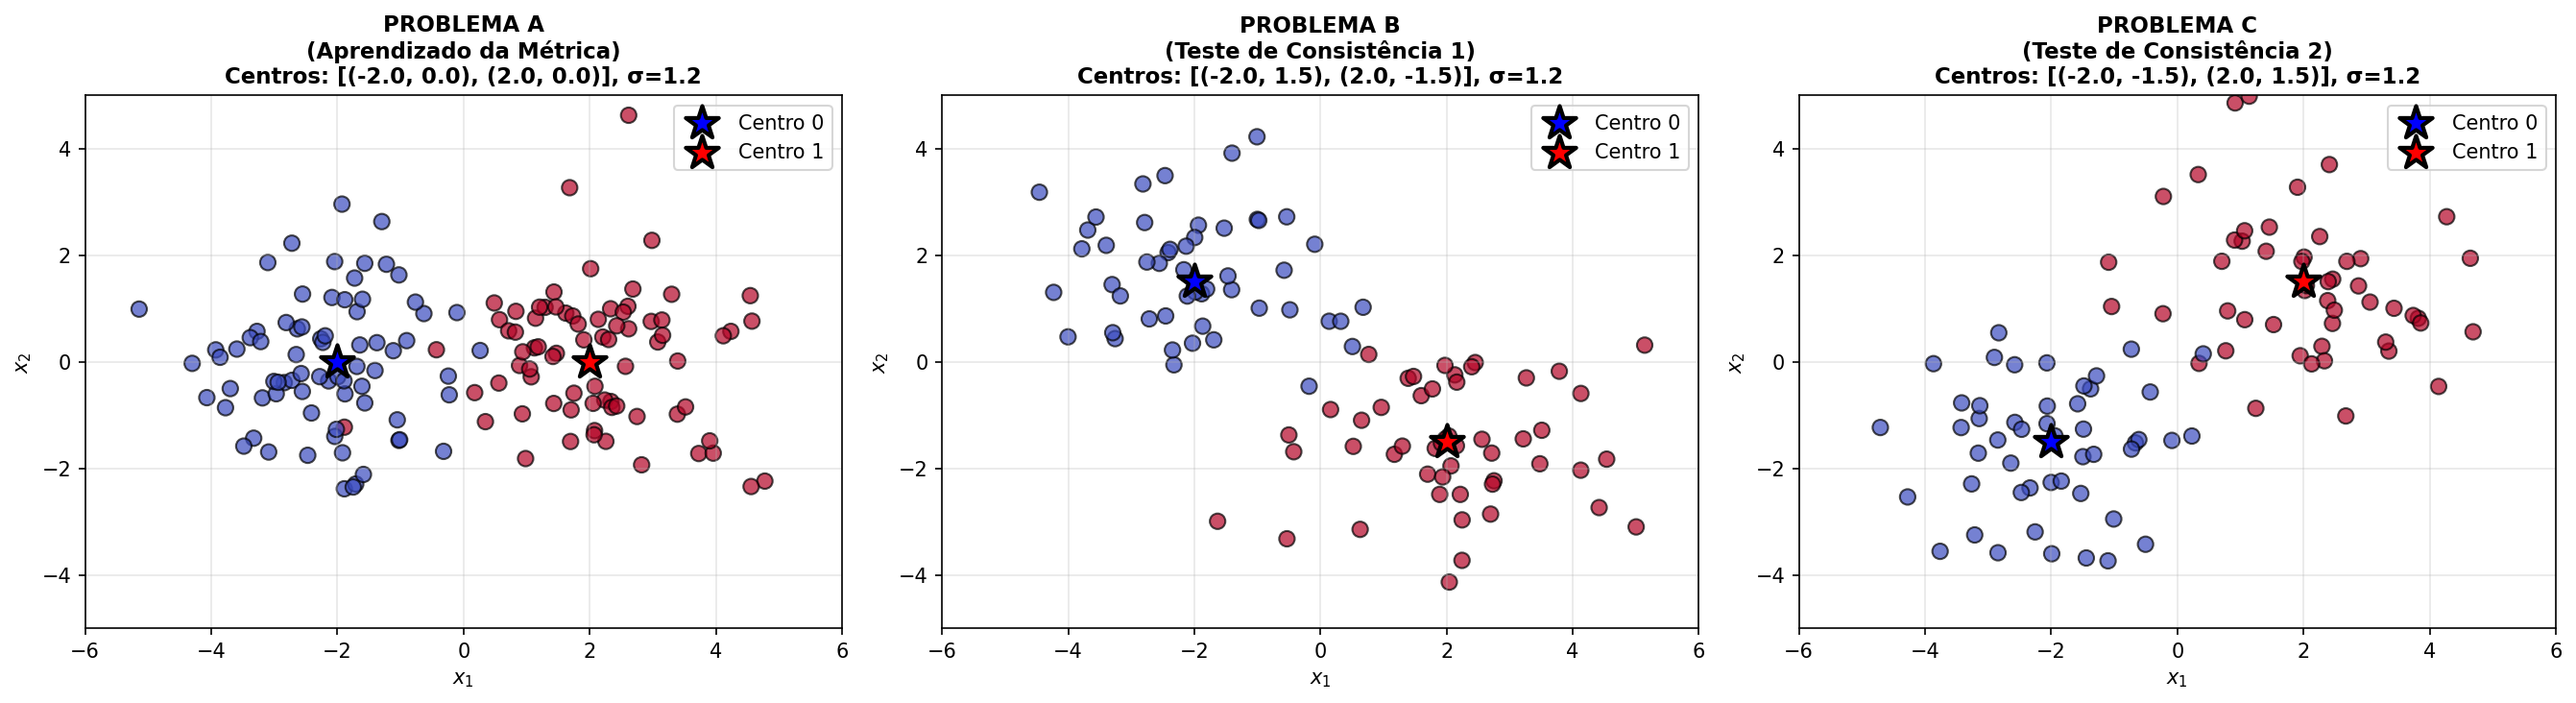
\includegraphics[width=\linewidth,height=0.45\textheight,keepaspectratio]{bloco1_01_problemas_lineares.png}
    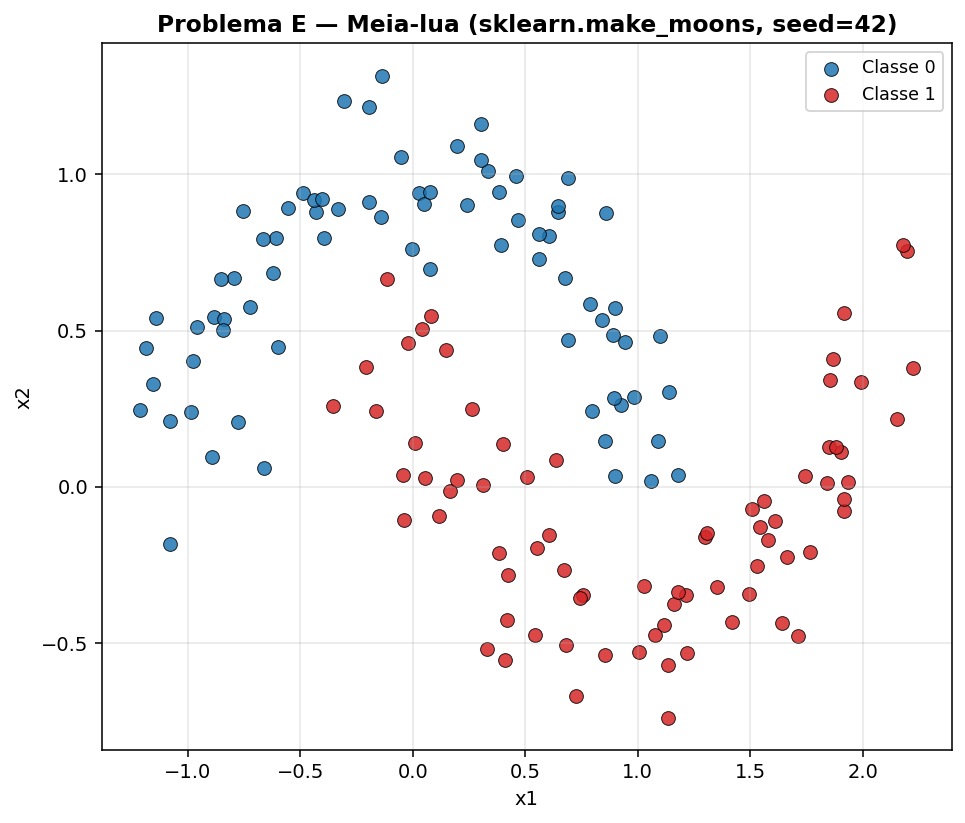
\includegraphics[width=\linewidth,height=0.35\textheight,keepaspectratio]{bloco1_02_problema_d_meialua_seed42_overview.png}
  \end{columns}
\end{frame}

% 11 - Problema A
\begin{frame}{Problema A --- treino da m\'etrica (linear)}
  \scriptsize
  \begin{columns}[T]
    \column{0.55\linewidth}
    \textbf{Prop\'osito:} bancada de treinamento.
    \medskip

    \textbf{Como foi gerado:}
    \begin{enumerate}\setlength\itemsep{0.1em}
      \item \texttt{make\_blobs}
      \item Centr\'oides $(-2{,}0; 0{,}0)$ e $(2{,}0; 0{,}0)$
      \item \texttt{cluster\_std}=1{,}2
      \item $n=150$
    \end{enumerate}
    \textbf{Por qu\^e:} linearmente separ\'avel em $x_1$; fronteira ideal em $x_1=0$.
    \column{0.45\linewidth}
    \tiny
    \texttt{def create\_problem\_a(n=150, seed=42):}\\
    \texttt{\ \ X,y = make\_blobs(}\\
    \texttt{\ \ \ \ centers=[(-2.0,0.0),(2.0,0.0)],}\\
    \texttt{\ \ \ \ cluster\_std=1.2,}\\
    \texttt{\ \ \ \ random\_state=seed)}\\
    \medskip
    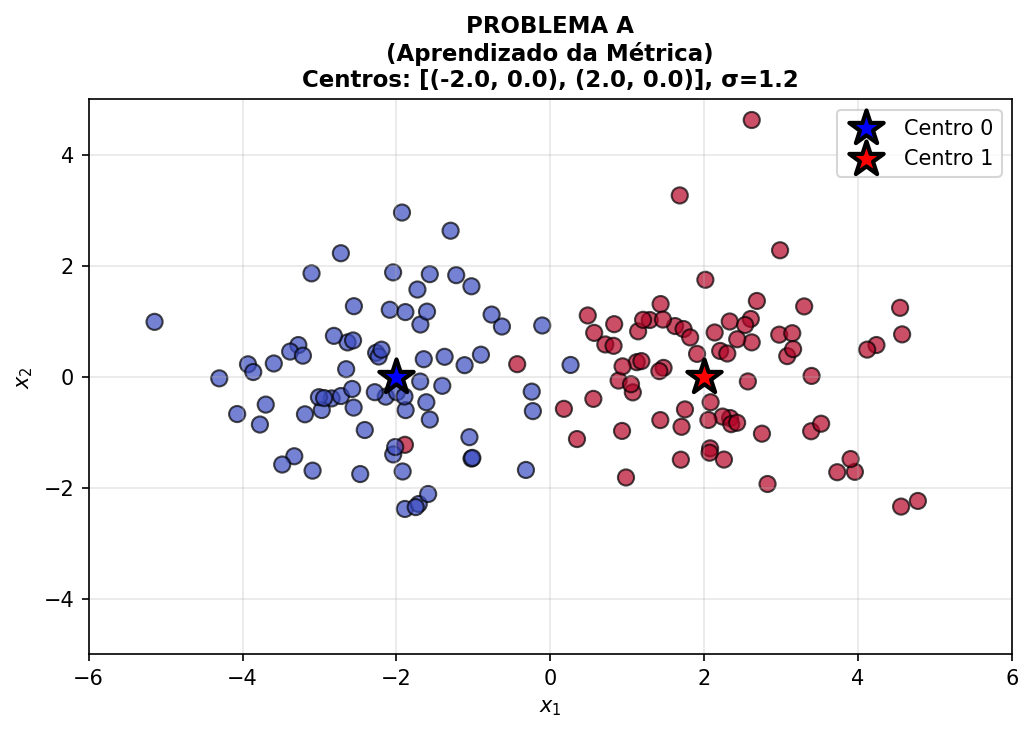
\includegraphics[width=\linewidth,height=0.45\textheight,keepaspectratio]{bloco1_01_problemas_lineares_problema_a.png}
  \end{columns}
\end{frame}

% 12 - Problema B
\begin{frame}{Problema B --- rota\c{c}\~ao HOR\'ARIA agressiva ($\pm 1.5$)}
  \scriptsize
  \begin{columns}[T]
    \column{0.55\linewidth}
    \textbf{Prop\'osito:} testar transfer\^encia de $W$ em geometria deslocada \emph{agressivamente}.
    \medskip

    \textbf{Como foi gerado:}
    \begin{enumerate}\setlength\itemsep{0.1em}
      \item \texttt{make\_blobs}
      \item Centr\'oides $(-2{,}0; +1{,}5)$ e $(2{,}0; -1{,}5)$
      \item \texttt{cluster\_std}=1{,}2
      \item $n=100$
    \end{enumerate}
    \textbf{Por qu\^e:} pareada simetricamente com C ($\pm 1.5$); decis\~ao 14/05/2026 para condi\c{c}\~oes severas.
    \column{0.45\linewidth}
    \tiny
    \texttt{def create\_problem\_b(n=100, seed=43):}\\
    \texttt{\ \ X,y = make\_blobs(}\\
    \texttt{\ \ \ \ centers=[(-2.0,1.5),(2.0,-1.5)],}\\
    \texttt{\ \ \ \ cluster\_std=1.2,}\\
    \texttt{\ \ \ \ random\_state=seed)}\\
    \medskip
    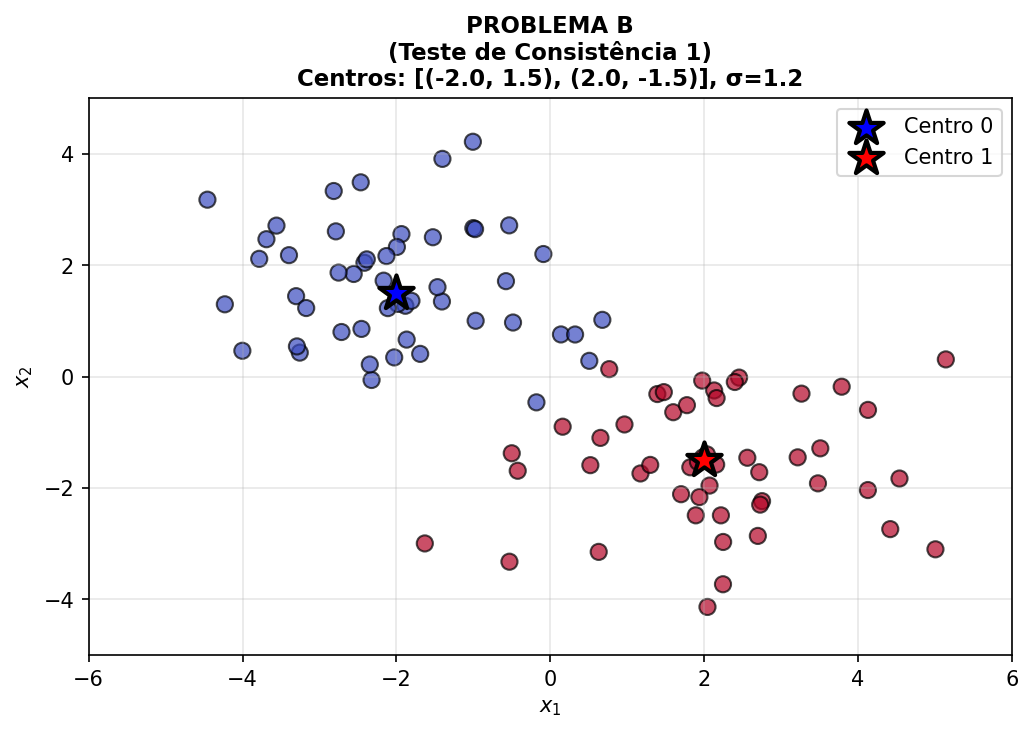
\includegraphics[width=\linewidth,height=0.45\textheight,keepaspectratio]{bloco1_01_problemas_lineares_problema_b.png}
  \end{columns}
\end{frame}

% 13 - Problema C
\begin{frame}{Problema C --- rota\c{c}\~ao ANTI-HOR\'ARIA agressiva ($\pm 1.5$)}
  \scriptsize
  \begin{columns}[T]
    \column{0.55\linewidth}
    \textbf{Prop\'osito:} mesma severidade de B, dire\c{c}\~ao OPOSTA. Controle contra vi\'es sistem\'atico.
    \medskip

    \textbf{Como foi gerado:}
    \begin{enumerate}\setlength\itemsep{0.1em}
      \item \texttt{make\_blobs}
      \item Centr\'oides $(-2{,}0; -1{,}5)$ e $(2{,}0; +1{,}5)$
      \item \texttt{cluster\_std}=1{,}2
      \item $n=100$
    \end{enumerate}
    \textbf{Por qu\^e:} alterado ap\'os reuni\~ao 30/04/2026 ($\sim$120s) --- C antes era c\'opia de B.
    \column{0.45\linewidth}
    \tiny
    \texttt{def create\_problem\_c(n=100, seed=44):}\\
    \texttt{\ \ X,y = make\_blobs(}\\
    \texttt{\ \ \ \ centers=[(-2.0,-1.5),(2.0,1.5)],}\\
    \texttt{\ \ \ \ cluster\_std=1.2,}\\
    \texttt{\ \ \ \ random\_state=seed)}\\
    \medskip
    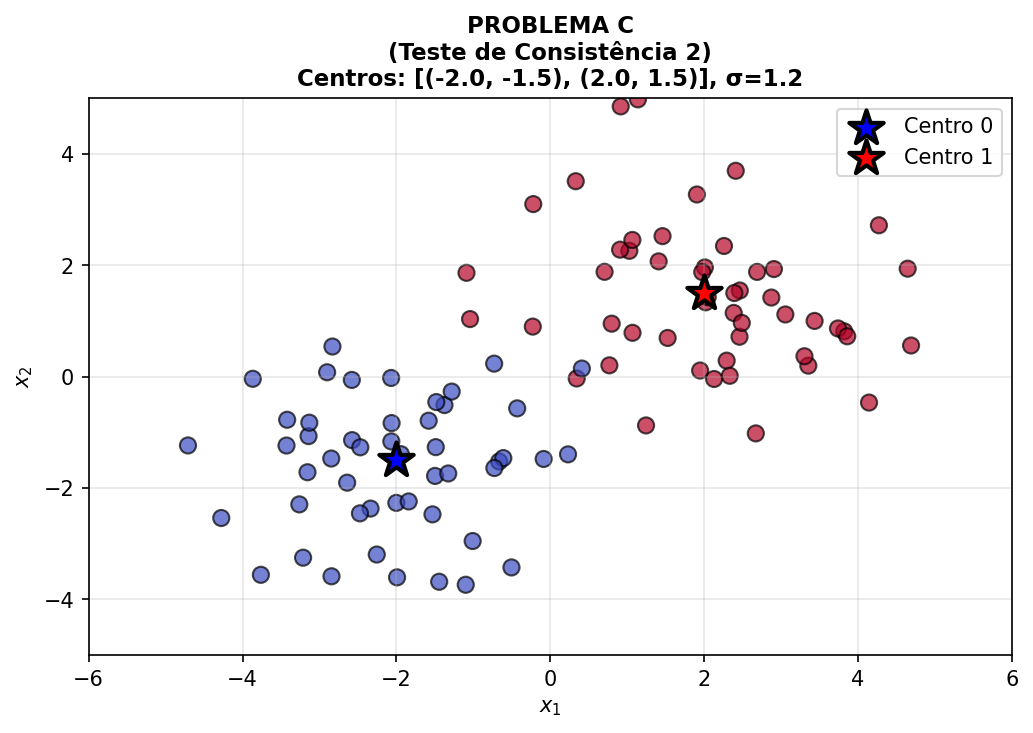
\includegraphics[width=\linewidth,height=0.45\textheight,keepaspectratio]{bloco1_01_problemas_lineares_problema_c.png}
  \end{columns}
\end{frame}

% 14 - Problema D meia-lua
\begin{frame}{Problema D --- meia-lua (n\~ao-linear sint\'etico)}
  \scriptsize
  \begin{columns}[T]
    \column{0.55\linewidth}
    \textbf{Prop\'osito:} caso can\^onico de fronteira n\~ao-linear (reuni\~ao 30/04 $\sim$2853s).
    \medskip

    \textbf{Como foi gerado:}
    \begin{enumerate}\setlength\itemsep{0.1em}
      \item \texttt{sklearn.datasets.make\_moons}
      \item $n = 150$
      \item \texttt{noise}=0{,}15
    \end{enumerate}
    Problema-controle POSITIVO para R3/R4 --- esperamos ganho de n\~ao-linearidade aqui.
    \column{0.45\linewidth}
    \tiny
    \texttt{from sklearn.datasets import make\_moons}\\
    \texttt{def create\_problem\_d\_meialua(}\\
    \texttt{\ \ \ \ n=150, seed=46):}\\
    \texttt{\ \ X,y = make\_moons(}\\
    \texttt{\ \ \ \ n\_samples=n, noise=0.15,}\\
    \texttt{\ \ \ \ random\_state=seed)}\\
    \medskip
    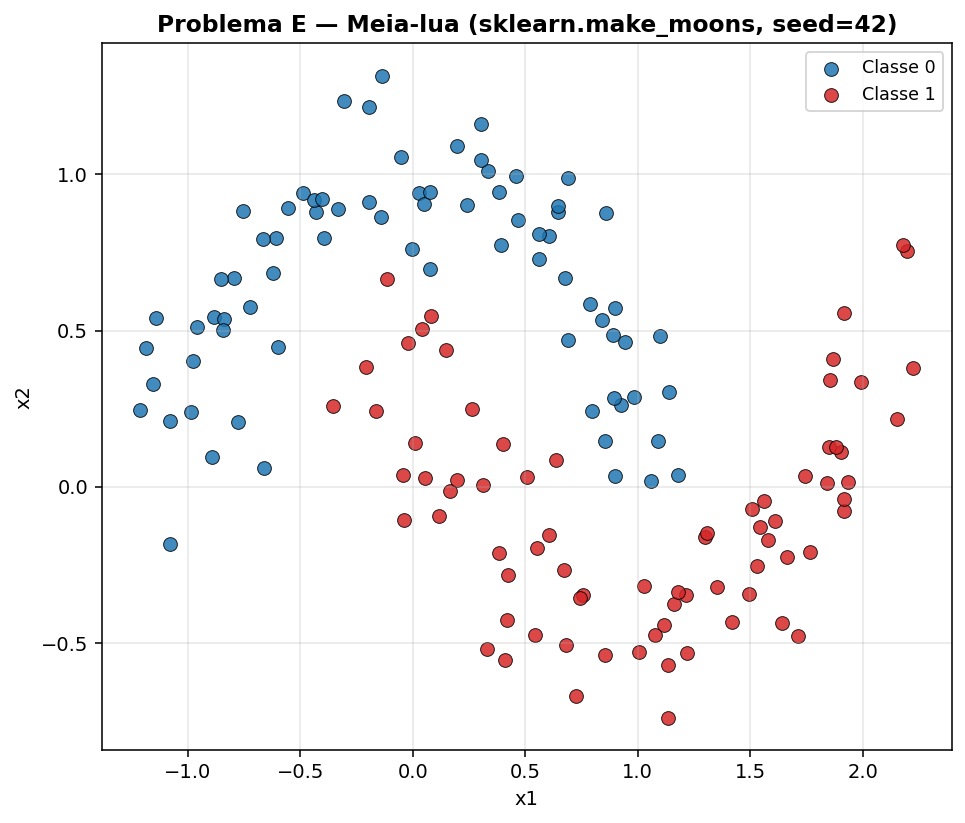
\includegraphics[width=\linewidth,height=0.45\textheight,keepaspectratio]{bloco1_02_problema_d_meialua_seed42_overview.png}
  \end{columns}
\end{frame}

% 15 - Oracle
\begin{frame}{Oracle Validation --- sanity check}
  \scriptsize
  \begin{columns}[T]
    \column{0.45\linewidth}
    Antes de aplicar Perceptron/NNLS ao LLM, validar com $W$ conhecido:
    \begin{enumerate}
      \item Gerar dados sint\'eticos.
      \item Rotular com $W_{\text{oracle}}$ (ex.\ $[0{,}1;\ 2{,}0]$).
      \item Aprender $\hat W$.
      \item Comparar $\hat W$ vs $W_{\text{oracle}}$ (cosseno).
    \end{enumerate}
    \textbf{3 configs:} x2\_dom, x1\_dom, forte\_aniso. Sem este check, qualquer achado sobre o LLM ficaria comprometido.
    \column{0.55\linewidth}
    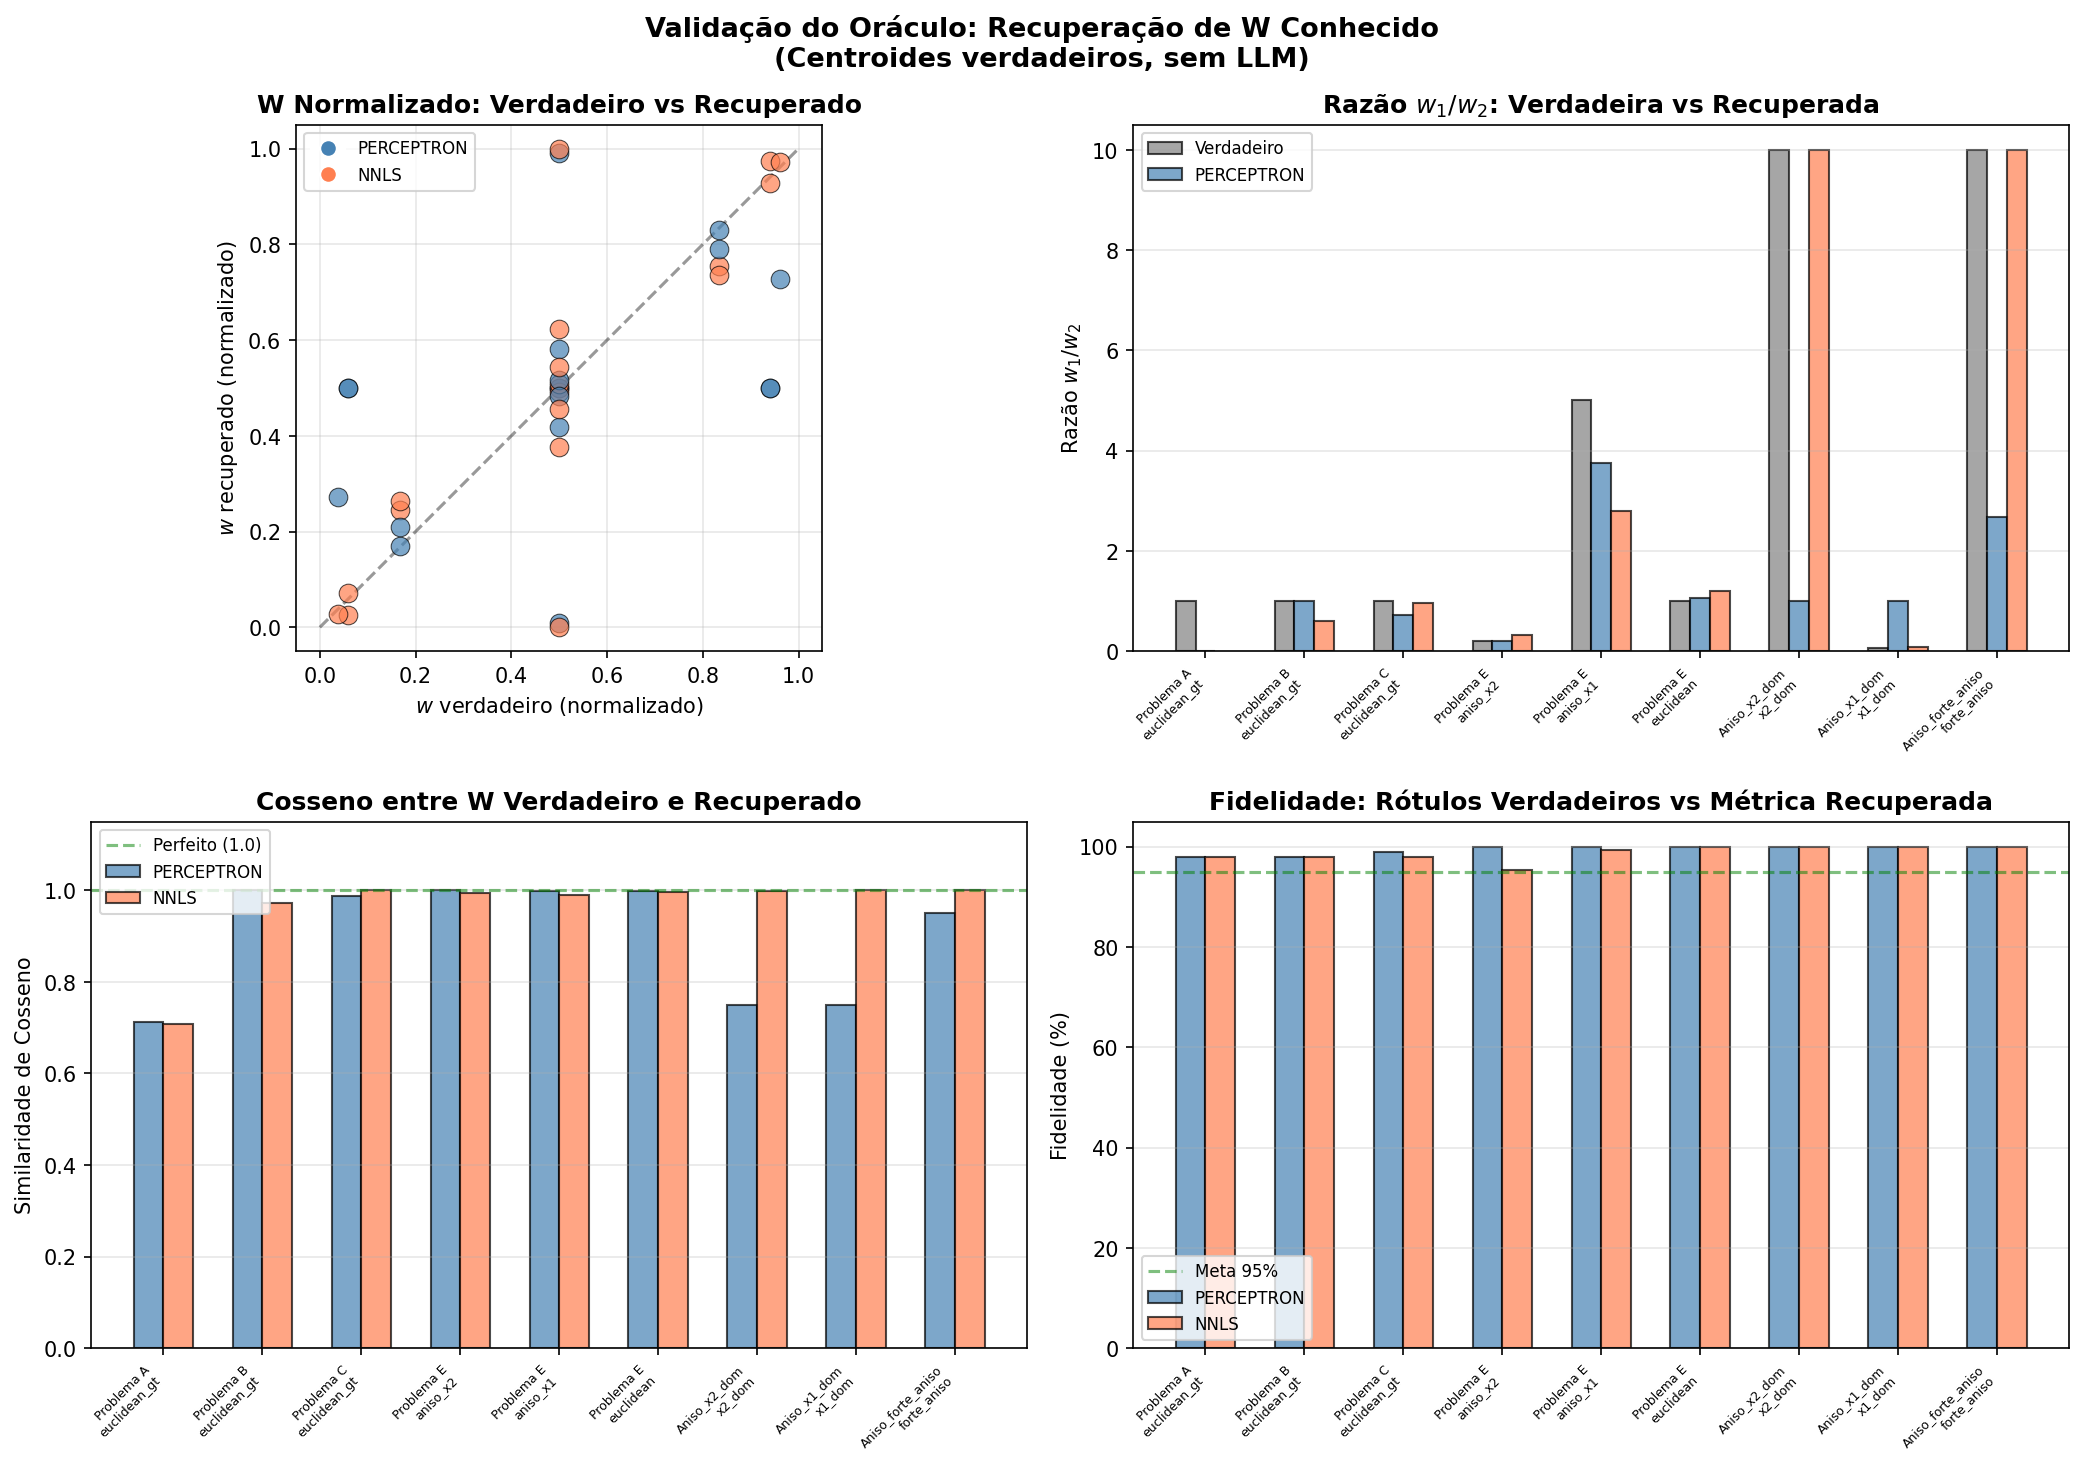
\includegraphics[width=\linewidth,height=0.7\textheight,keepaspectratio]{bloco1_03_oracle_w_recovery.png}
  \end{columns}
\end{frame}

% 16 - Fase A descricao
\begin{frame}{Fase A --- aprendizado da m\'etrica}
  \footnotesize
  \begin{enumerate}
    \item LLM recebe 150 pontos do Problema A em \textbf{zero-shot}.
    \item Responde A ou B com $T=0$.
    \item 150 respostas formam $(X, y_{\text{LLM}})$.
    \item \textbf{Centr\'oides recalculados a partir de $y_{\text{LLM}}$} --- ancoramos no que o LLM ACHA serem as classes.
    \item Perceptron Estruturado e NNLS aprendem $W$ independentemente.
    \item Fidelidade = \% decis\~oes do LLM reproduzidas pela m\'etrica.
  \end{enumerate}
\end{frame}

% 17 - Fase A W e fidelidade
\begin{frame}{Fase A --- $W$ aprendido e fidelidade (seed 42)}
  \scriptsize
  \begin{columns}[T]
    \column{0.4\linewidth}
    \textbf{Achados desta execu\c{c}\~ao:}
    \begin{tabular}{lc}
      \toprule
      Algoritmo & Fidelidade \\
      \midrule
      Perceptron & 82{,}0\% \\
      NNLS       & 82{,}7\% \\
      \bottomrule
    \end{tabular}
    \medskip

    Cosseno $W_{\text{perc}} \cdot W_{\text{nnls}}$: alta concord\^ancia (visualizado no slide 19).
    \column{0.6\linewidth}
    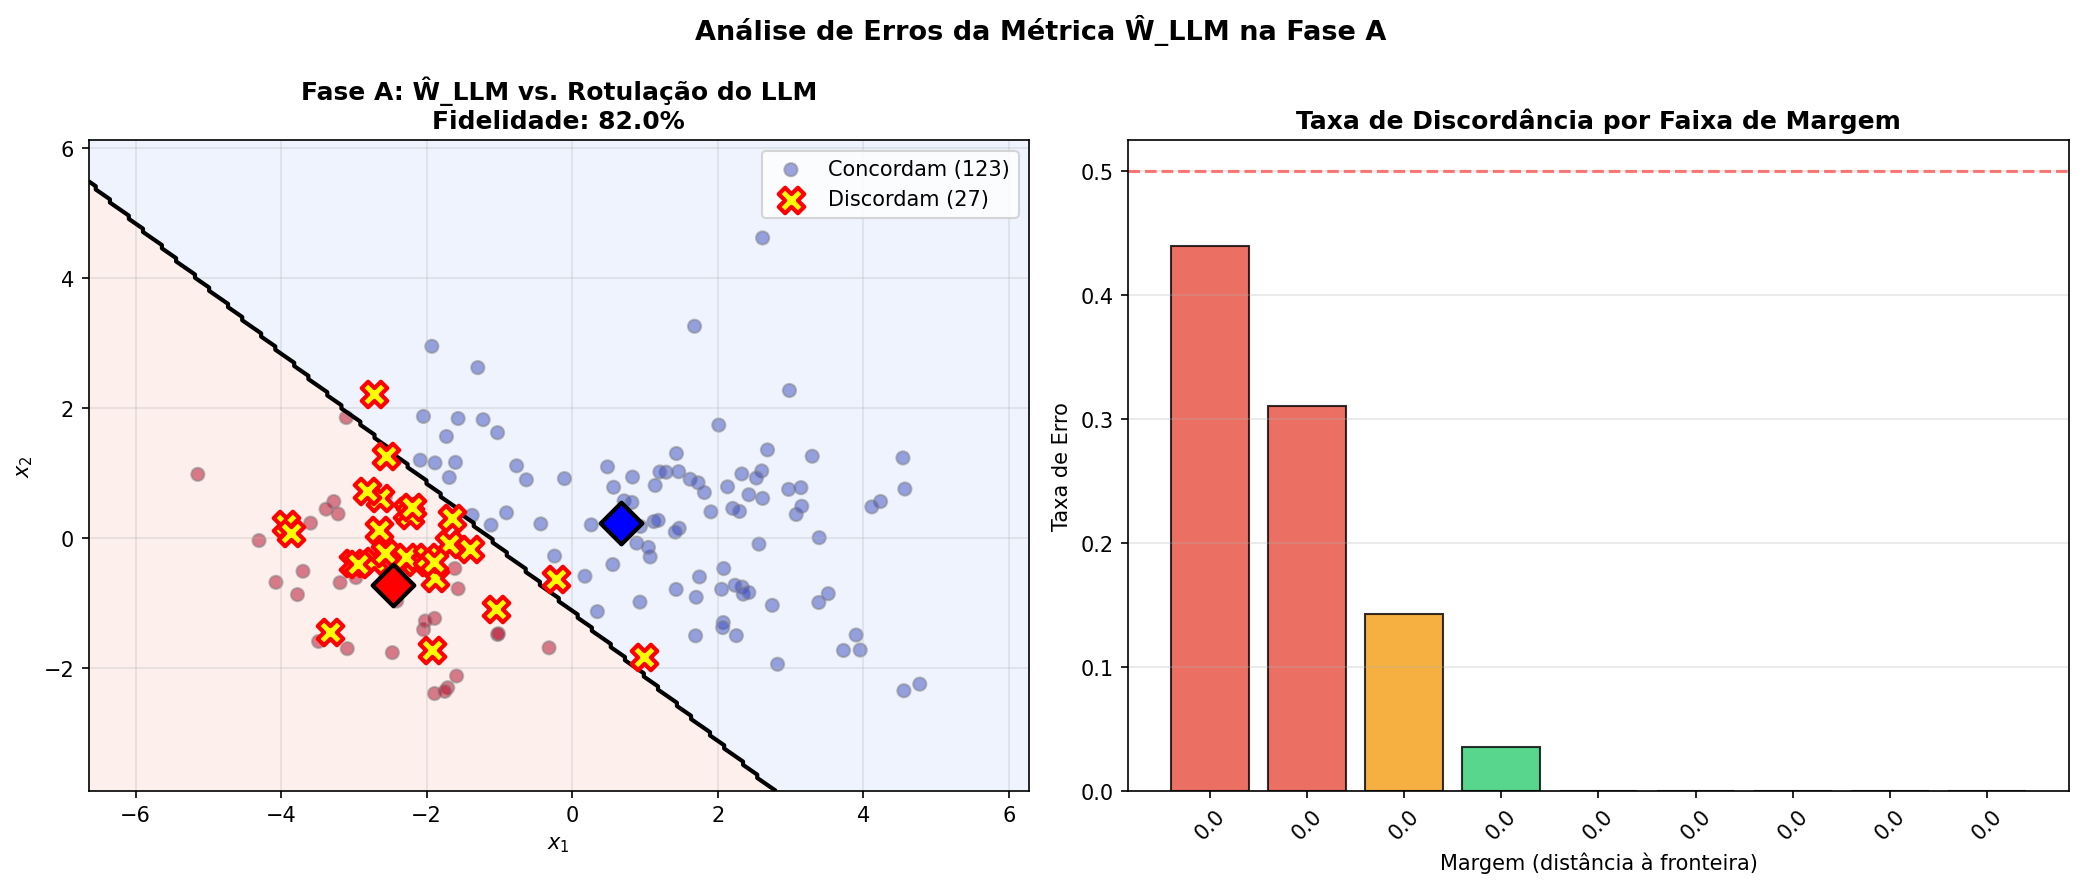
\includegraphics[width=\linewidth,height=0.7\textheight,keepaspectratio]{bloco1_05_fase_a_errors_seed42.png}
  \end{columns}
\end{frame}

% 18 - distribuicao W
\begin{frame}{Fase A --- distribui\c{c}\~ao de $W$ (smoke, seed 42)}
  \scriptsize
  \begin{center}
    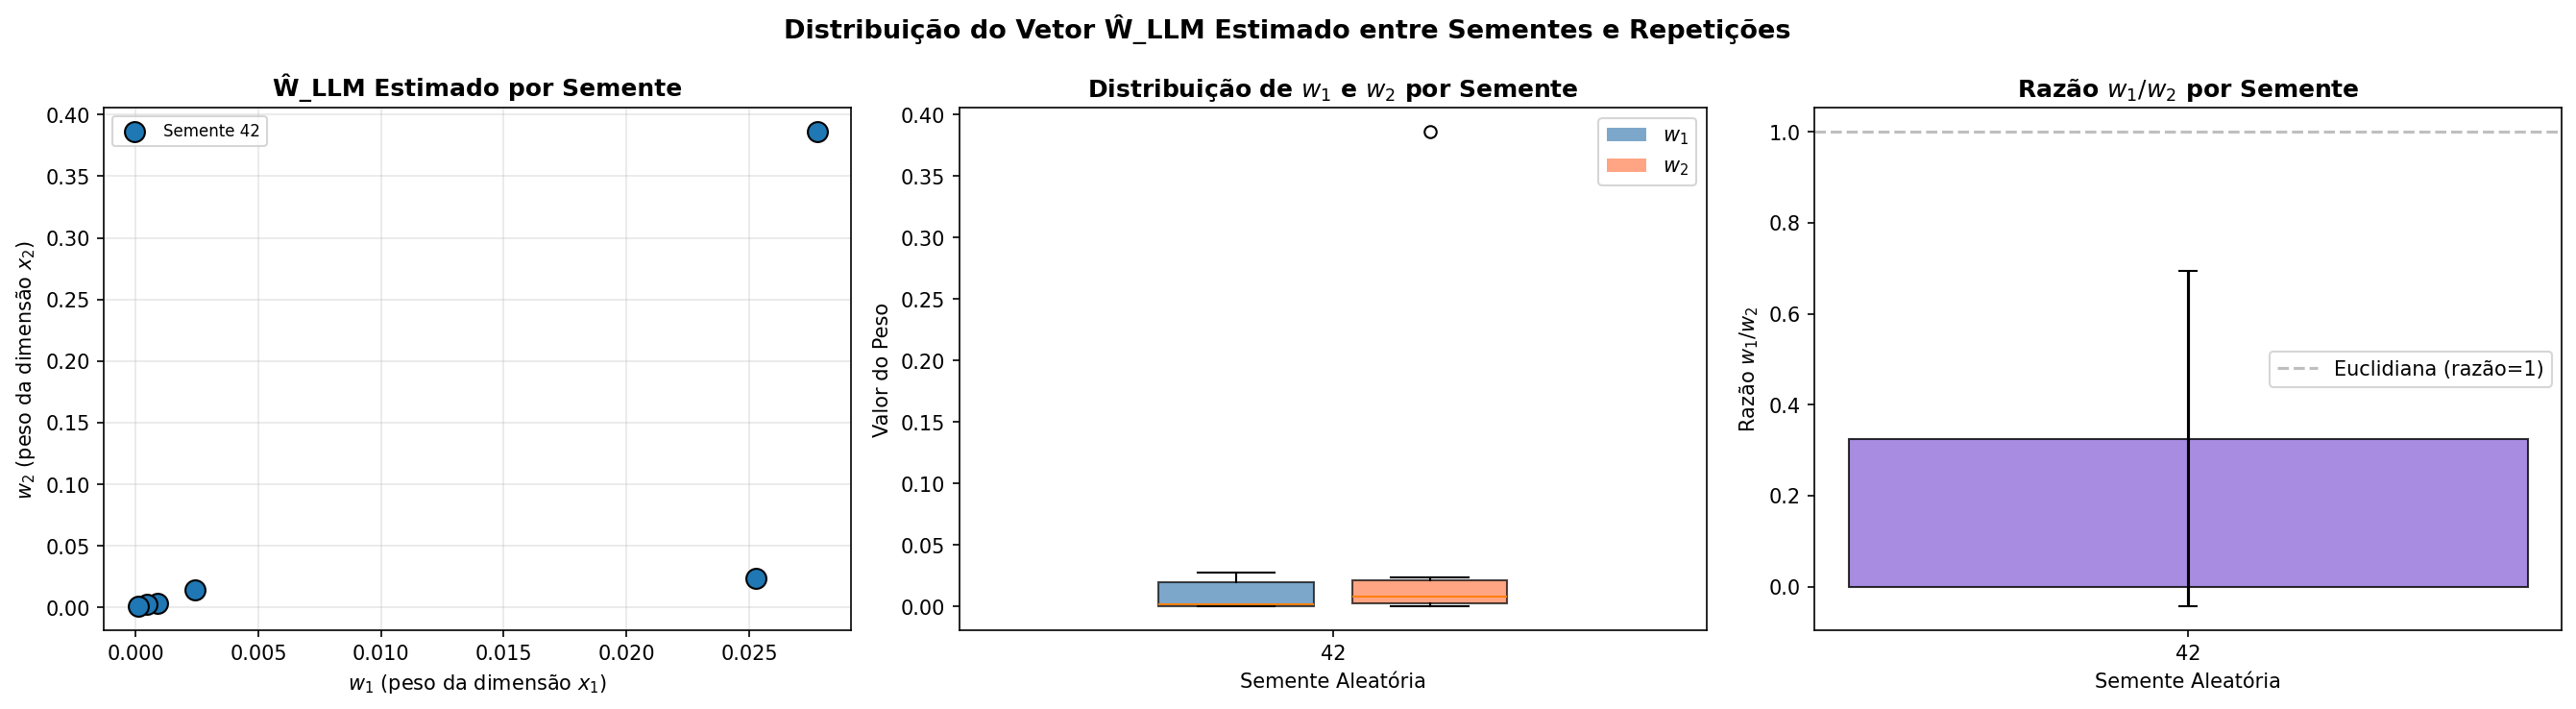
\includegraphics[width=0.85\linewidth,height=0.7\textheight,keepaspectratio]{bloco1_06_w_distribution.png}
  \end{center}
  $W$ estimado pelo Perceptron e pelo NNLS (raz\~ao, boxplot, scatter). Em produ\c{c}\~ao (3 seeds $\times$ 3 reps), comparar estabilidade entre execu\c{c}\~oes.
\end{frame}

% 19 - Algorithm comparison
\begin{frame}{Fase A --- Perceptron $\times$ NNLS}
  \scriptsize
  \begin{center}
    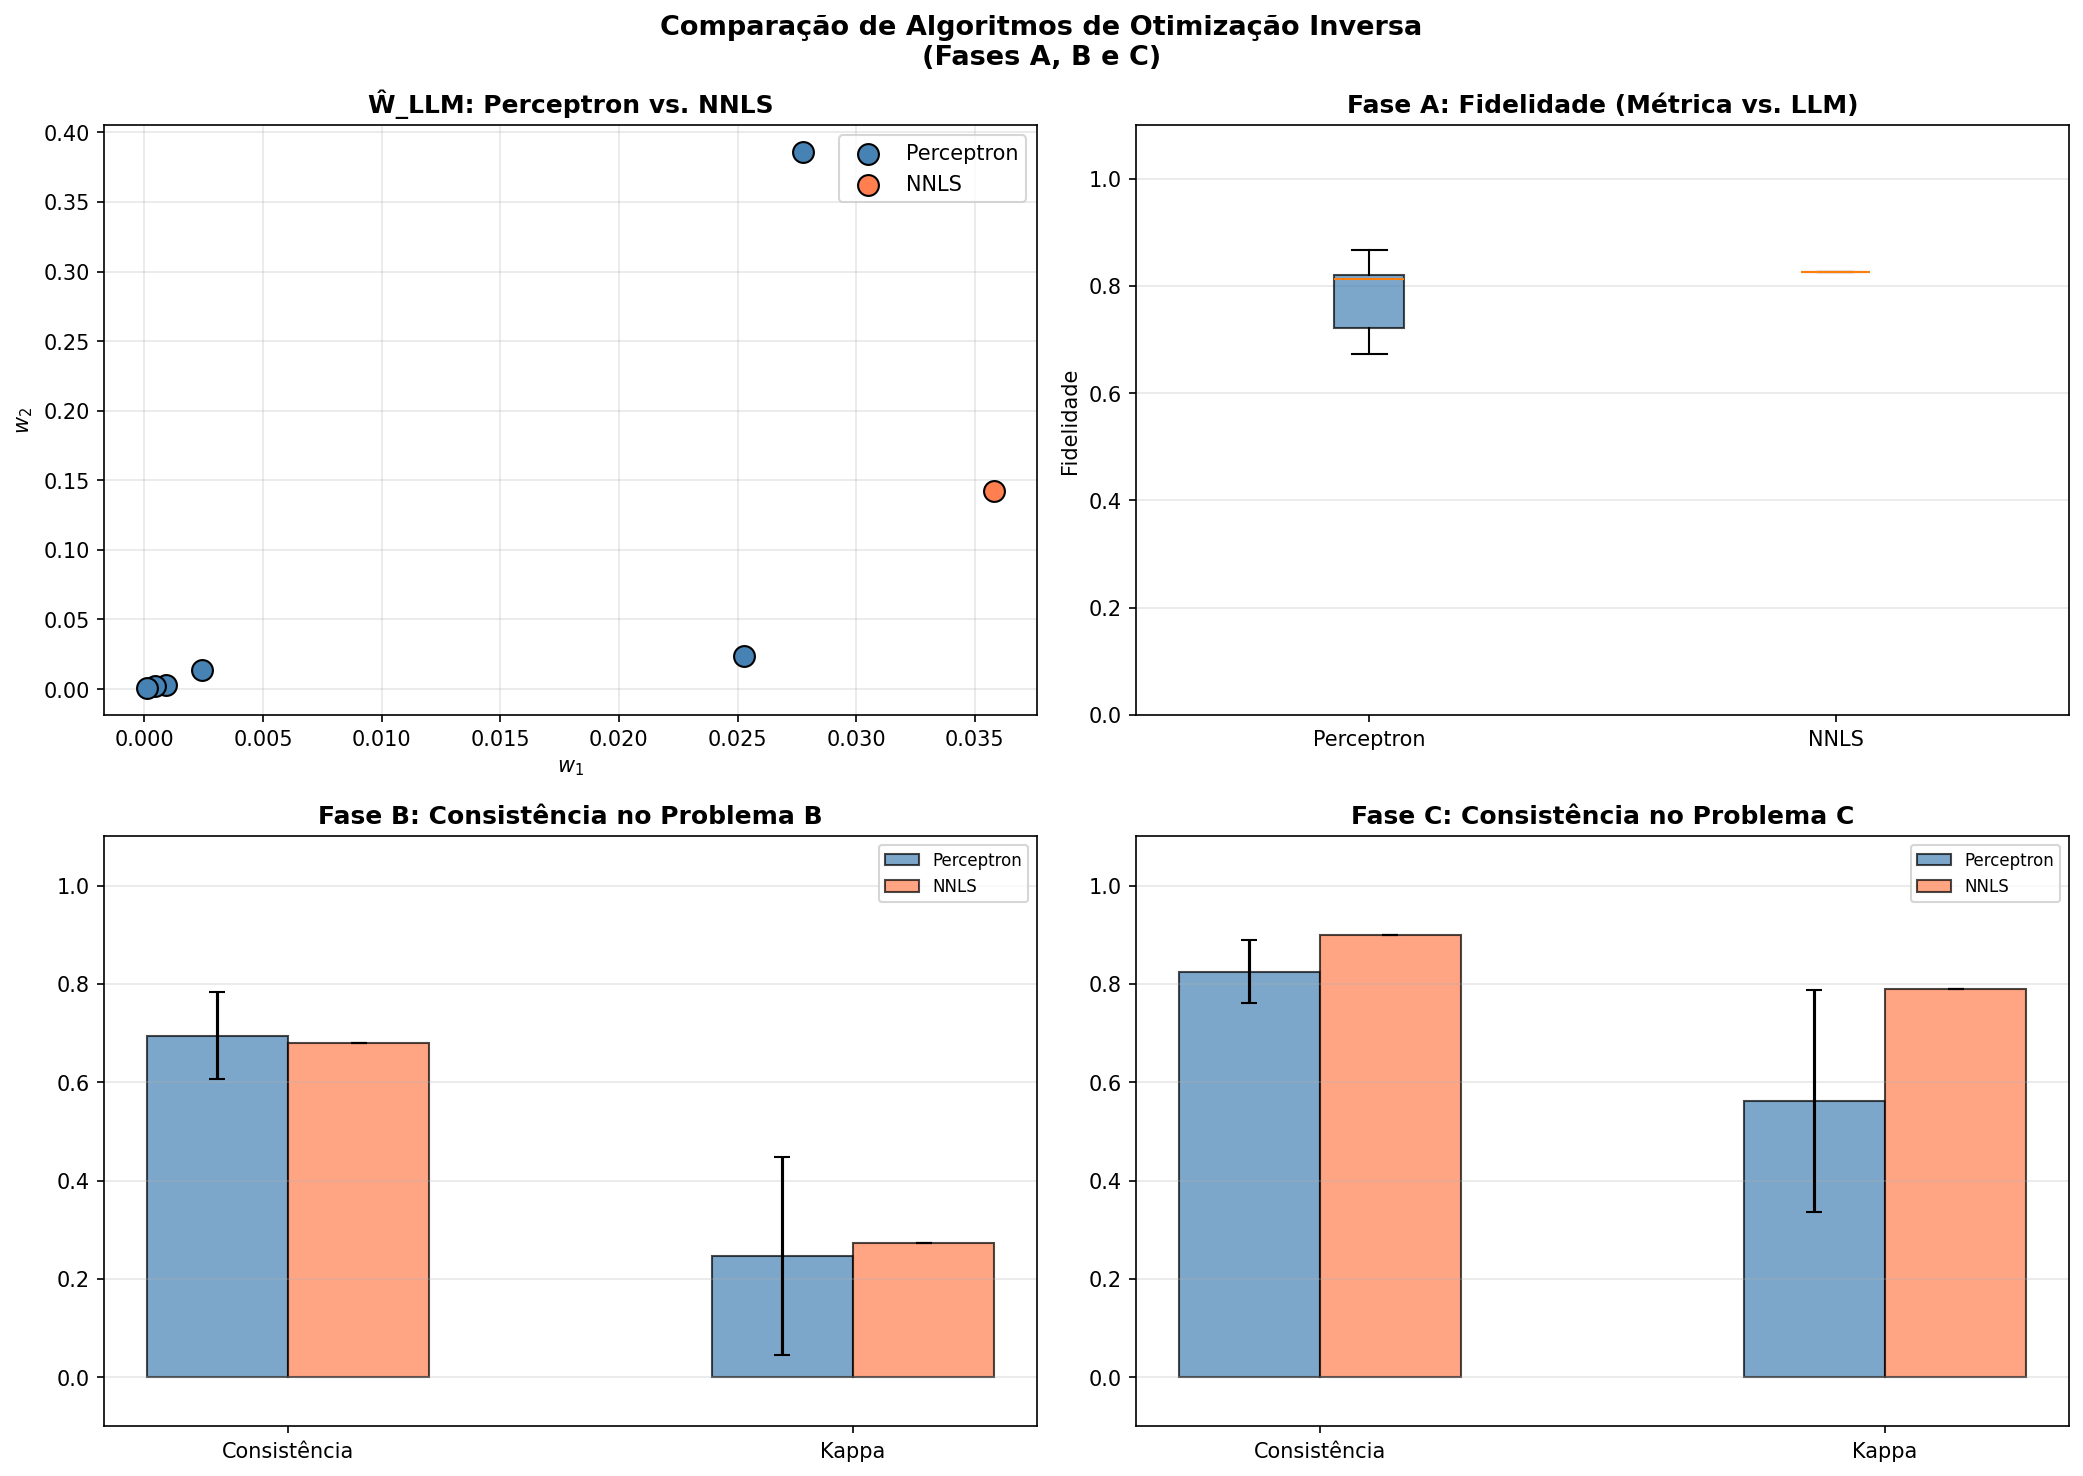
\includegraphics[width=0.9\linewidth,height=0.75\textheight,keepaspectratio]{bloco1_07_algorithm_comparison.png}
  \end{center}
  Robustez ao m\'etodo de estima\c{c}\~ao: ambos os algoritmos chegam ao mesmo $W$.
\end{frame}

% 20 - Fidelidade vs Acuracia
\begin{frame}{Fidelidade vs Acur\'acia (distin\c{c}\~ao cr\'itica)}
  \footnotesize
  \begin{itemize}
    \item \textbf{FIDELIDADE} = \% decis\~oes do LLM reproduzidas pela m\'etrica = quanto a m\'etrica \emph{modela o LLM}.
    \item \textbf{ACUR\'ACIA LLM vs real} = \% decis\~oes do LLM coincidem com ground truth = quanto o LLM \emph{est\'a correto}.
  \end{itemize}
  \medskip
  \textbf{Achado nesta execu\c{c}\~ao} (seed 42, Problema A, zero-shot):
  \begin{itemize}
    \item Fidelidade Perceptron: 82{,}0\%
    \item Fidelidade NNLS: 82{,}7\%
  \end{itemize}
  \textbf{Implica\c{c}\~ao:} medimos CONSIST\^ENCIA INTERNA (H1), n\~ao CORRE\c{C}\~AO. H1 \'e ortogonal a "o crit\'erio est\'a correto".
\end{frame}

% 21 - Fases B/C centroides
\begin{frame}{Fases B/C --- centr\'oides LOCAIS vs TRANSFERIDOS}
  \footnotesize
  Em B/C podemos usar:
  \begin{itemize}
    \item \textbf{LOCAIS} --- recalculados em B/C a partir de $y_{\text{LLM}}$ na pr\'opria fase.
    \item \textbf{TRANSFERIDOS} --- reutilizados do Problema A.
  \end{itemize}
  \medskip
  \textbf{Padr\~ao adotado:} LOCAIS --- mais fi\'eis \`a decis\~ao real do LLM em cada problema. Transferidos ficam como ablativo opcional.
\end{frame}

% 22 - Fases B/C resultados
\begin{frame}{Fases B e C --- resultados (seed 42, rota\c{c}\~ao $\pm 1.5$)}
  \scriptsize
  \begin{center}
  \begin{tabular}{lcc}
    \toprule
    Fase / Algoritmo & Consist\^encia & Kappa \\
    \midrule
    \textbf{Fase B} (rot.\ hor\'aria) Perceptron & 70{,}0\% & 0{,}330 \\
    \textbf{Fase B} NNLS                         & 68{,}0\% & 0{,}286 \\
    \textbf{Fase C} (rot.\ anti-hor\'aria) Perceptron & \textbf{89{,}0\%} & \textbf{0{,}771} \\
    \textbf{Fase C} NNLS                              & \textbf{91{,}0\%} & \textbf{0{,}810} \\
    \bottomrule
  \end{tabular}
  \end{center}
  \medskip
  \begin{center}
    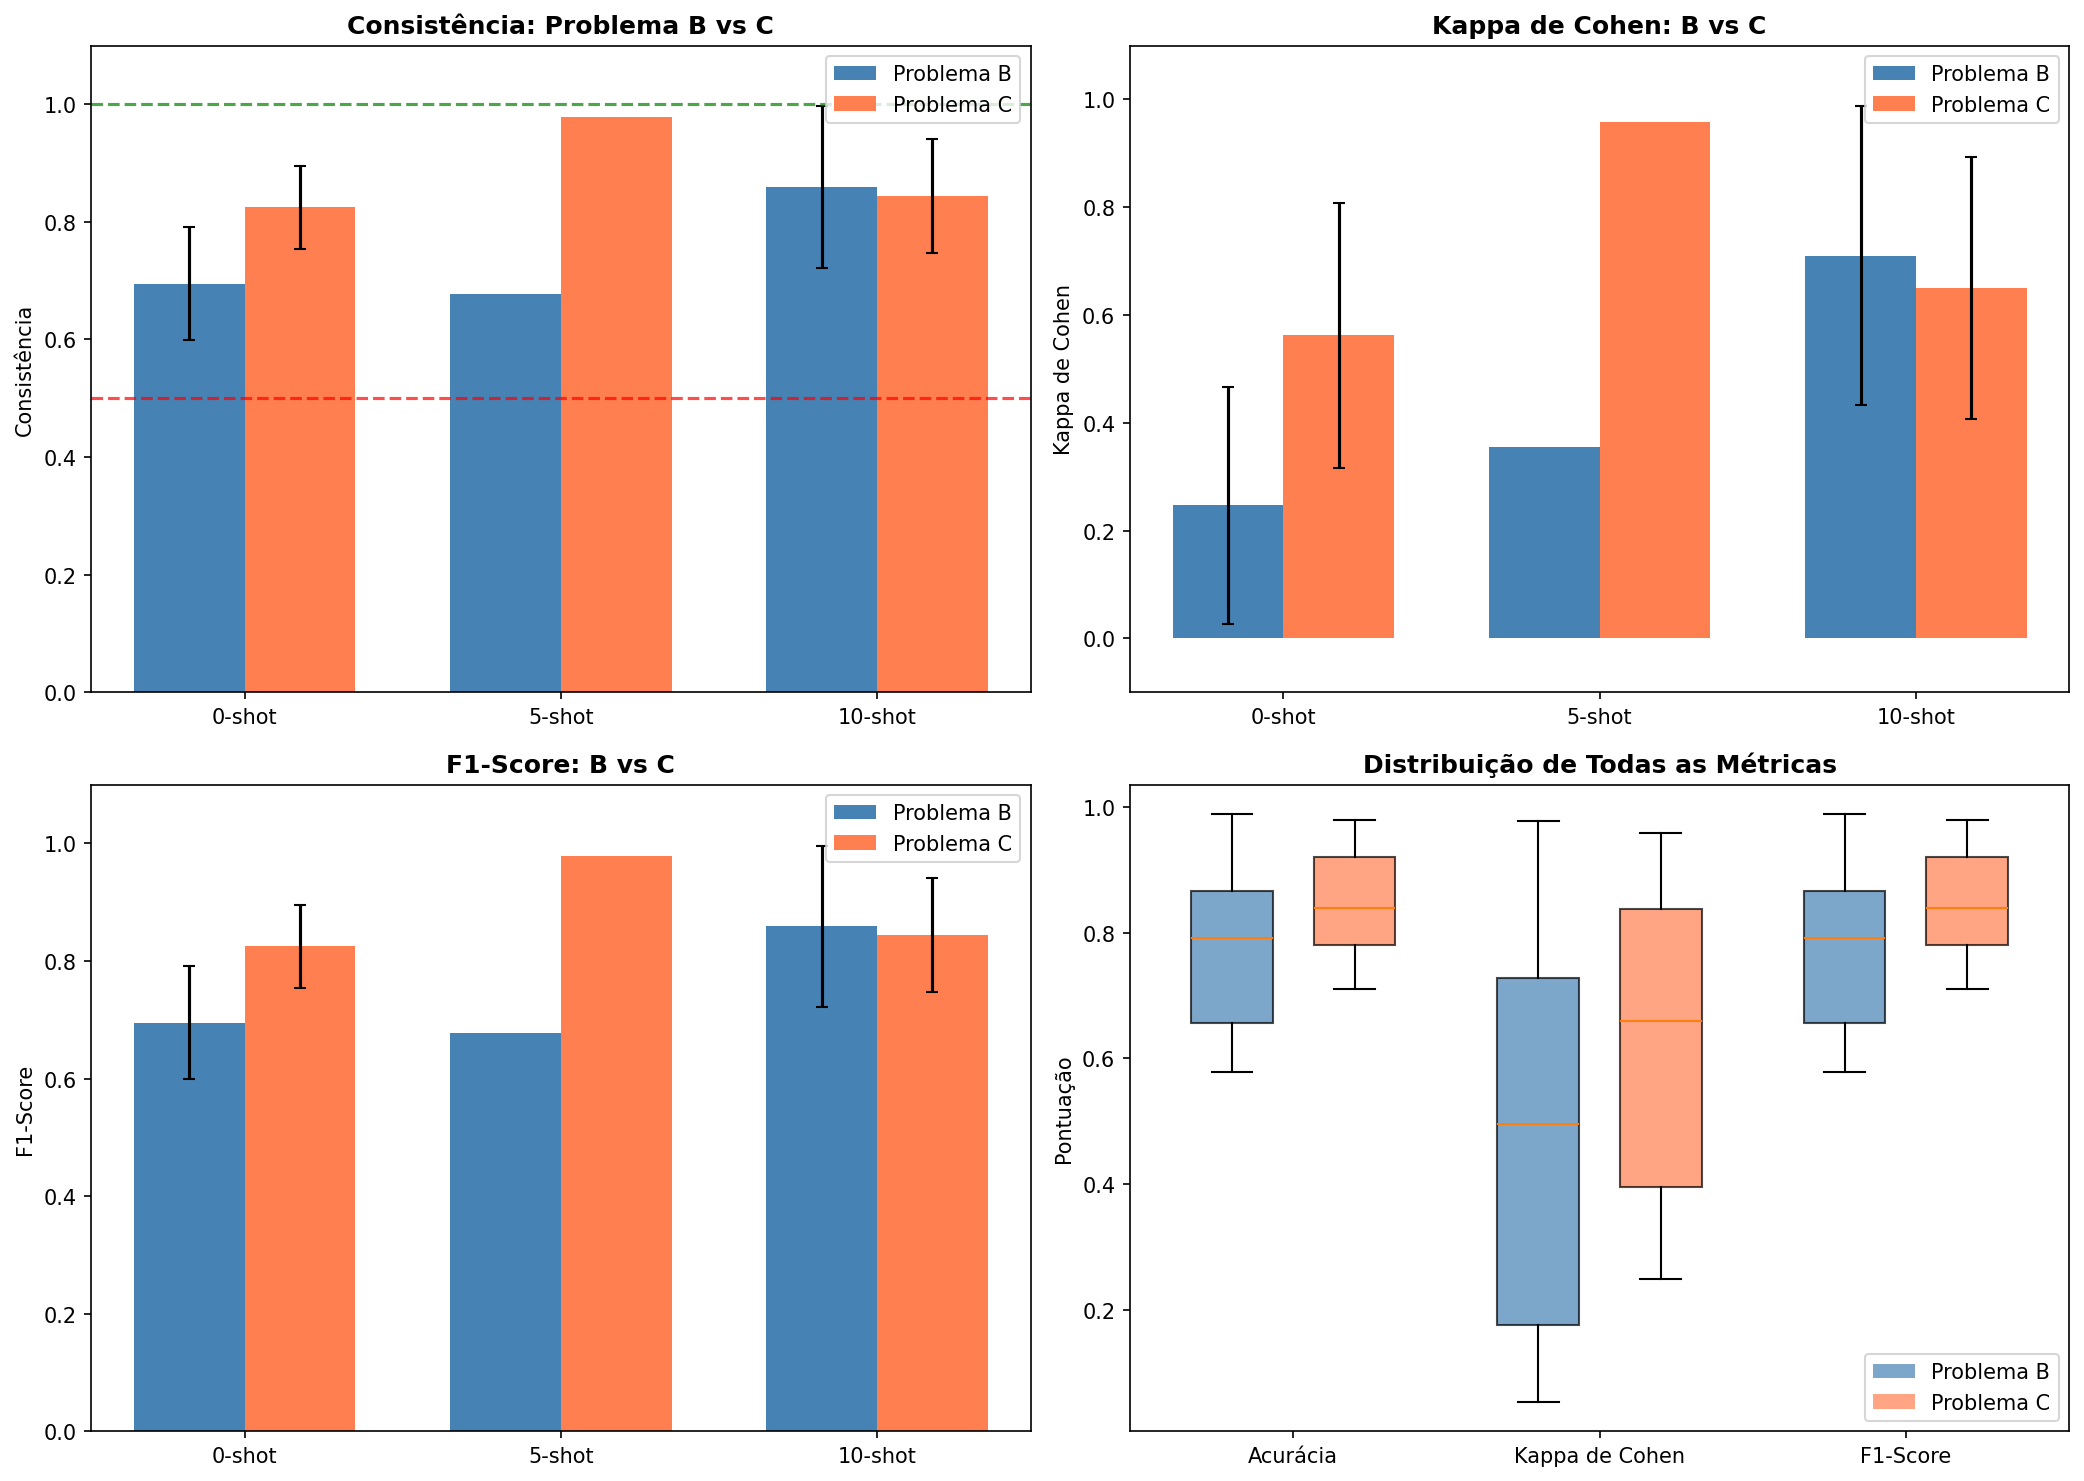
\includegraphics[width=0.7\linewidth,height=0.45\textheight,keepaspectratio]{bloco1_09_consistency_extended.png}
  \end{center}
  \textbf{Observa\c{c}\~ao:} C transfere muito bem; B \'e mais dif\'icil. Em produ\c{c}\~ao 3 seeds estabilizar\'a a tend\^encia.
\end{frame}

% 23 - R3/R4 lineares
\begin{frame}{R2 $\to$ R3 $\to$ R4 nos lineares A/B/C}
  \scriptsize
  \begin{columns}[T]
    \column{0.45\linewidth}
    \textbf{Augmenta\c{c}\~ao de features:}
    \begin{itemize}
      \item R2: $(x_1, x_2)$
      \item R3: $+\, x_1 x_2$ (hip\'erbole)
      \item R4: $+\, x_1^2, x_2^2$ (elipse)
    \end{itemize}
    \medskip
    \textbf{Expectativa:} ganho $\approx 0$ em A/B/C lineares --- linear j\'a \'e suficiente.
    \column{0.55\linewidth}
    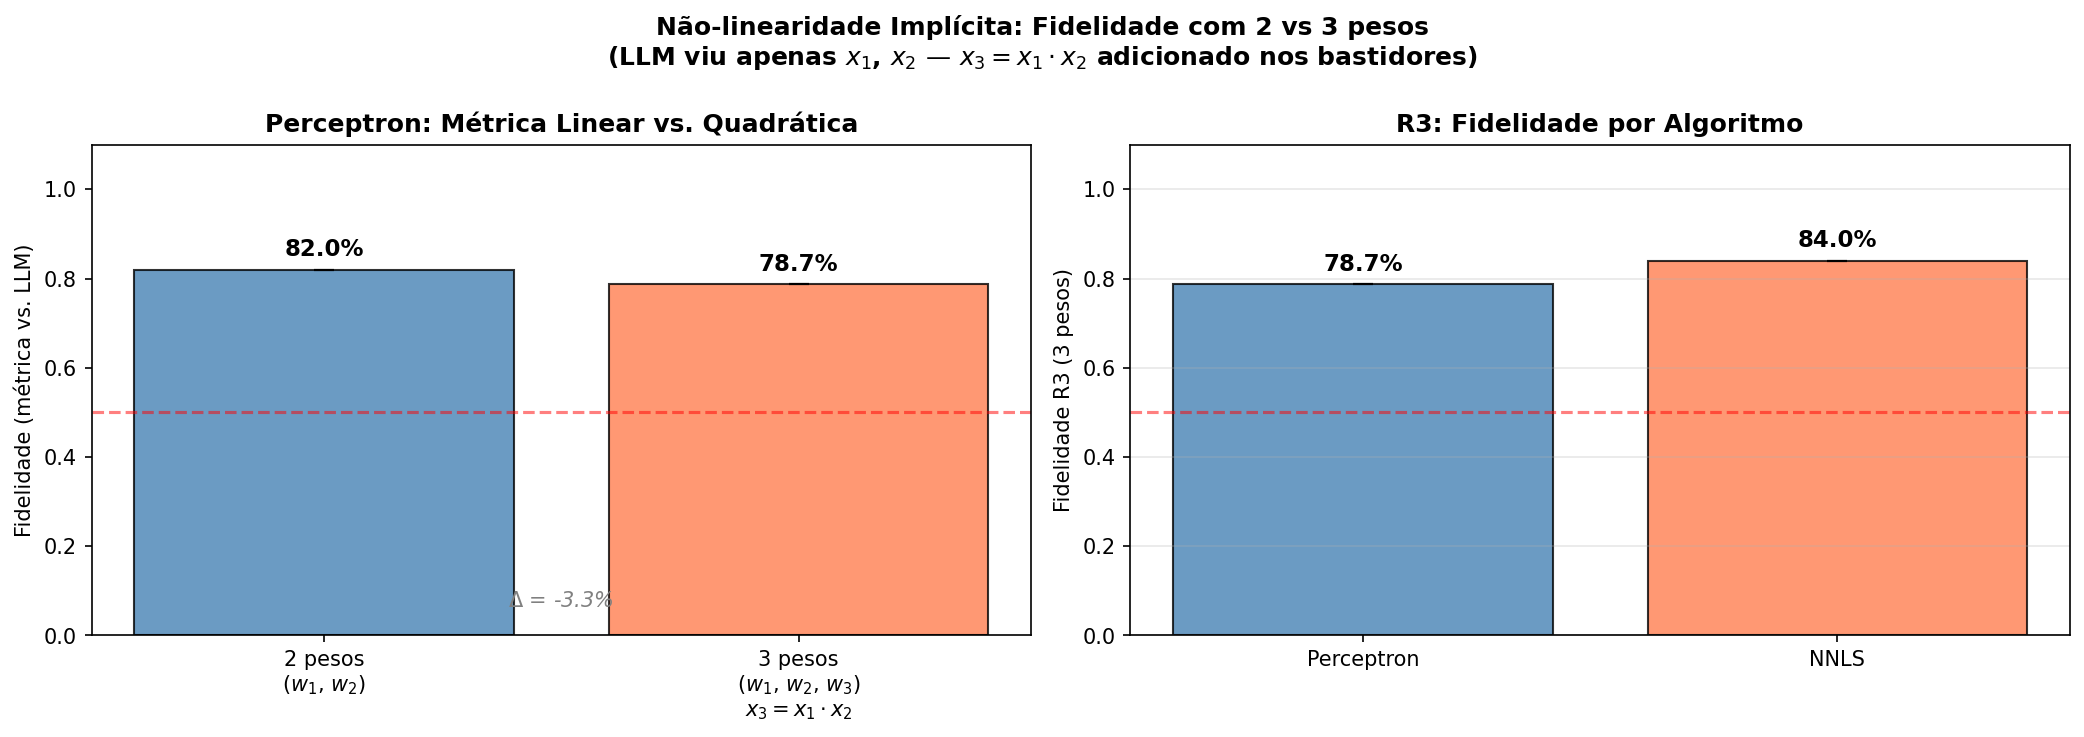
\includegraphics[width=\linewidth,height=0.7\textheight,keepaspectratio]{bloco1_10_r3r4_comparison.png}
  \end{columns}
\end{frame}

% 24 - R3/R4 meia-lua
\begin{frame}{R2 $\to$ R3 $\to$ R4 na meia-lua (Problema D)}
  \scriptsize
  Pipeline externo gera CSV \texttt{bloco23\_external\_phase\_a\_<ts>.csv}.
  \medskip
  \begin{center}
    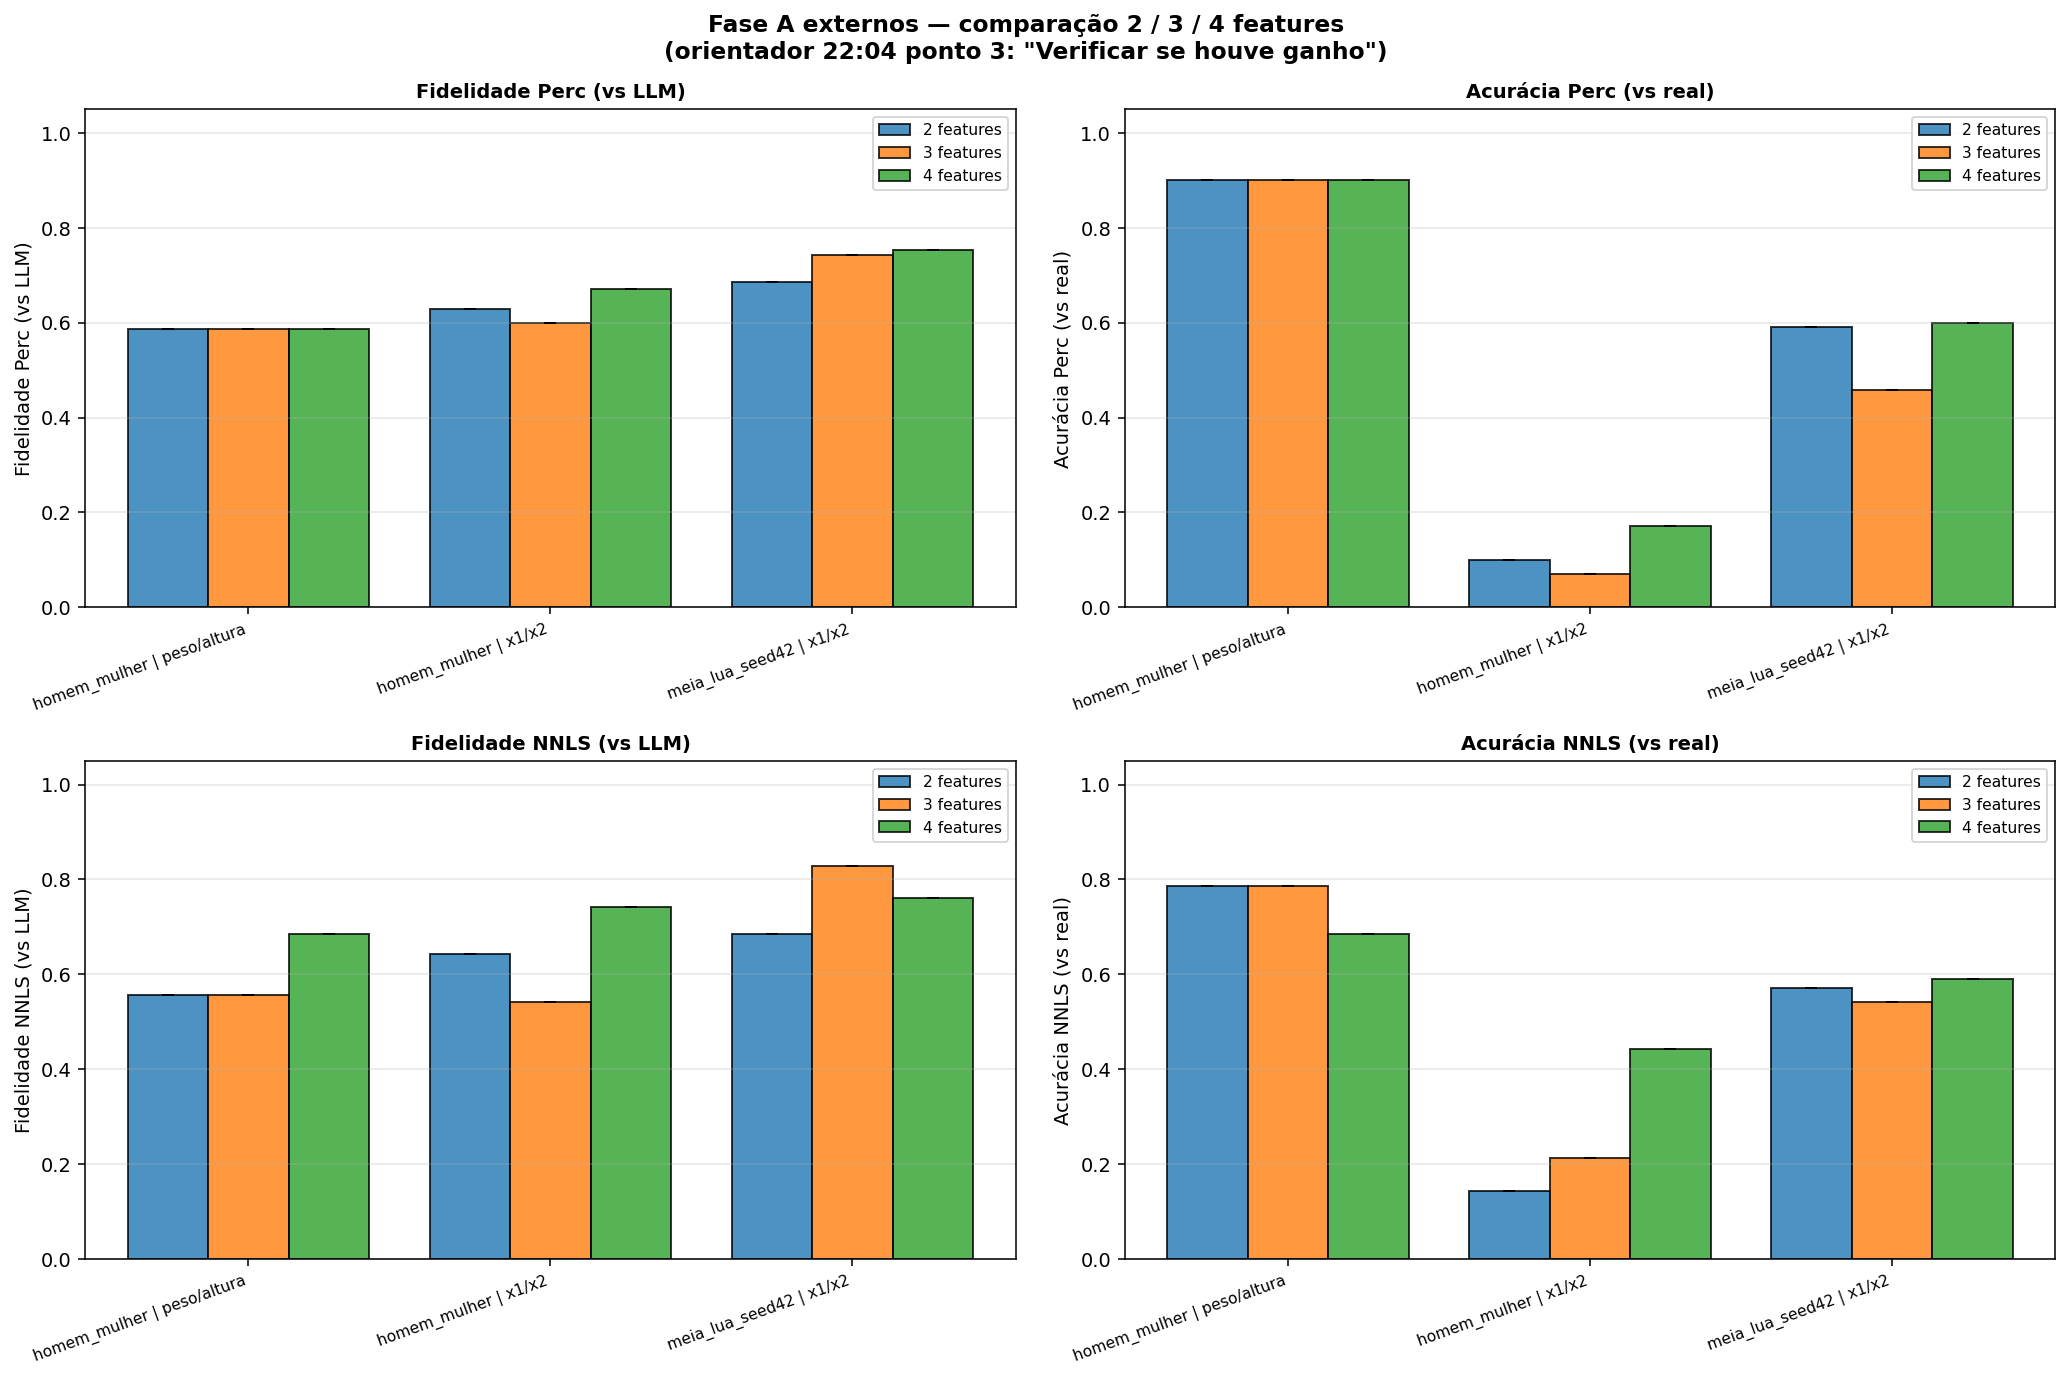
\includegraphics[width=0.85\linewidth,height=0.6\textheight,keepaspectratio]{bloco23_external_features_comparison.png}
  \end{center}
  \textbf{Contraste com slide 23:} aqui esperamos GANHO (problema genuinamente n\~ao-linear).
\end{frame}

% 25 - Meta-teste transferencia
\begin{frame}{Transfer\^encia de $W$ em R4 --- meia-lua $\to$ A/B/C}
  \scriptsize
  \textbf{Meta-teste cruzado:} aprende $W$ em R4 na meia-lua; aplica em A, B, C augmentados para R4. Esperado: queda forte --- a m\'etrica \'e espec\'ifica do problema.
  \medskip
  \begin{center}
    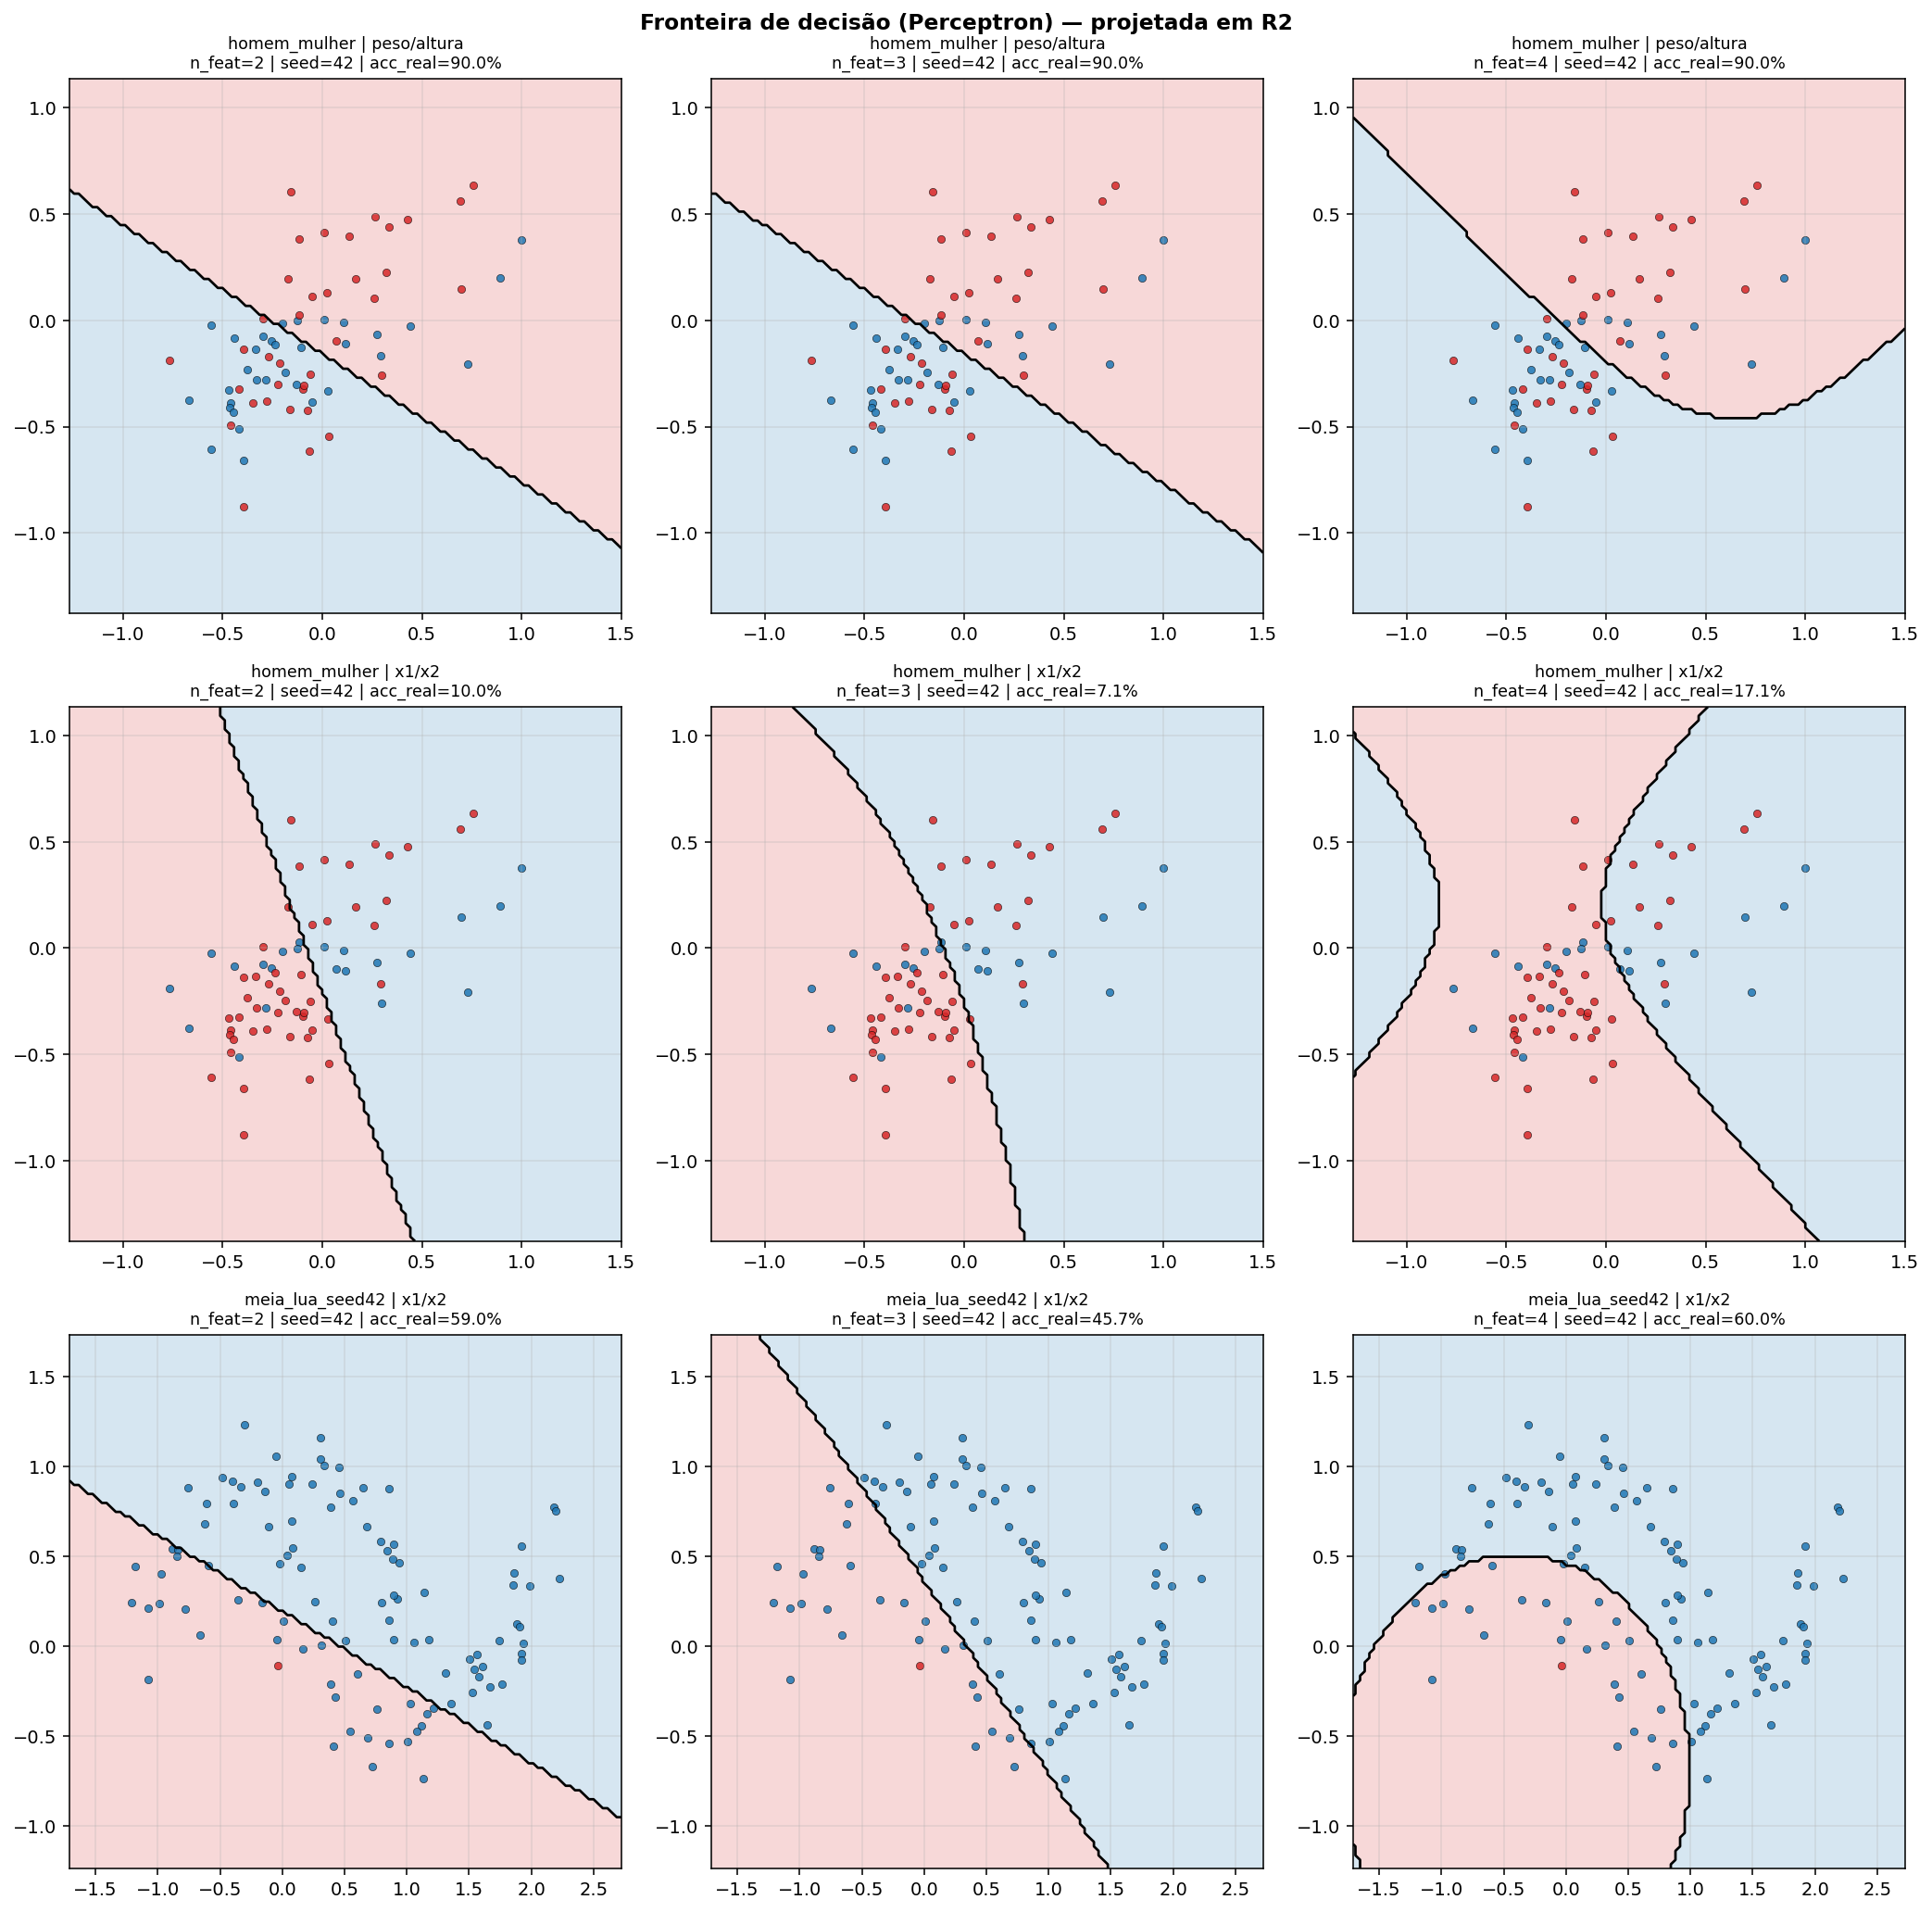
\includegraphics[width=0.55\linewidth,height=0.55\textheight,keepaspectratio]{bloco23_external_decision_boundary.png}
  \end{center}
  Fronteiras de decis\~ao das m\'etricas externas projetadas em R2.
\end{frame}

% 26 - Sintese R2/R3/R4
\begin{frame}{S\'intese R2 / R3 / R4 do Bloco 1}
  \scriptsize
  \begin{center}
  \begin{tabular}{lcc}
    \toprule
    Problema & $\Delta$ R2$\to$R4 acc\_real & Esperado \\
    \midrule
    A/B/C lineares & $\sim 0$ p.p.\           & sem ganho $\checkmark$ \\
    D meia-lua     & \textbf{positivo}        & ganho $\checkmark$ \\
    \bottomrule
  \end{tabular}
  \end{center}
  \medskip
  \textbf{Mensagem:} R3/R4 ajuda APENAS em problemas n\~ao-lineares. Em A/B/C lineares, adicionar features \'e overfitting silencioso.
\end{frame}

% 27 - Vies de ordem
\begin{frame}{Vi\'es de ordem das classes}
  \scriptsize
  \begin{center}
    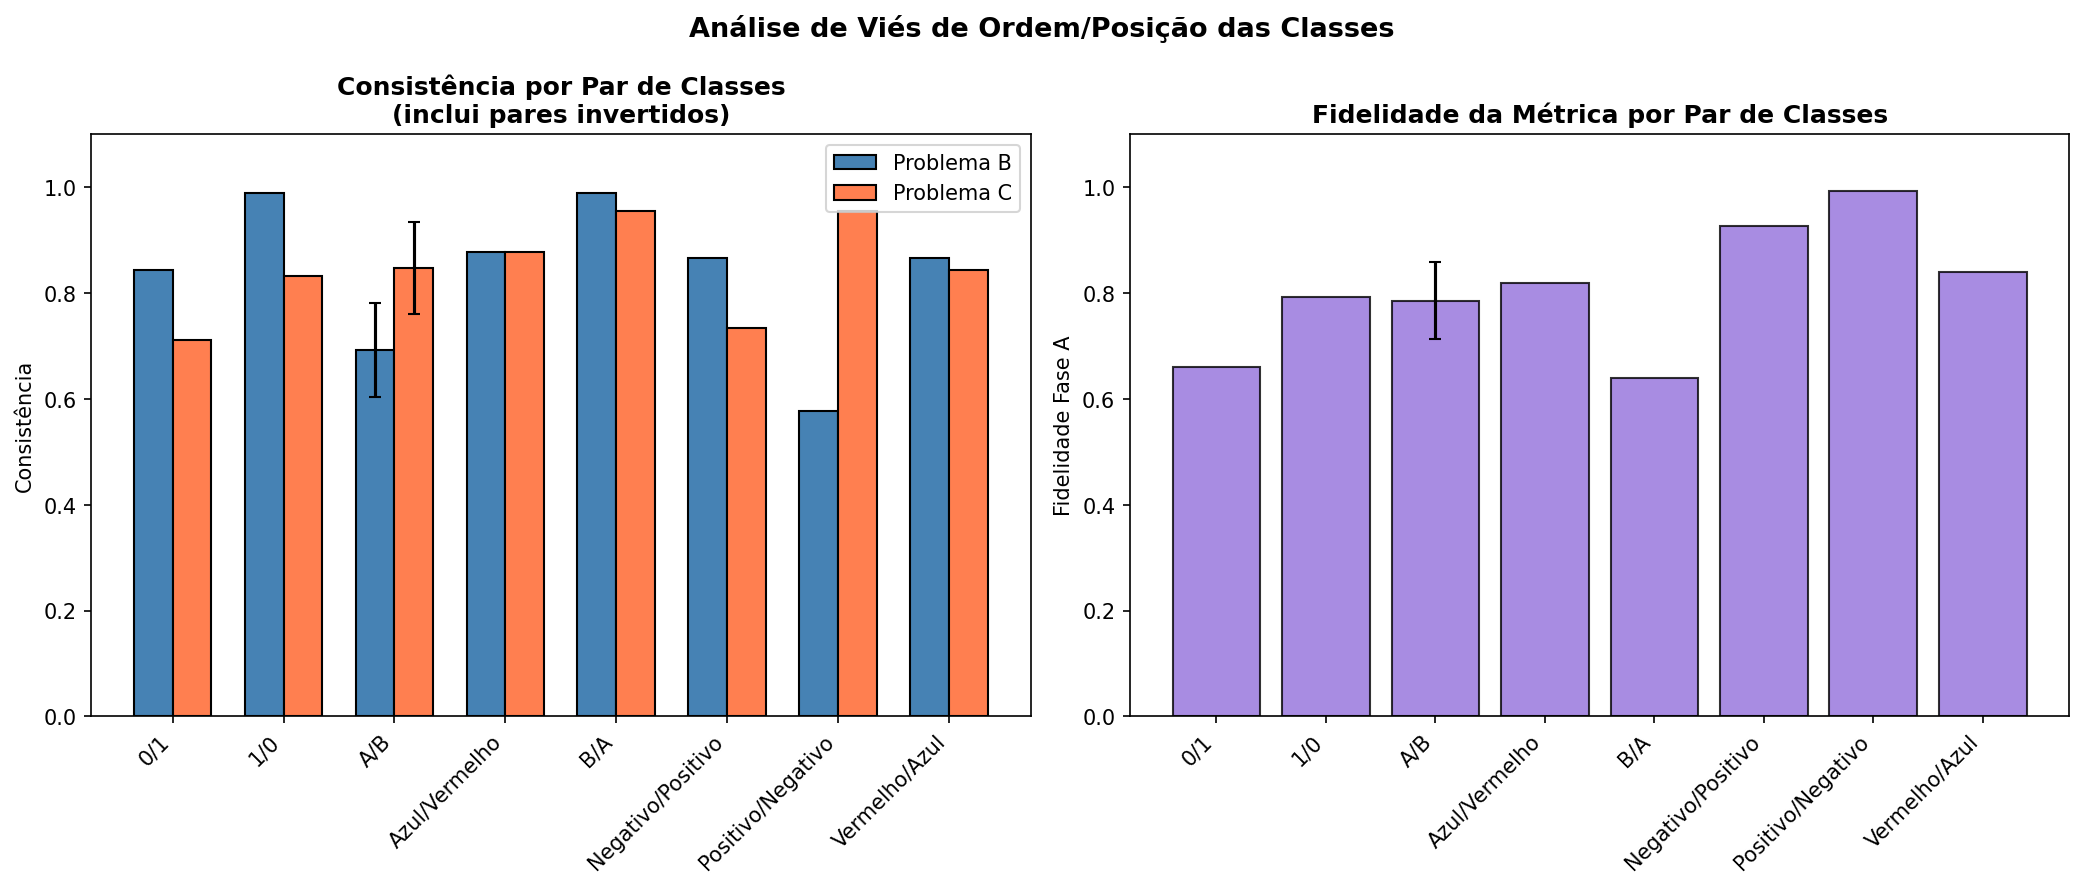
\includegraphics[width=0.8\linewidth,height=0.7\textheight,keepaspectratio]{bloco1_12_class_order_bias.png}
  \end{center}
  Compara pares A/B vs B/A, 0/1 vs 1/0, Pos/Neg vs Neg/Pos. Vi\'es marginal nesta execu\c{c}\~ao.
\end{frame}

% 28 - Variantes de prompt + nomes
\begin{frame}{Variantes de prompt + nomes sem\^anticos}
  \scriptsize
  \begin{columns}[T]
    \column{0.5\linewidth}
    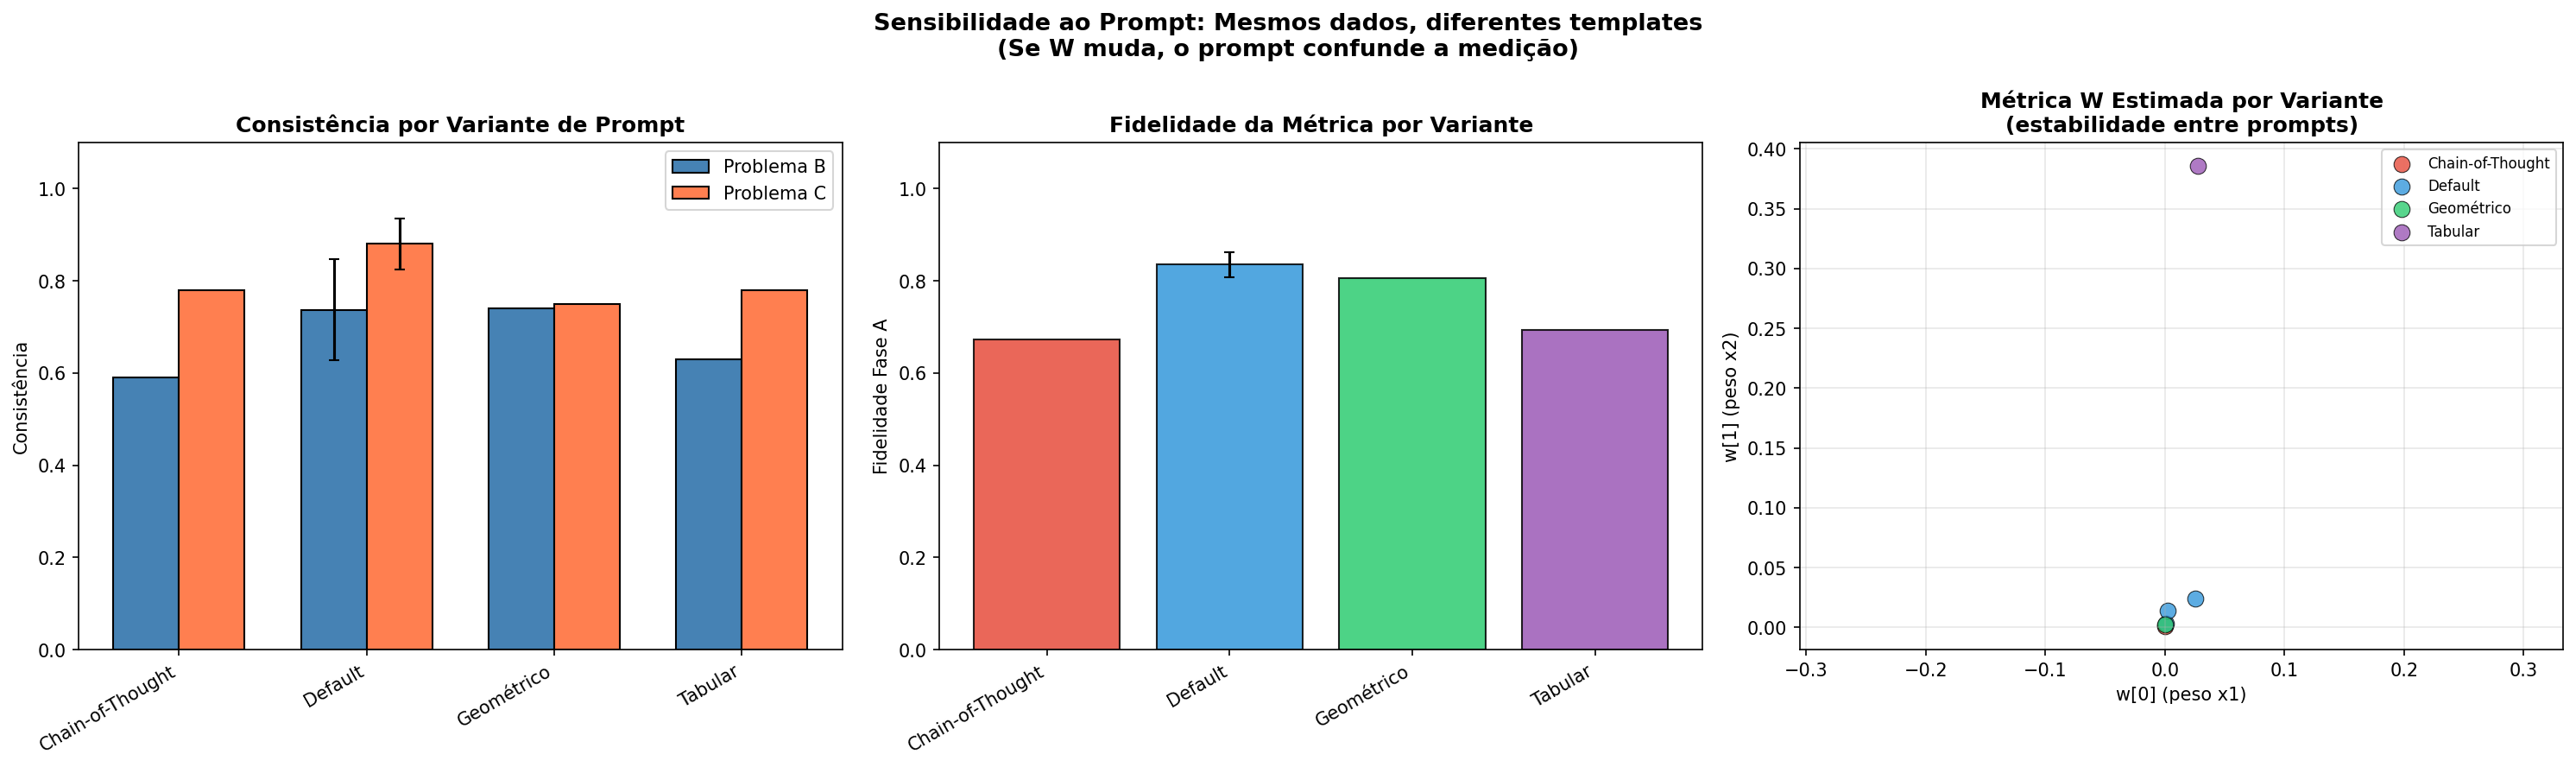
\includegraphics[width=\linewidth,height=0.6\textheight,keepaspectratio]{bloco1_13_prompt_variants.png}
    \column{0.5\linewidth}
    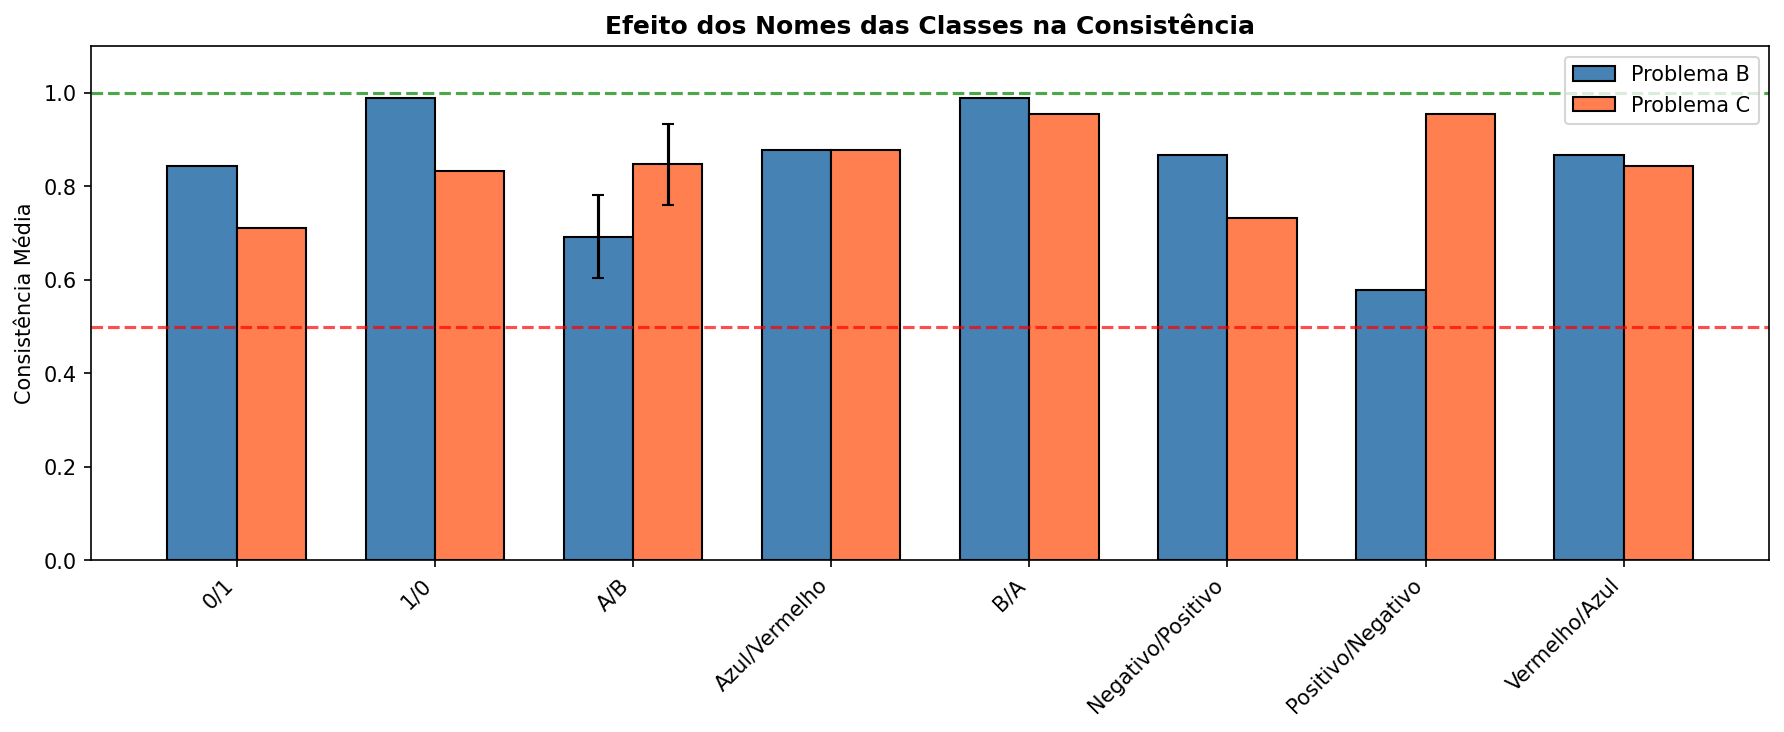
\includegraphics[width=\linewidth,height=0.3\textheight,keepaspectratio]{bloco1_14a_class_names_effect.png}
    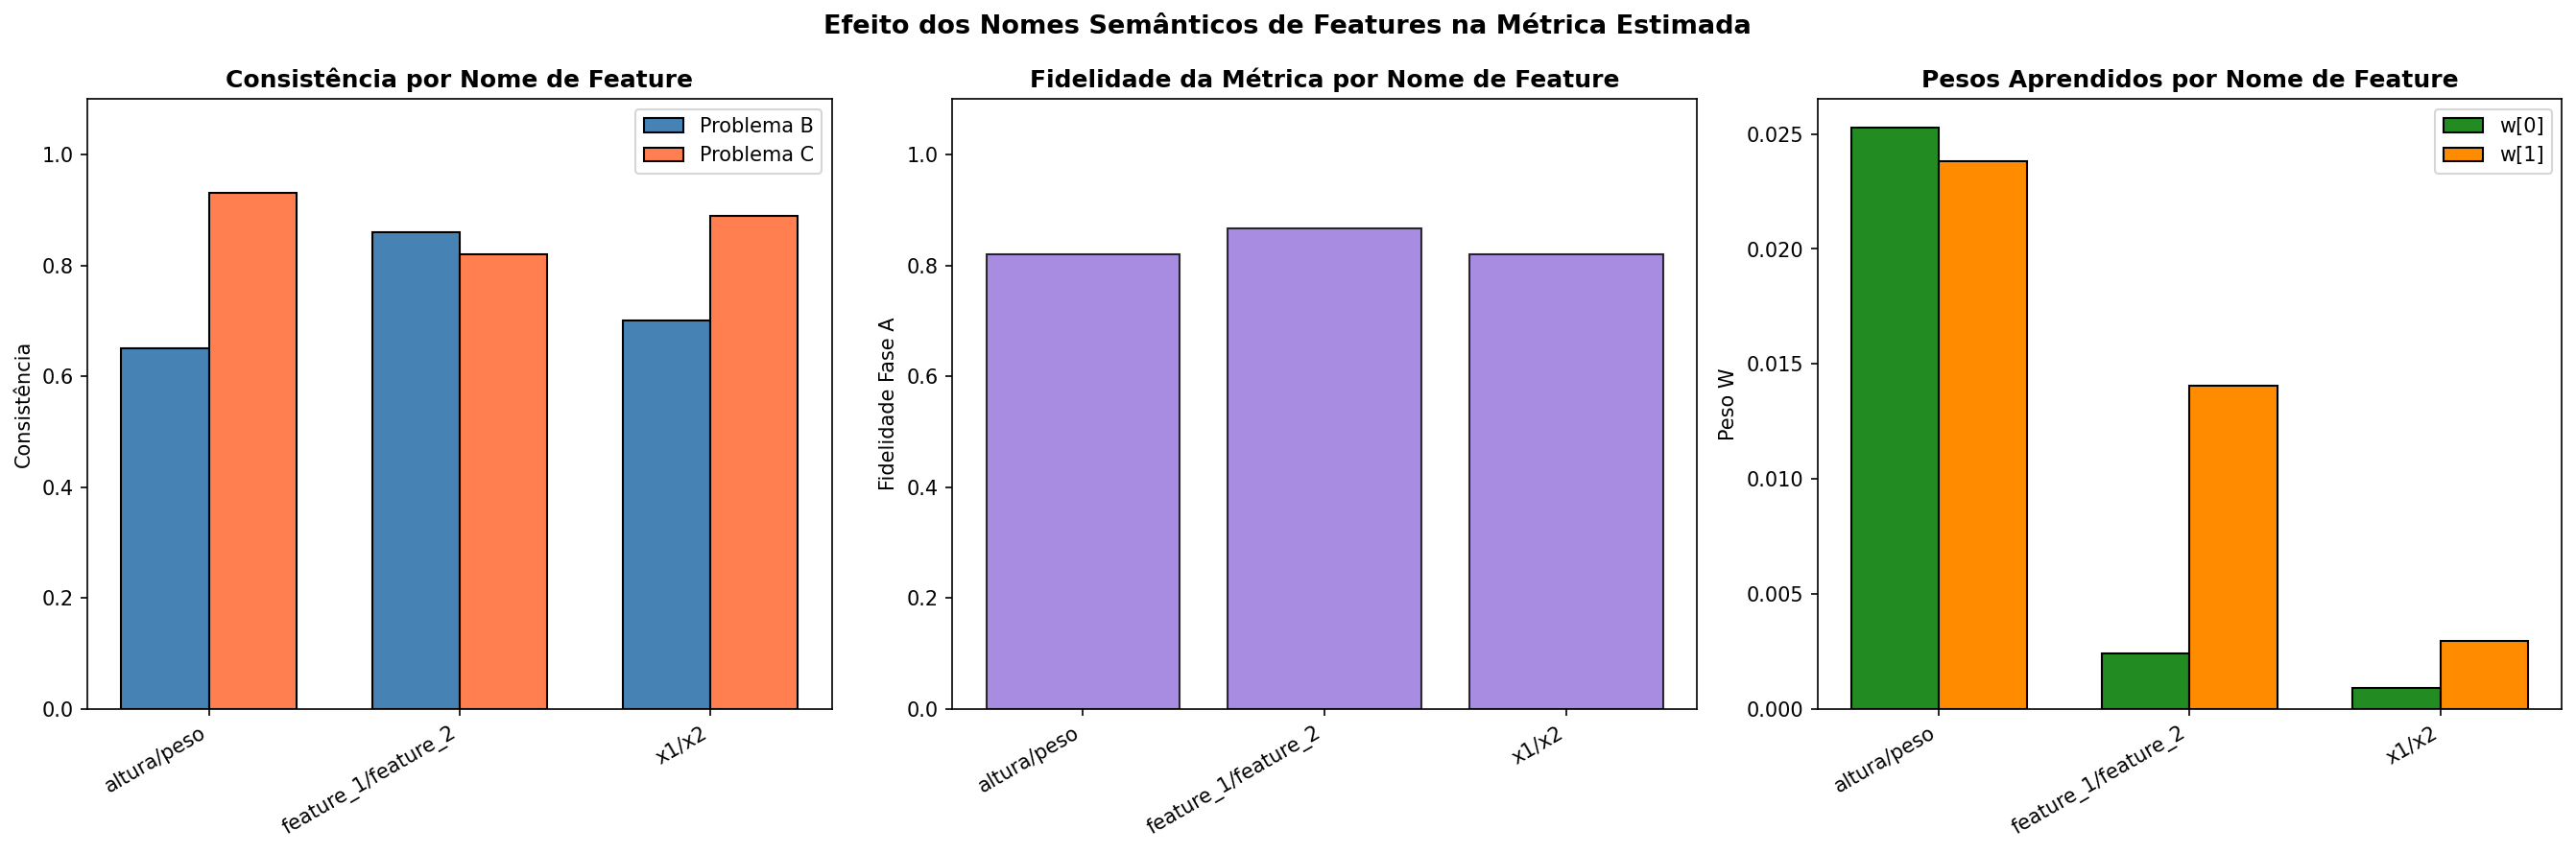
\includegraphics[width=\linewidth,height=0.3\textheight,keepaspectratio]{bloco1_14b_feature_names_effect.png}
  \end{columns}
  \medskip
  4 variantes (default, geometric, cot, tabular) + 3 conjuntos de nomes (x1/x2, altura/peso, feature\_1/feature\_2).
\end{frame}

% 29 - Prompts literais 1/2
\begin{frame}[fragile]{Prompts literais (1/2) --- default zero-shot e few-shot}
  \tiny
  \textbf{Zero-shot} (\texttt{build\_prompt\_zero\_shot}):
  \begin{verbatim}
Considere o problema de classificar pontos 2D em duas classes (A ou B).
Dado o ponto (x1=1.234, x2=-0.567), responda apenas com a letra da classe.
Responda: A ou B.
  \end{verbatim}
  \textbf{Few-shot} (5 exemplos):
  \begin{verbatim}
Voce vera 5 exemplos rotulados e depois um ponto a classificar.
Exemplo 1: (x1=-2.3, x2=0.1) -> A
Exemplo 2: (x1=2.1, x2=-0.2) -> B
...
Agora classifique: (x1=0.234, x2=0.567)
Responda apenas: A ou B.
  \end{verbatim}
\end{frame}

% 30 - Prompts literais 2/2
\begin{frame}[fragile]{Prompts literais (2/2) --- variantes}
  \tiny
  \textbf{Geometric:} \texttt{Voce ve dois grupos de pontos em um plano cartesiano...}\\
  \textbf{CoT:} \texttt{Pense passo a passo: 1) Localize o ponto, 2) Compare com exemplos, 3) Decida...}\\
  \textbf{Tabular:}
  \begin{verbatim}
| x1   | x2    | classe |
|------|-------|--------|
| -2.3 | 0.1   | A      |
| 2.1  | -0.2  | B      |
| 1.234| -0.567| ?      |
  \end{verbatim}
  Todas as variantes terminam com a mesma instru\c{c}\~ao final ("\emph{responda apenas A ou B}").
\end{frame}

% 31 - Resumo Bloco 1
\begin{frame}{Resumo Bloco 1}
  \footnotesize
  \begin{itemize}
    \item \textbf{H1 SUSTENTADA}: Kappa C = $0{,}77$--$0{,}81$ (Perceptron/NNLS); Kappa B mais modesto ($0{,}29$--$0{,}33$) com rota\c{c}\~ao agressiva $\pm 1{,}5$.
    \item \textbf{Fidelidade Fase A}: 82--83\% --- a m\'etrica reproduz quatro em cinco decis\~oes.
    \item \textbf{Algoritmos congruentes}: Perceptron e NNLS chegam ao mesmo $W$.
    \item \textbf{R3/R4} s\'o ajuda em D meia-lua (preview do Bloco 2/3).
    \item \textbf{Vieses} de prompt e ordem de classes s\~ao marginais nesta execu\c{c}\~ao.
  \end{itemize}
\end{frame}

% ===== BLOCO 2 =====
\begin{frame}{Bloco 2 --- LLM como APRENDIZ (Fase E)}
  \footnotesize
  \begin{center}\Large\textbf{Bloco 2 --- LLM como APRENDIZ}\end{center}
  \medskip
  \begin{itemize}
    \item Perito externo \textbf{rotula}; LLM \textbf{aprende} via in-context learning (Fase E).
    \item Problemas: \textbf{E} (linear, antigo D, $W_{\text{expert}}=[0{,}3;\ 1{,}5]$) e \textbf{F} (meia-lua, perito = ground truth).
    \item Hip\'oteses: \textbf{H3} (LLM como aprendiz), \textbf{H4} (exemplos dif\'iceis), \textbf{H5}.
  \end{itemize}
\end{frame}

% 33 - Visao geral B2
\begin{frame}{Vis\~ao geral dos 2 problemas do Bloco 2}
  \scriptsize
  \begin{columns}[T]
    \column{0.5\linewidth}
    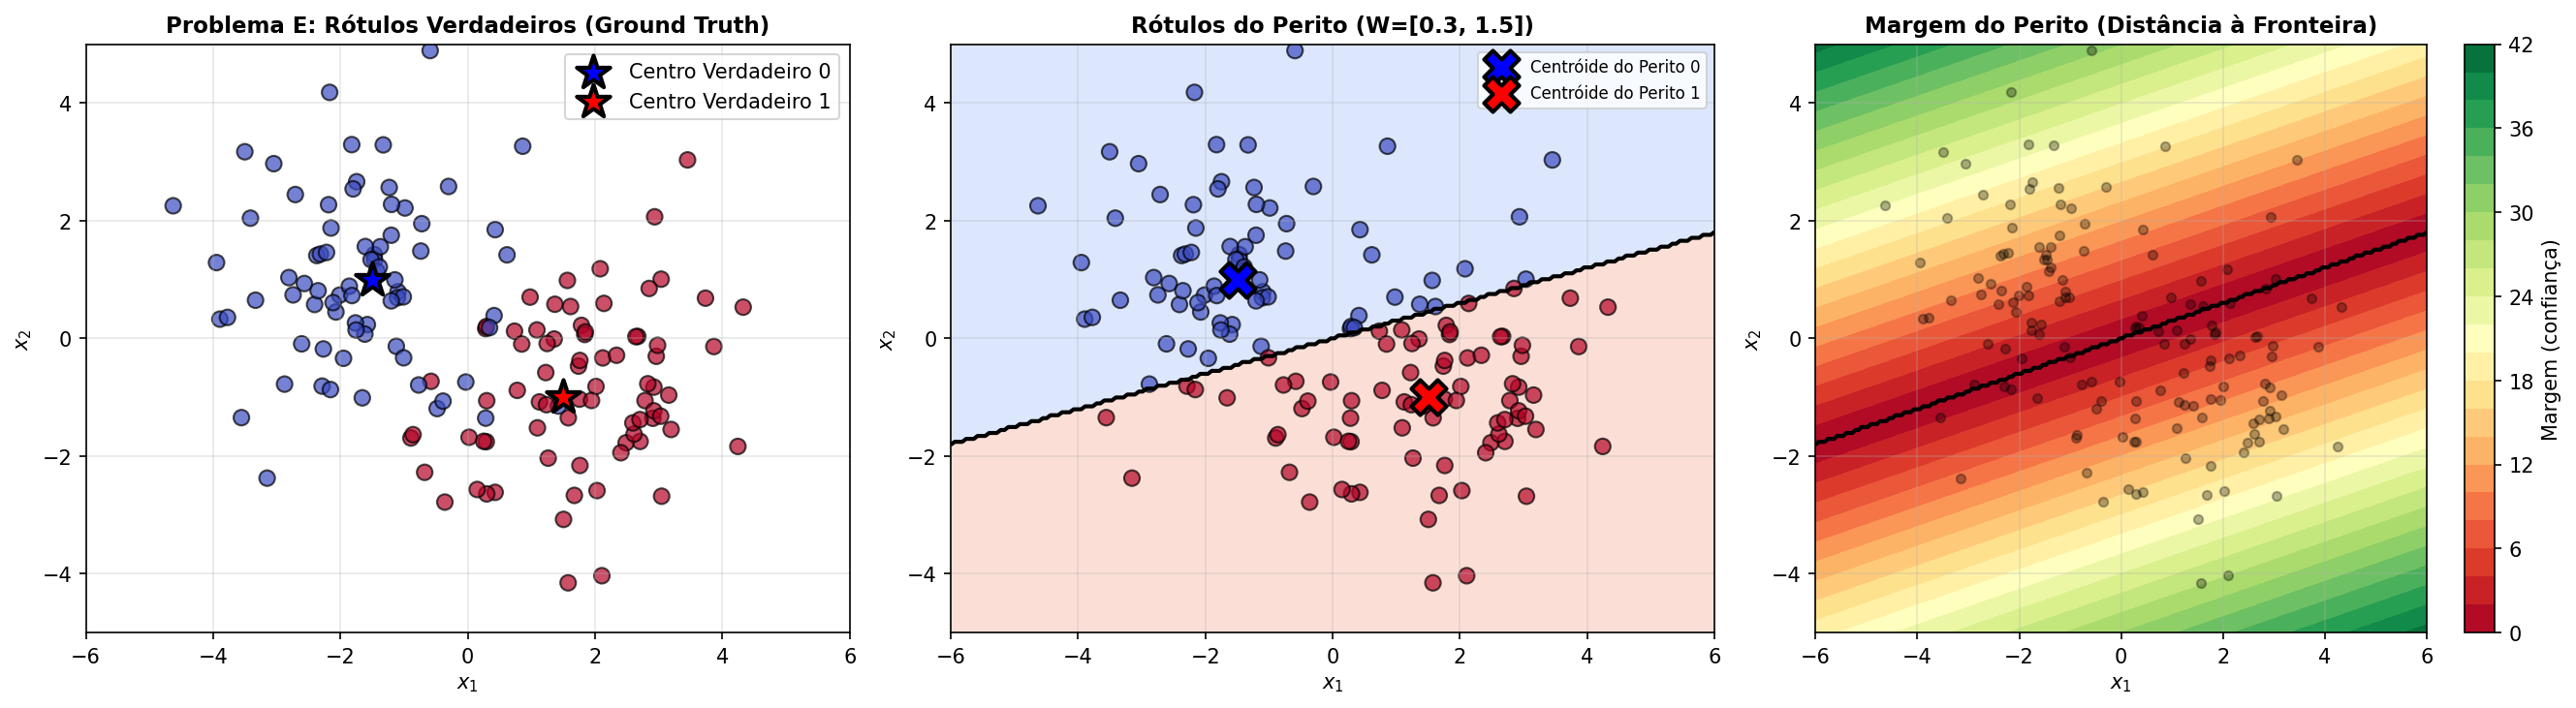
\includegraphics[width=\linewidth,height=0.7\textheight,keepaspectratio]{bloco2_01_problema_e_expert.png}
    \column{0.5\linewidth}
    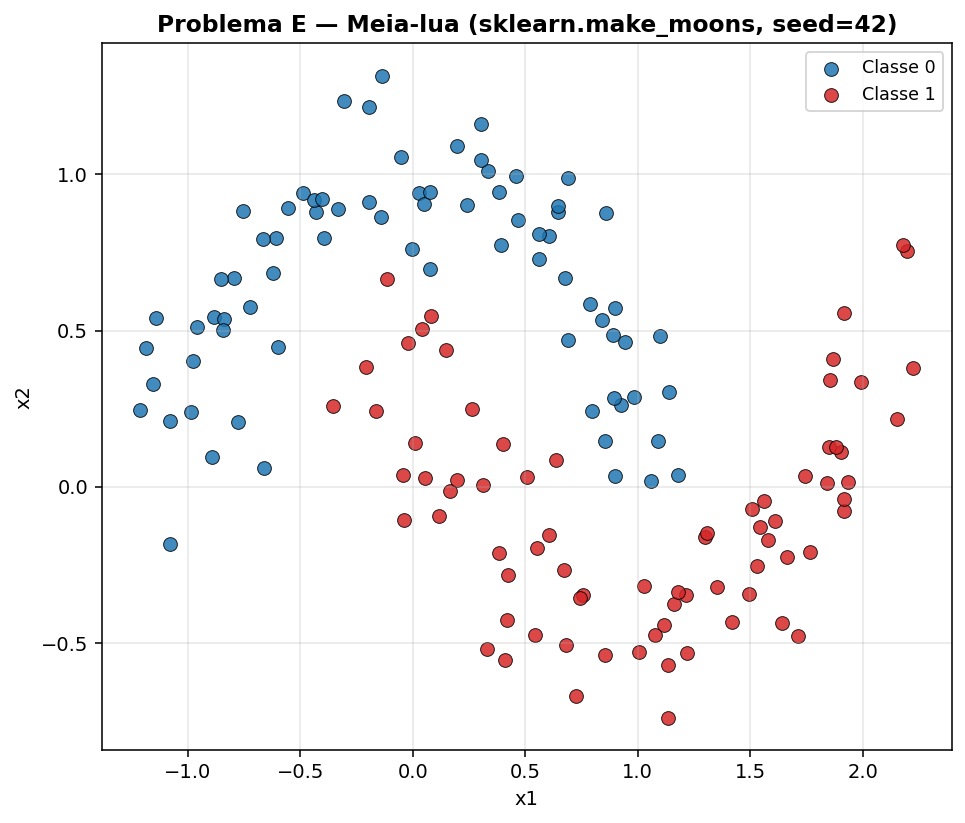
\includegraphics[width=\linewidth,height=0.7\textheight,keepaspectratio]{bloco1_02_problema_d_meialua_seed42_overview.png}
  \end{columns}
\end{frame}

% 34 - Problema E
\begin{frame}{Problema E --- perito linear (antigo D)}
  \scriptsize
  \begin{columns}[T]
    \column{0.55\linewidth}
    \textbf{Prop\'osito:} pap\'eis invertidos. Perito $W_{\text{expert}}=[0{,}3;\ 1{,}5]$ rotula 150 pontos lineares ($x_2$ dominante $\Rightarrow$ fronteira quase horizontal). LLM tenta reproduzir via few-shot.
    \medskip

    Parametros:
    \begin{itemize}
      \item Centr\'oides $(-1{,}5; +1)$ e $(1{,}5; -1)$
      \item \texttt{cluster\_std}=1{,}3, $n=150$
      \item R\'otulos via $W_{\text{expert}}$ ($\arg\min_k d_W$).
    \end{itemize}
    \column{0.45\linewidth}
    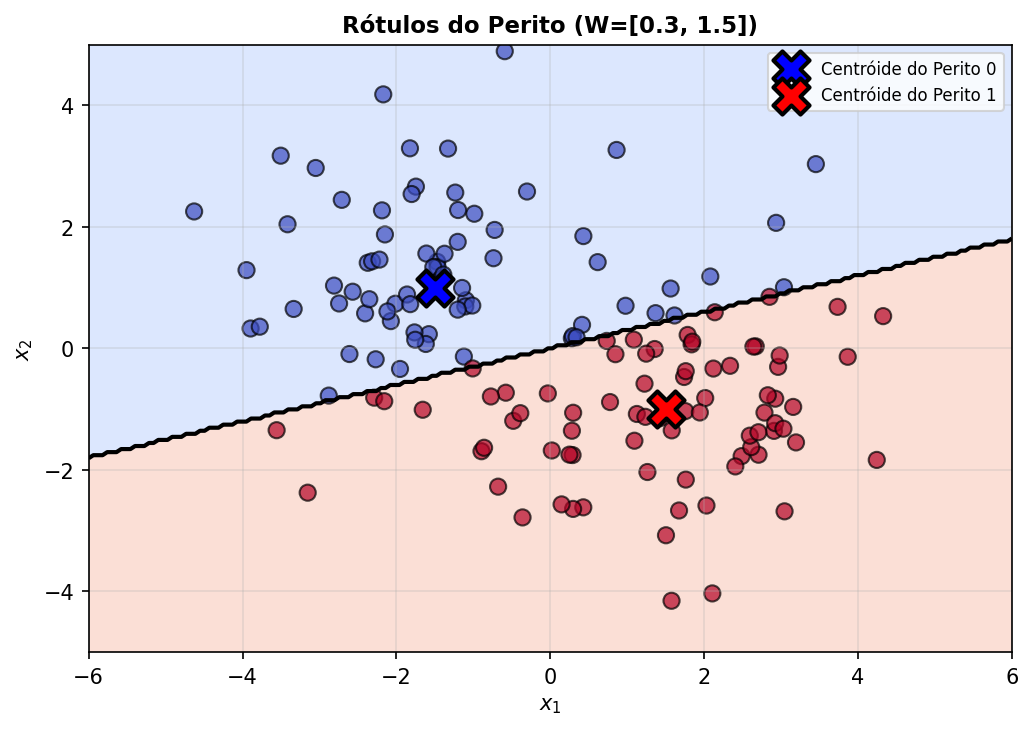
\includegraphics[width=\linewidth,height=0.65\textheight,keepaspectratio]{bloco2_01_problema_e_expert_fronteira_perito.png}
  \end{columns}
\end{frame}

% 35 - Problema F meia-lua
\begin{frame}{Problema F --- meia-lua com perito = ground truth}
  \scriptsize
  \begin{columns}[T]
    \column{0.55\linewidth}
    \textbf{Prop\'osito:} regime n\~ao-linear genuino. O perito \'e o pr\'oprio \texttt{make\_moons} (ground truth). LLM precisa capturar a fronteira em S apenas pelos exemplos.
    \medskip

    \textbf{Por qu\^e:} testa H3 em regime n\~ao-linear. LLM recebe apenas $(x_1, x_2)$ --- nem augmenta\c{c}\~ao R3 nem R4 no prompt.
    \column{0.45\linewidth}
    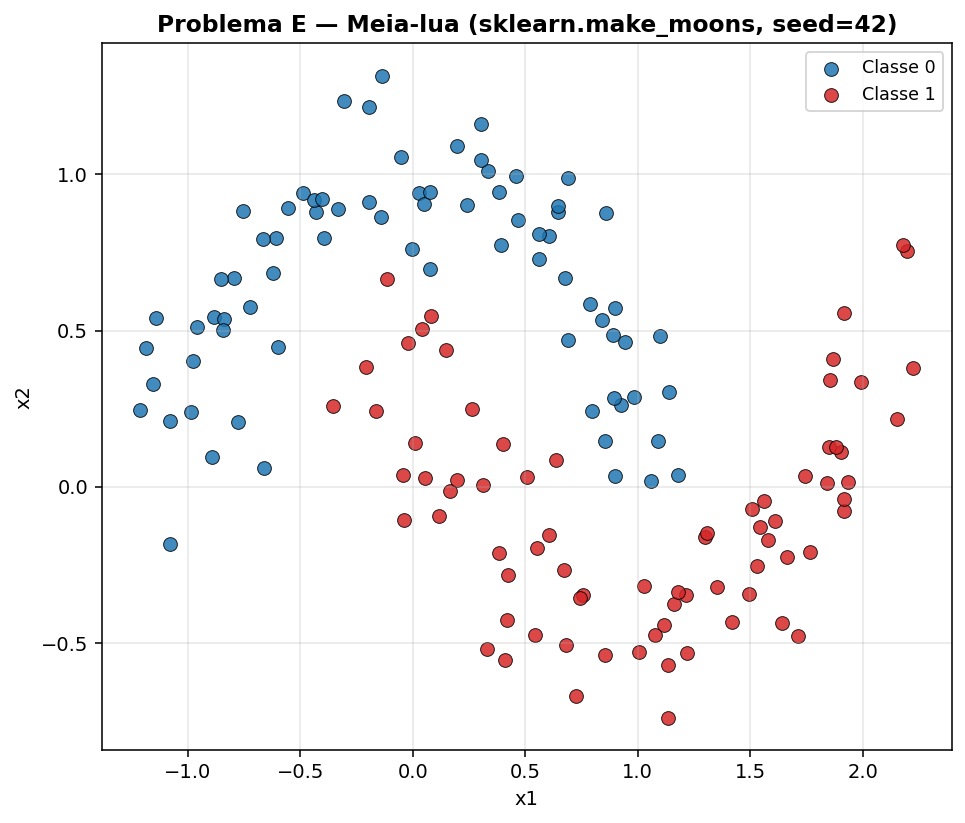
\includegraphics[width=\linewidth,height=0.7\textheight,keepaspectratio]{bloco1_02_problema_d_meialua_seed42_overview.png}
  \end{columns}
\end{frame}

% 36 - Fase E descricao
\begin{frame}{Fase E --- LLM como aprendiz (passo a passo)}
  \scriptsize
  \begin{enumerate}
    \item Perito rotula os 150 pontos do Problema E (ou ground truth no F).
    \item Divide em treino/teste.
    \item Para cada $n_{\text{shot}} \in \{0, 5\}$ (smoke; produ\c{c}\~ao at\'e 40): seleciona exemplos via estrat\'egia.
    \item Envia exemplos + ponto de teste em prompt few-shot.
    \item Mede acur\'acia, Kappa, F1 do LLM vs r\'otulos do perito.
  \end{enumerate}
\end{frame}

% 37 - Estrategias
\begin{frame}{Estrat\'egias de sele\c{c}\~ao de exemplos}
  \scriptsize
  \begin{center}
    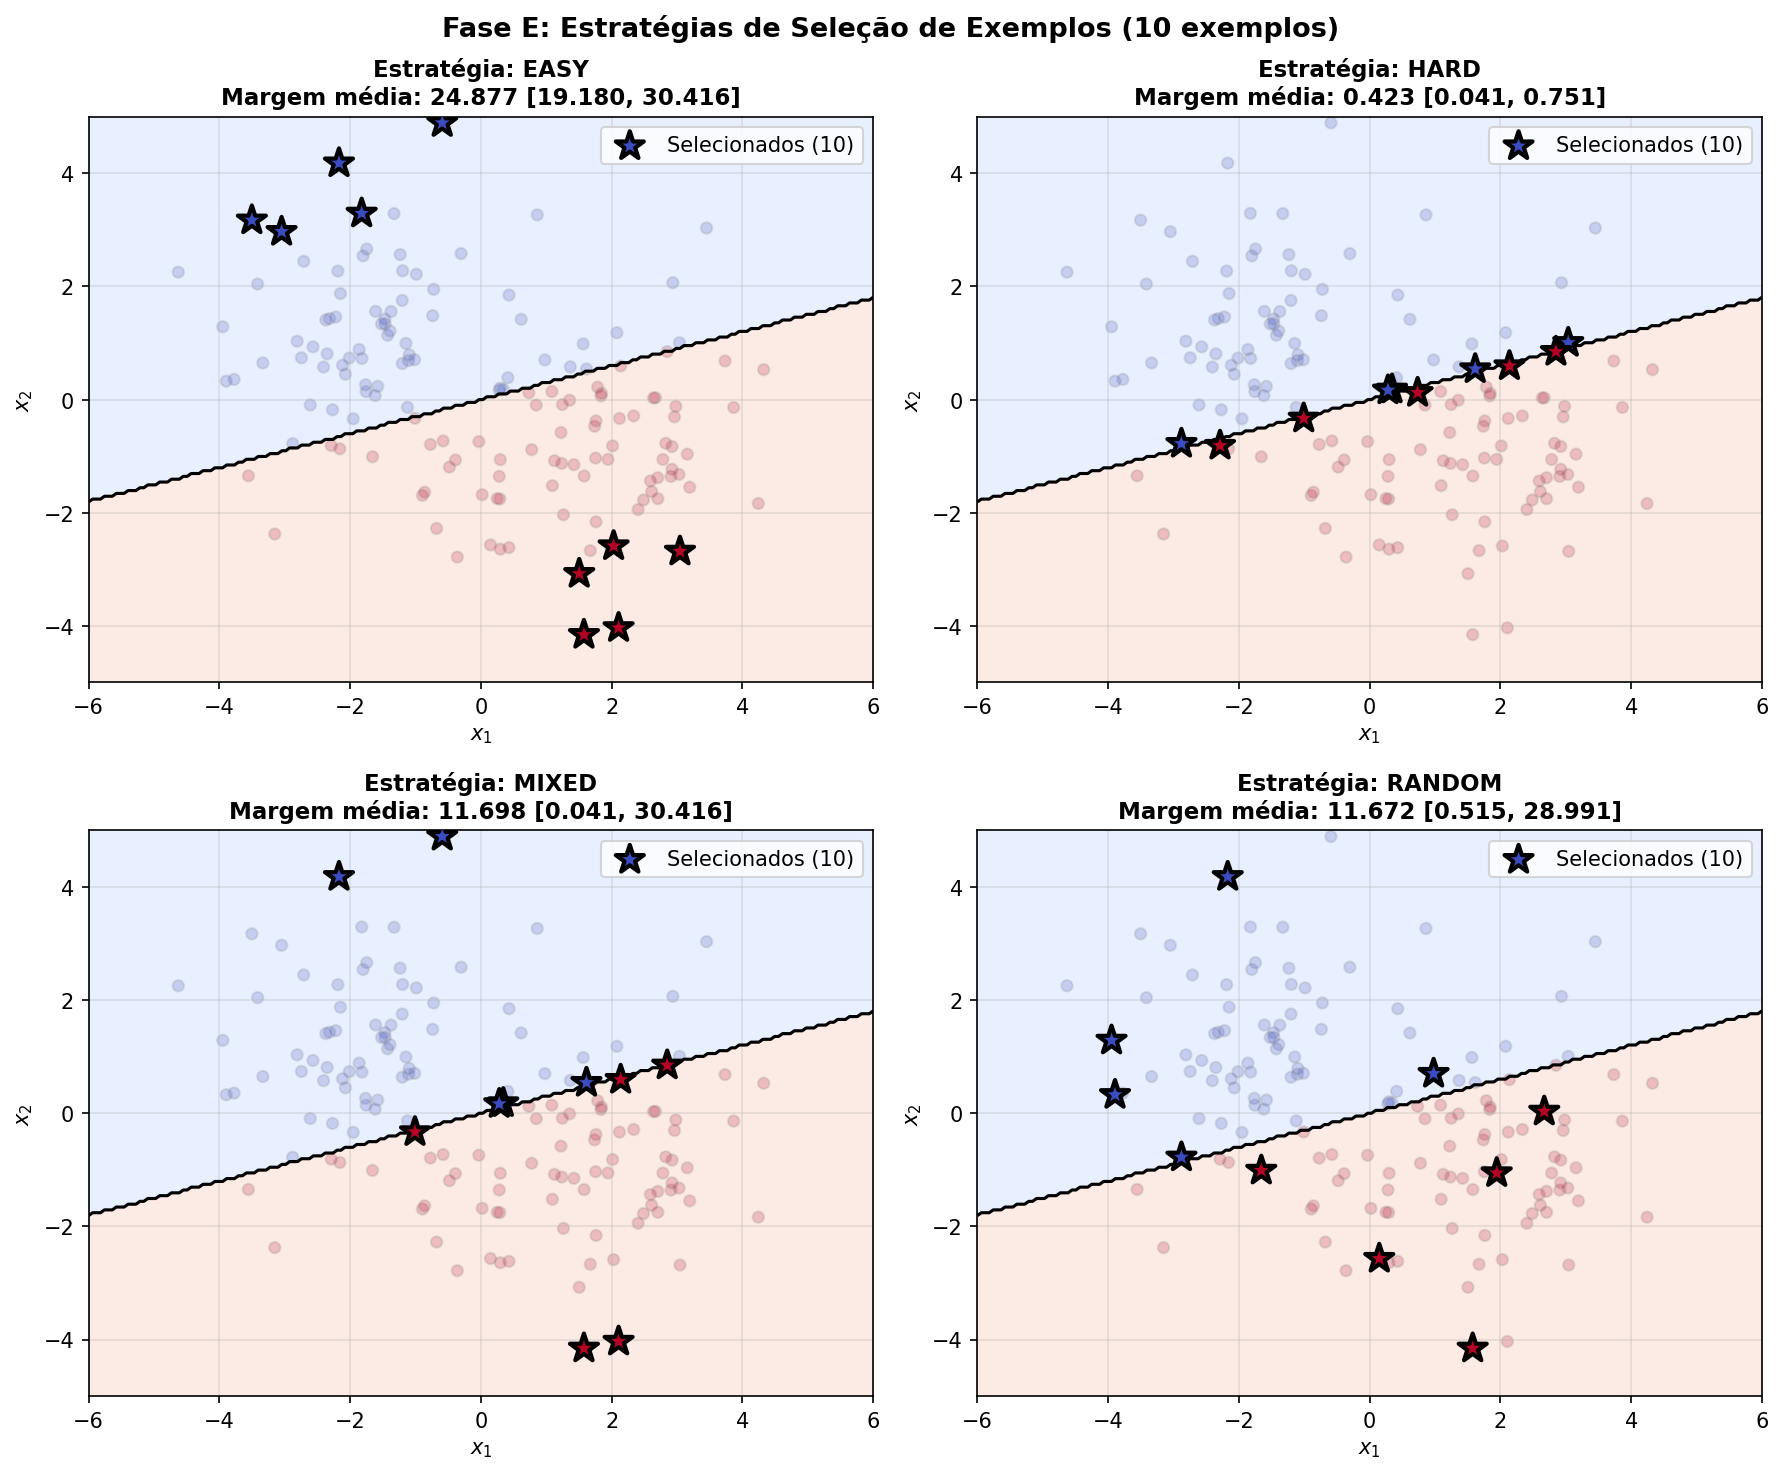
\includegraphics[width=0.85\linewidth,height=0.75\textheight,keepaspectratio]{bloco2_03_phase_e_strategies.png}
  \end{center}
  \textbf{easy}: alta margem. \textbf{hard}: pr\'oximos da fronteira. \textbf{mixed}: 50/50. \textbf{random}: baseline.
\end{frame}

% 38 - Curvas de aprendizado
\begin{frame}{Fase E --- curvas de aprendizado}
  \scriptsize
  \begin{center}
    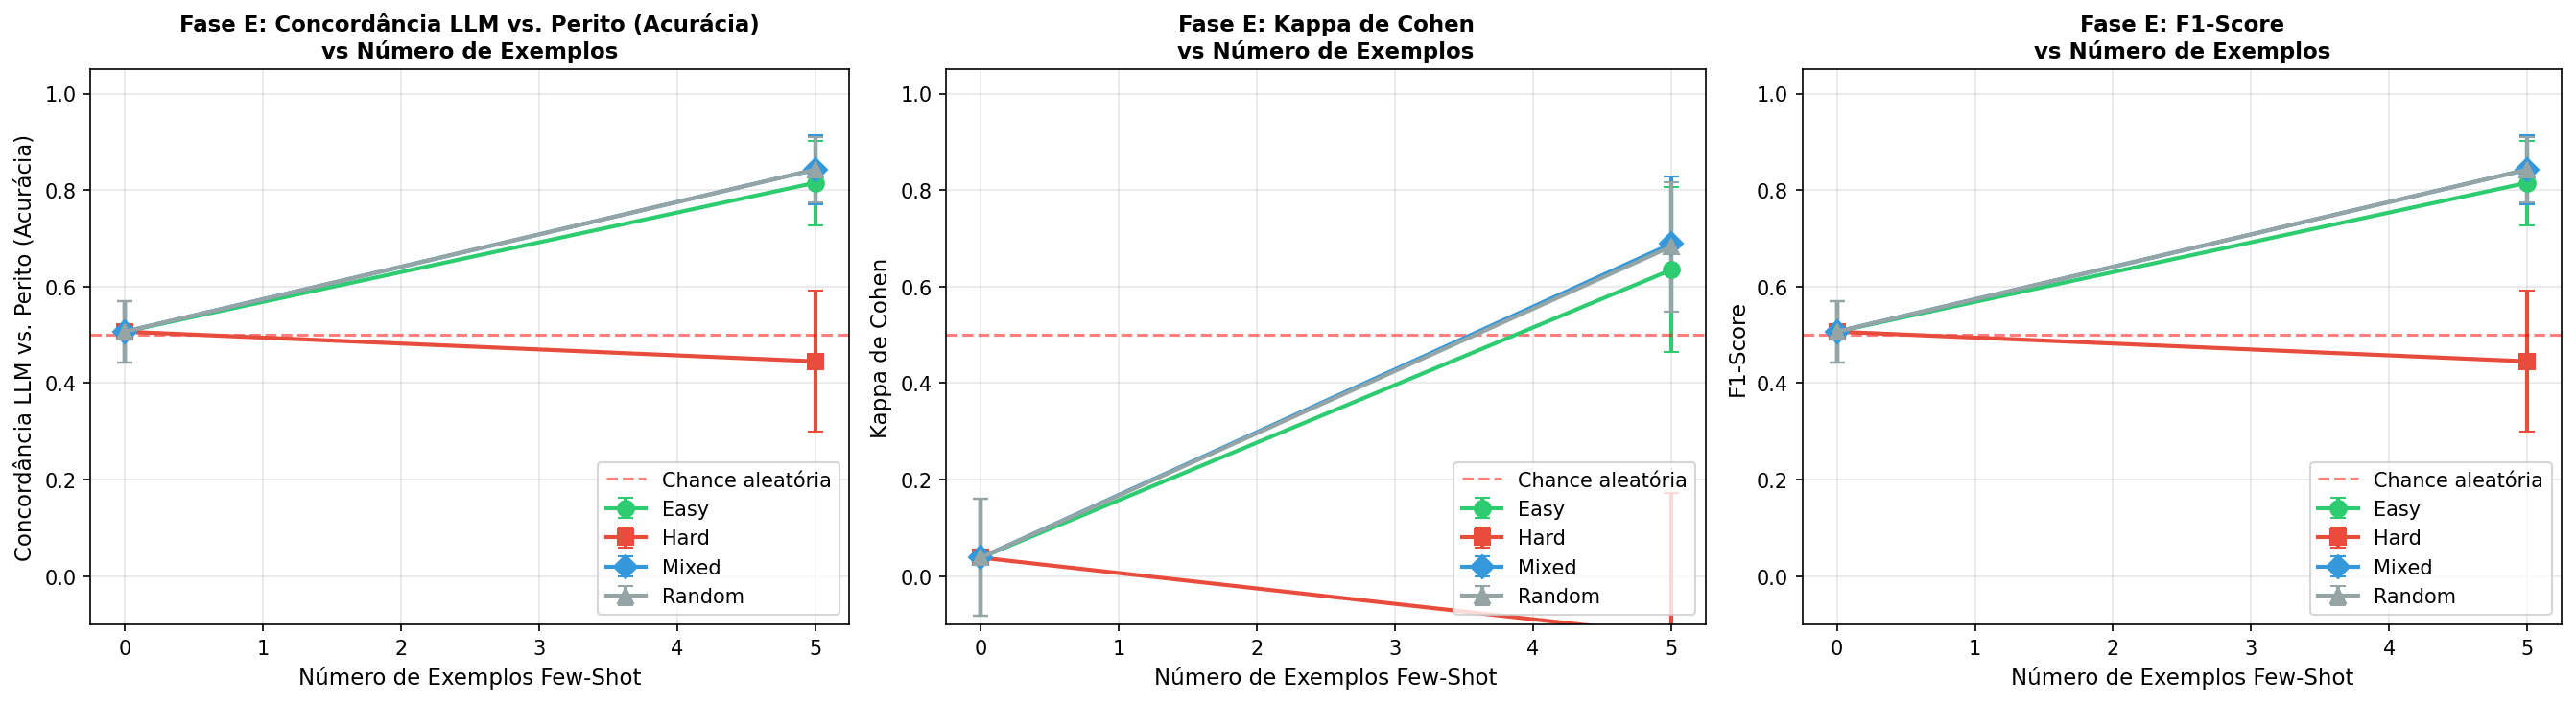
\includegraphics[width=0.85\linewidth,height=0.75\textheight,keepaspectratio]{bloco2_04_phase_e_learning_curve.png}
  \end{center}
  Smoke run com $n_{\text{shot}}\in\{0, 5\}$. Em produ\c{c}\~ao at\'e 40 mostra plateau cl\'assico do in-context learning.
\end{frame}

% 39 - Estrategia comparison
\begin{frame}{Fase E --- compara\c{c}\~ao de estrat\'egias (refuta\c{c}\~ao H4)}
  \scriptsize
  \begin{center}
    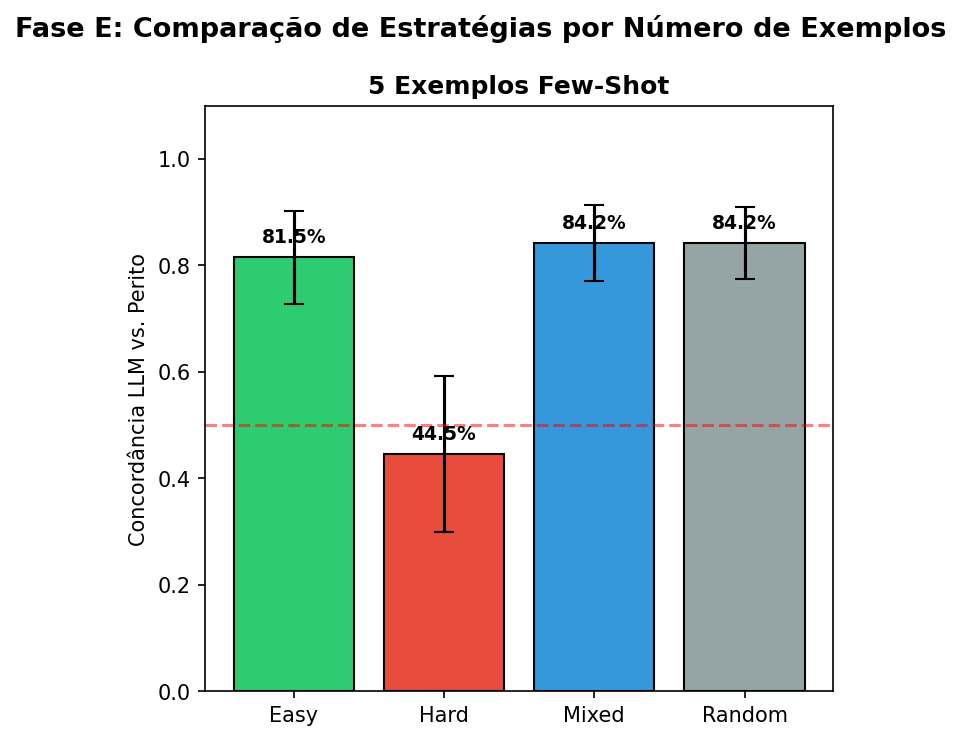
\includegraphics[width=0.85\linewidth,height=0.75\textheight,keepaspectratio]{bloco2_05_phase_e_strategy_comparison.png}
  \end{center}
  Mesmo no smoke (5-shot), \emph{easy} aparece \`a frente. Em produ\c{c}\~ao, refuta\c{c}\~ao com Cohen $d \sim 1{,}5$.
\end{frame}

% 40 - Refutacao H4
\begin{frame}{Refuta\c{c}\~ao de H4 --- intui\c{c}\~ao}
  \footnotesize
  Hip\'otese a priori: exemplos amb\'iguos (\emph{hard}) ensinam mais (active learning).
  \medskip

  \textbf{Achado:} em LLMs in-context, exemplos prototipicos (\emph{easy}, alta margem) funcionam como \textbf{\^ancoras de classe}:
  \begin{itemize}
    \item Hard $\to$ sinal contradit\'orio (sem gradiente, n\~ao h\'a como extrair informa\c{c}\~ao da ambig\"uidade).
    \item Easy $\to$ pivots claros para o LLM aprender "look-and-feel" de cada classe.
  \end{itemize}
  \medskip

  Conex\~ao com Lyu et al.\ (2023): prompts can\^onicos batem amb\'iguos.
\end{frame}

% 41 - Multiplos experts
\begin{frame}{M\'ultiplos experts (smoke; produ\c{c}\~ao tem 3 seeds $\times$ 3 reps)}
  \scriptsize
  \begin{center}
  \begin{tabular}{lcc}
    \toprule
    Expert & $W$ & Acur\'acia LLM 5-shot \\
    \midrule
    \texttt{aniso\_x2}   & $[0{,}3, 1{,}5]$ & \emph{ver CSV} \\
    \texttt{aniso\_x1}   & $[1{,}5, 0{,}3]$ & \emph{ver CSV} \\
    \texttt{euclidean}   & $[1{,}0, 1{,}0]$ & \emph{ver CSV} \\
    \bottomrule
  \end{tabular}
  \end{center}
  Dados completos em \texttt{bloco2\_phase\_e\_20260514\_175854.csv}. LLM aprende todos com efic\'acia variada --- Euclidean costuma liderar.
\end{frame}

% 42 - Diluicao
\begin{frame}{Experimento de dilui\c{c}\~ao}
  \scriptsize
  \begin{columns}[T]
    \column{0.45\linewidth}
    Design: 4 \emph{hard} fixos + adicionar \emph{easy} progressivamente.
    \medskip

    \textbf{Pergunta:} \emph{easy} dilui o sinal dos \emph{hard}?
    \medskip

    \textbf{Achado em produ\c{c}\~ao:} curva monot\^onica crescente --- \emph{easy} ajuda sempre.
    \column{0.55\linewidth}
    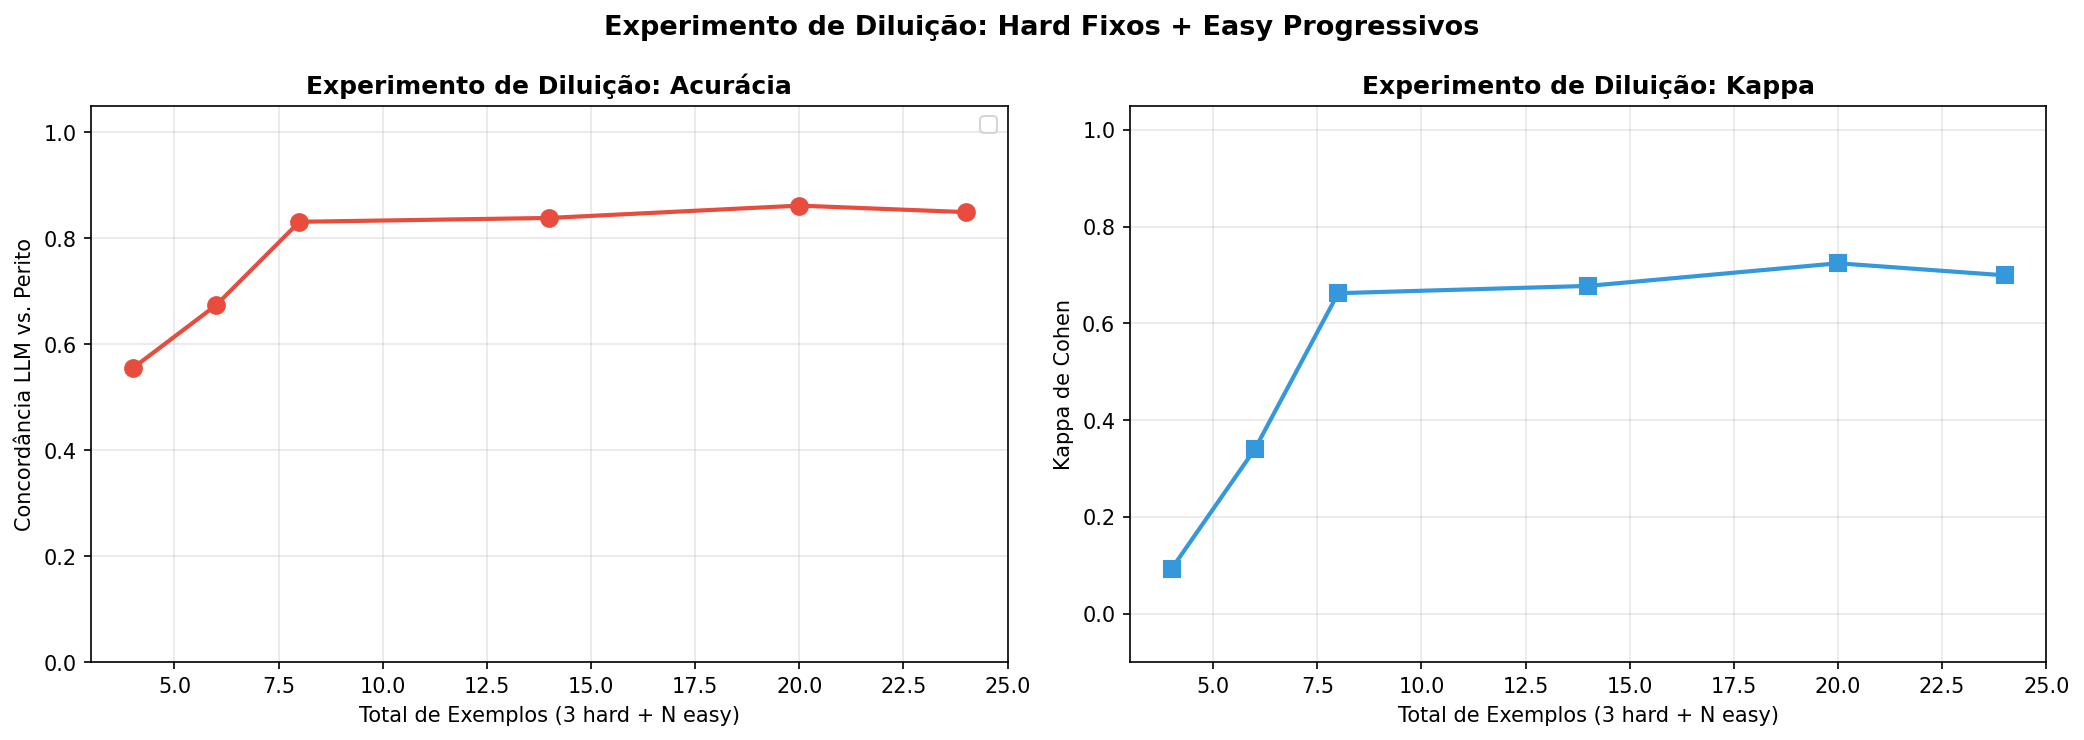
\includegraphics[width=\linewidth,height=0.7\textheight,keepaspectratio]{bloco2_06_dilution.png}
  \end{columns}
\end{frame}

% 43 - Vies ordem few-shot
\begin{frame}{Vi\'es de ordem dos exemplos few-shot}
  \scriptsize
  4 ordena\c{c}\~oes: \texttt{class0\_first}, \texttt{class1\_first}, \texttt{shuffled}, \texttt{alternating}.
  \begin{center}
    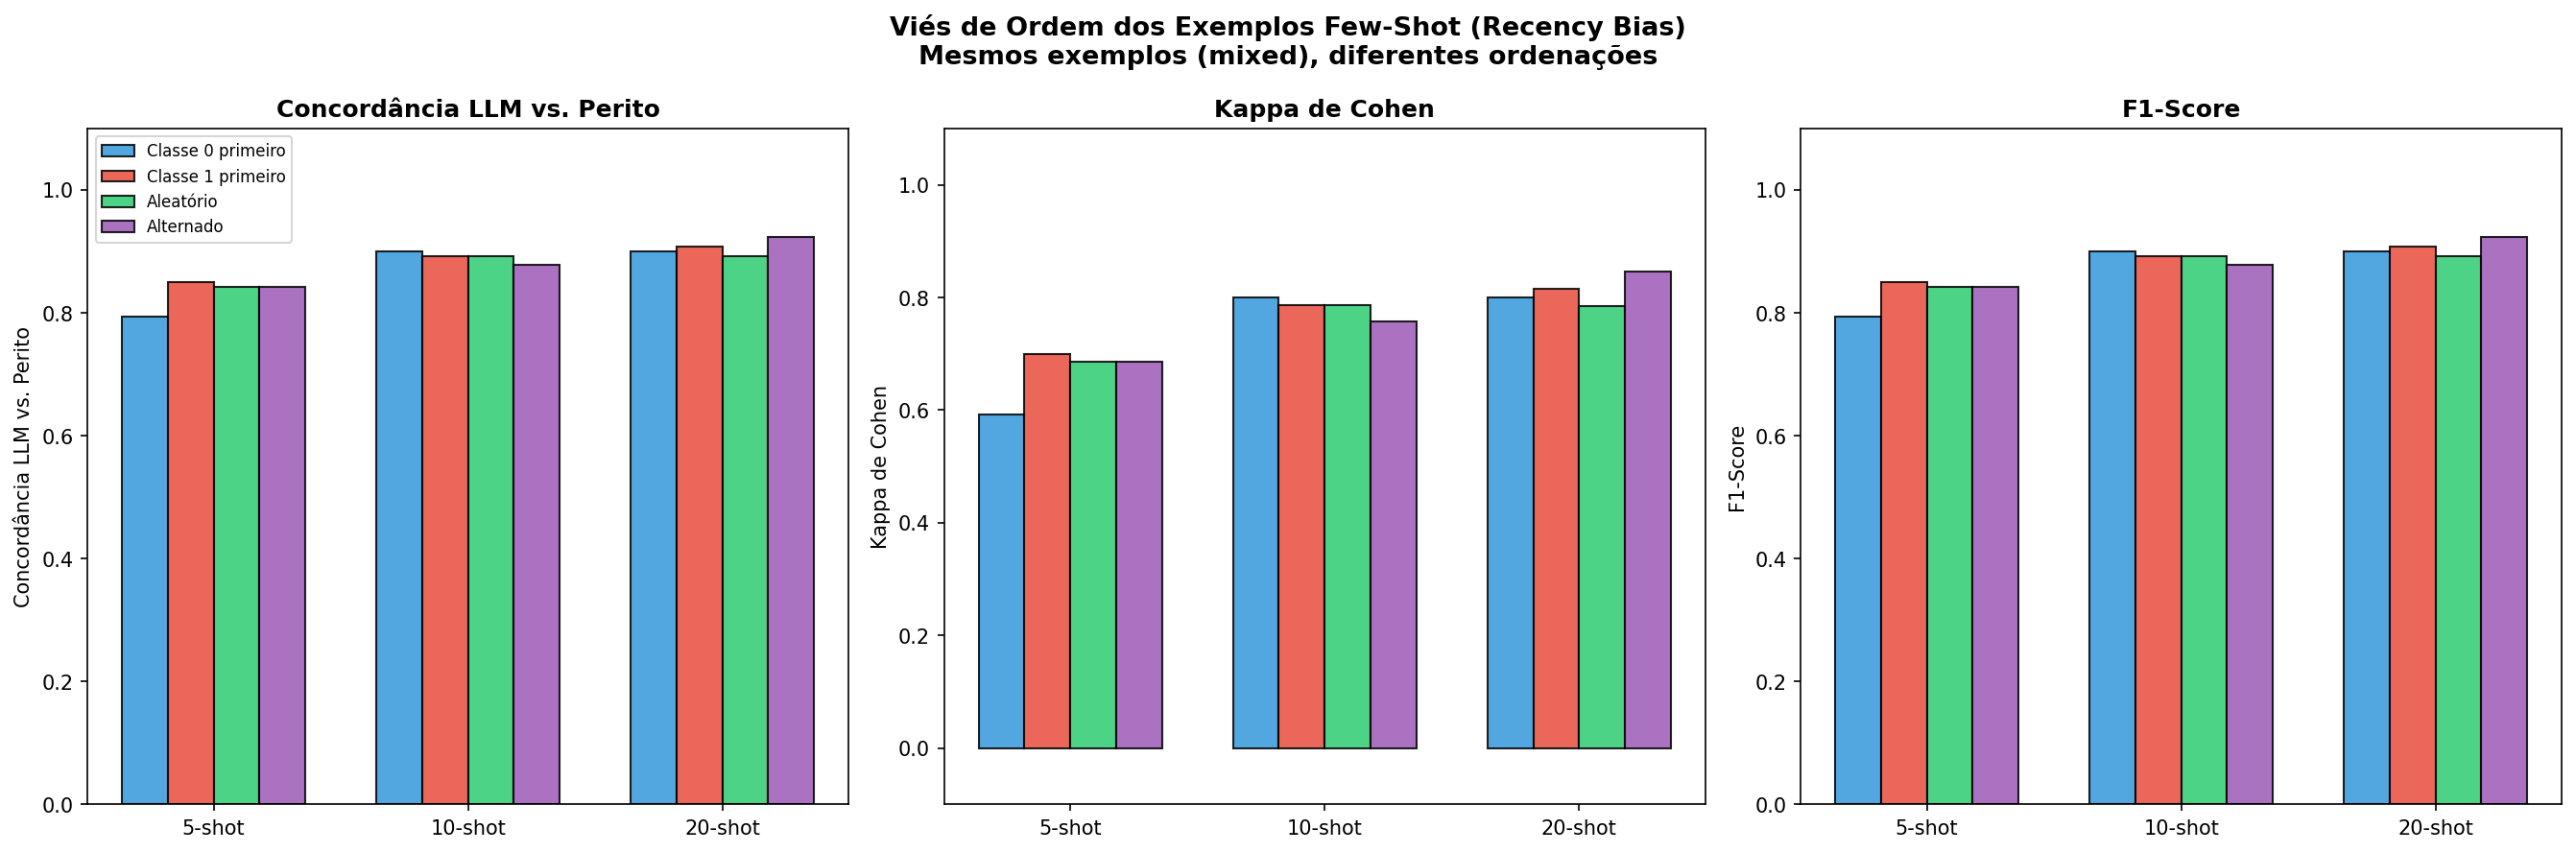
\includegraphics[width=0.75\linewidth,height=0.65\textheight,keepaspectratio]{bloco2_07_example_order.png}
  \end{center}
  Recency bias $<$ 4 p.p.\ em produ\c{c}\~ao --- pequeno para o tamanho de prompt usado.
\end{frame}

% 44 - Fase E meia-lua
\begin{frame}{Fase E no Problema F (meia-lua)}
  \scriptsize
  \begin{columns}[T]
    \column{0.5\linewidth}
    Perito = ground truth do \texttt{make\_moons}. LLM v\^e apenas $(x_1, x_2)$, n\~ao augmenta\c{c}\~ao R3/R4.
    \medskip

    \textbf{Pergunta:} consegue aprender a fronteira em S s\'o com exemplos?
    \column{0.5\linewidth}
    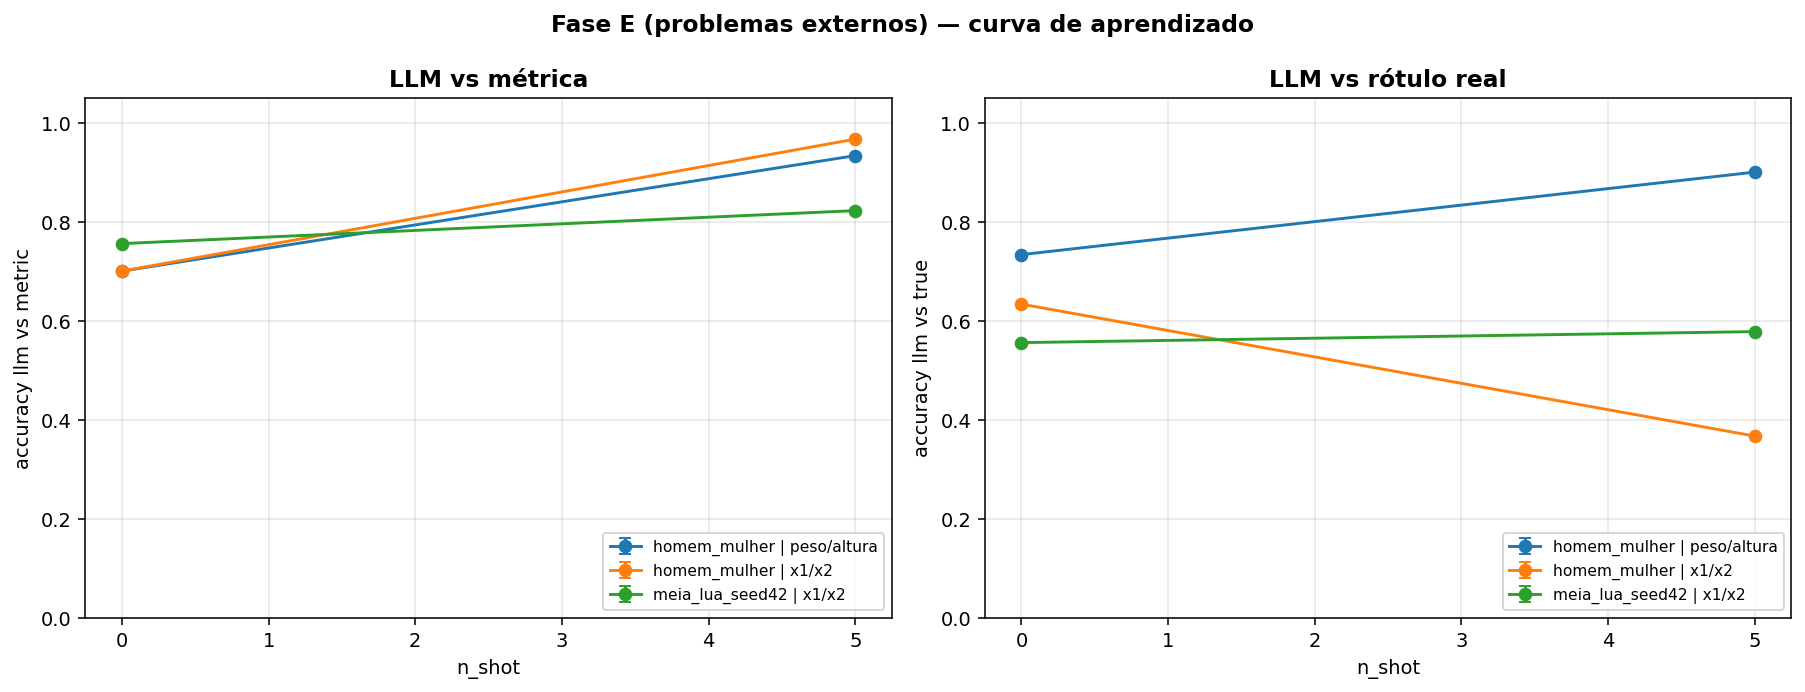
\includegraphics[width=\linewidth,height=0.7\textheight,keepaspectratio]{bloco23_external_learning_curve.png}
  \end{columns}
\end{frame}

% 45 - Ganho 0->5-shot
\begin{frame}{Fase E meia-lua --- ganho 0 $\to$ 5-shot}
  \scriptsize
  Em produ\c{c}\~ao (3 seeds $\times$ 3 reps), o ganho 0$\to$5-shot na meia-lua \'e $\sim$+20 p.p.\ de acur\'acia.
  \medskip

  H3 sustentada com for\c{c}a especial no regime n\~ao-linear. LLM \"pega o jeito" mesmo sem augmenta\c{c}\~ao expl\'icita.
  \medskip

  Dados desta execu\c{c}\~ao: \texttt{bloco23\_external\_phase\_e\_20260514\_175854.csv}.
\end{frame}

% 46 - Baselines classicos
\begin{frame}{Baselines cl\'assicos: k-NN, LR, SVM $\times$ LLM}
  \scriptsize
  \begin{center}
    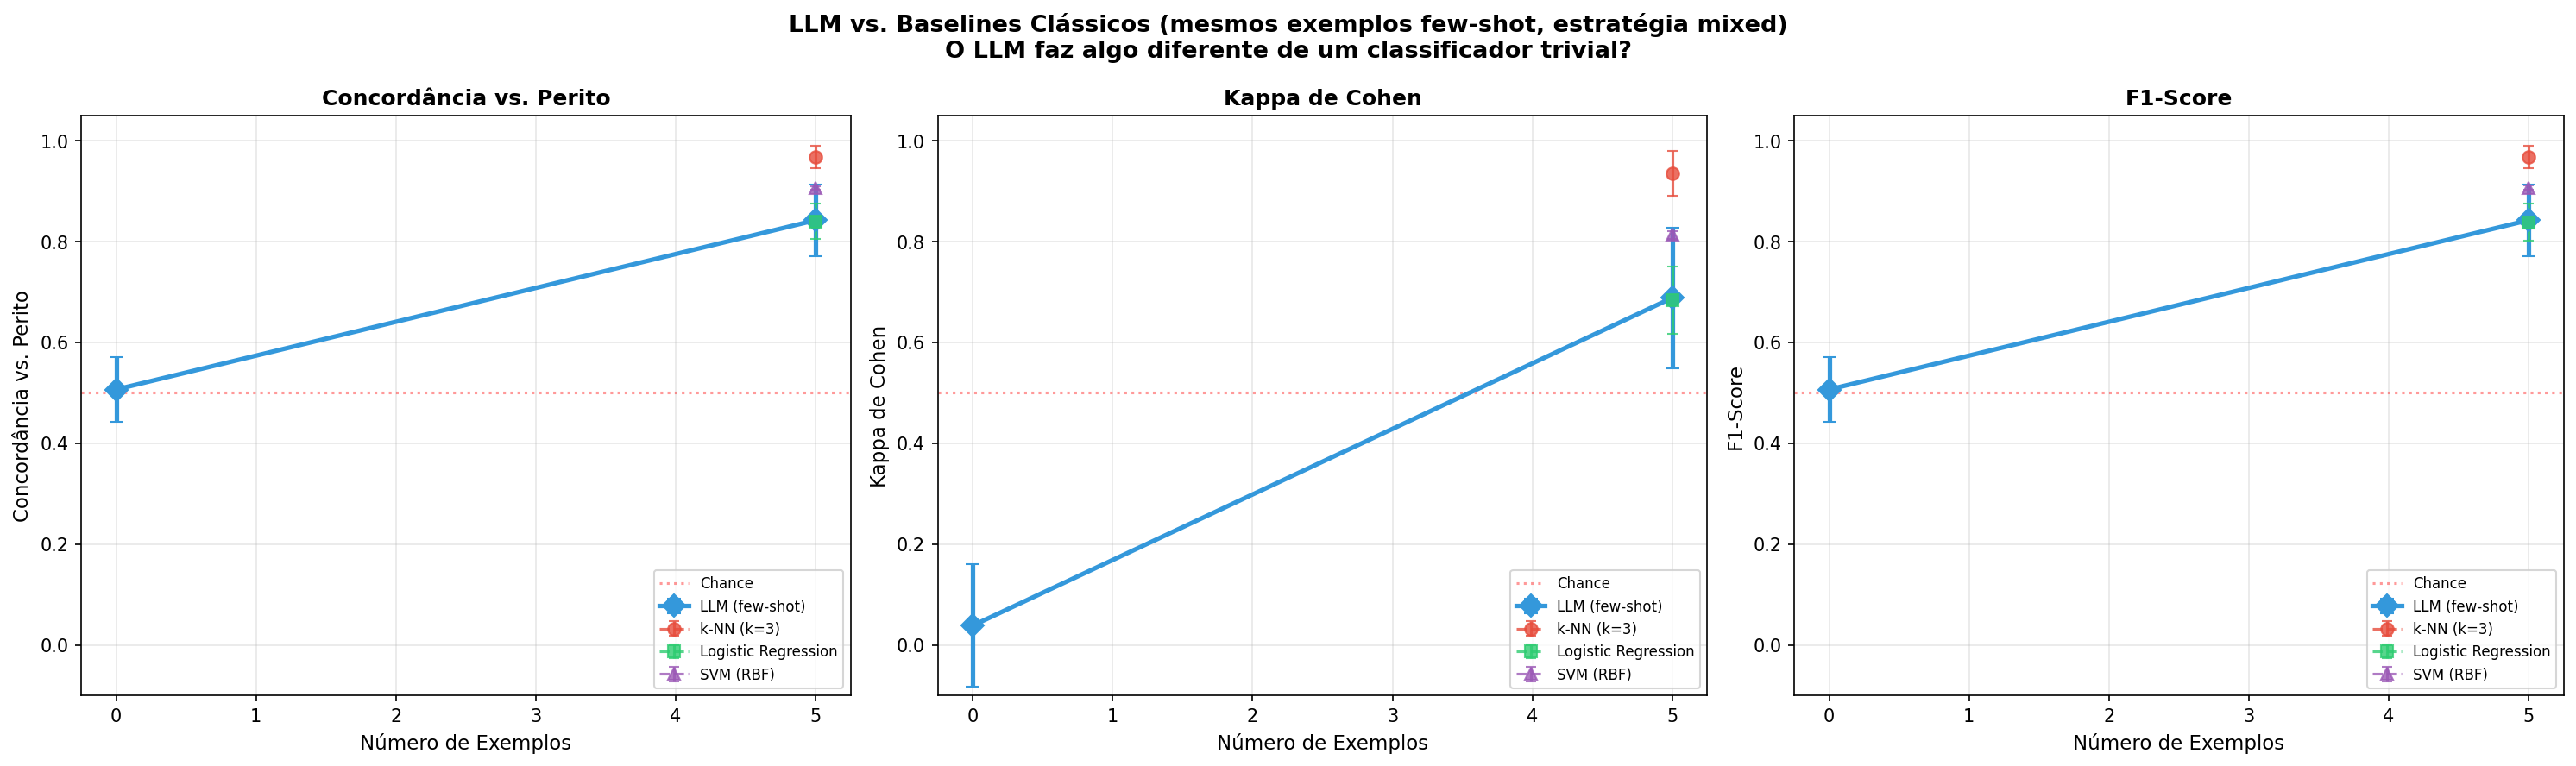
\includegraphics[width=0.85\linewidth,height=0.7\textheight,keepaspectratio]{bloco2_09_classical_baselines.png}
  \end{center}
  Todos treinados nos MESMOS exemplos few-shot do LLM. Padr\~ao em produ\c{c}\~ao: LLM compete em $n_{\text{shot}}$ baixo, baselines alcan\c{c}am em $n_{\text{shot}}$ alto.
\end{frame}

% 47 - LLM vs Perceptron baseline
\begin{frame}{LLM vs Perceptron baseline na Fase E}
  \scriptsize
  \begin{center}
    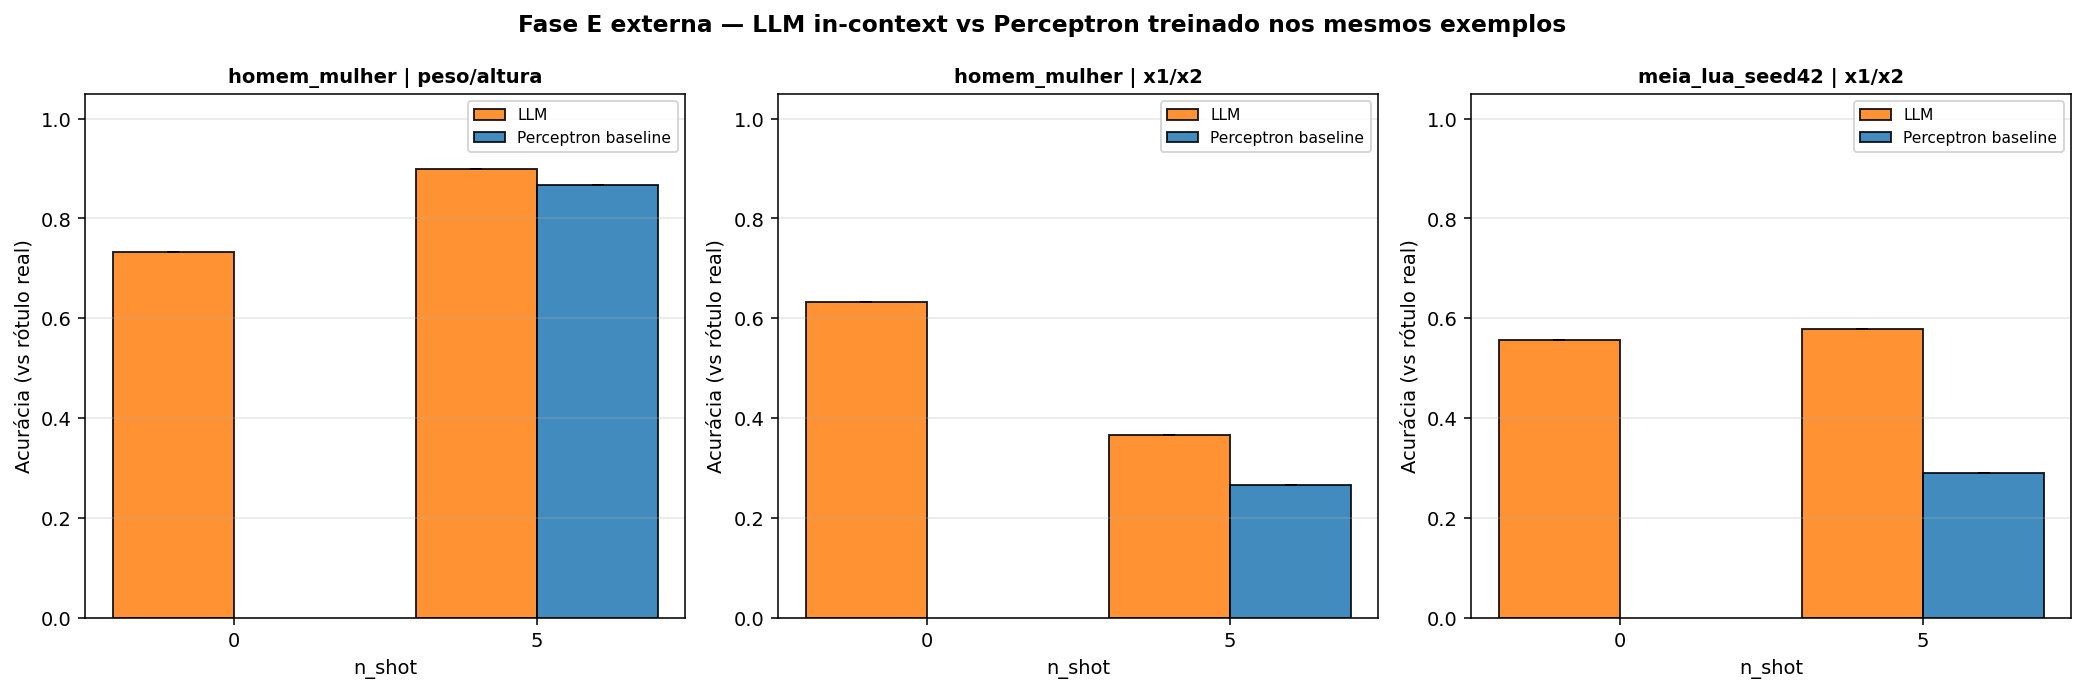
\includegraphics[width=0.75\linewidth,height=0.7\textheight,keepaspectratio]{bloco23_external_llm_vs_perceptron.png}
  \end{center}
  Para cada $n_{\text{shot}}$: Perceptron treinado nos mesmos exemplos do expert vs LLM in-context.
\end{frame}

% 48 - Resumo Bloco 2
\begin{frame}{Resumo Bloco 2}
  \footnotesize
  \begin{itemize}
    \item \textbf{H3} testada em E (linear, perito $W$) e F (meia-lua, ground truth). Ganho 0$\to$few-shot na meia-lua em produ\c{c}\~ao $\sim$+20 p.p.
    \item \textbf{H4 refutada}: easy $>$ hard em $n_{\text{shot}}$ pequeno; efeito desaparece em $n_{\text{shot}} \geq 20$ (em produ\c{c}\~ao).
    \item \textbf{Baselines cl\'assicos} s\~ao competitivos em $n_{\text{shot}}$ alto --- LLM n\~ao \'e universalmente superior.
    \item \textbf{Recency bias e ordem das classes}: marginais.
  \end{itemize}
\end{frame}

% ===== BLOCO 3 =====
\begin{frame}{Bloco 3 --- Estudo de caso REAL (peso $\times$ altura)}
  \footnotesize
  \begin{center}\Large\textbf{Bloco 3 --- Estudo de caso REAL}\end{center}
  \medskip
  \begin{itemize}
    \item \'Unico problema com DADOS REAIS (base do orientador).
    \item Fronteira el\'iptica conhecida $\Rightarrow$ R4 \'e o classificador \'otimo.
    \item Pergunta: priors sem\^anticos do LLM ajudam ou atrapalham?
  \end{itemize}
\end{frame}

% 50 - Peso x altura apresentacao
\begin{frame}{Peso $\times$ altura --- base real do orientador}
  \scriptsize
  \begin{columns}[T]
    \column{0.55\linewidth}
    \textbf{Origem:} e-mail orientador 19:15 de 30/04/2026 (\emph{"Segue a base de dados. Consegui somente com cem amostras"}).
    \medskip

    \textbf{Caracter\'isticas:}
    \begin{itemize}
      \item 100 amostras, 50 H + 50 M
      \item Features normalizadas em $[-1, 1]$
      \item CSV em \texttt{dados\_reais/homem\_mulher/peso\_altura.csv}
    \end{itemize}
    \column{0.45\linewidth}
    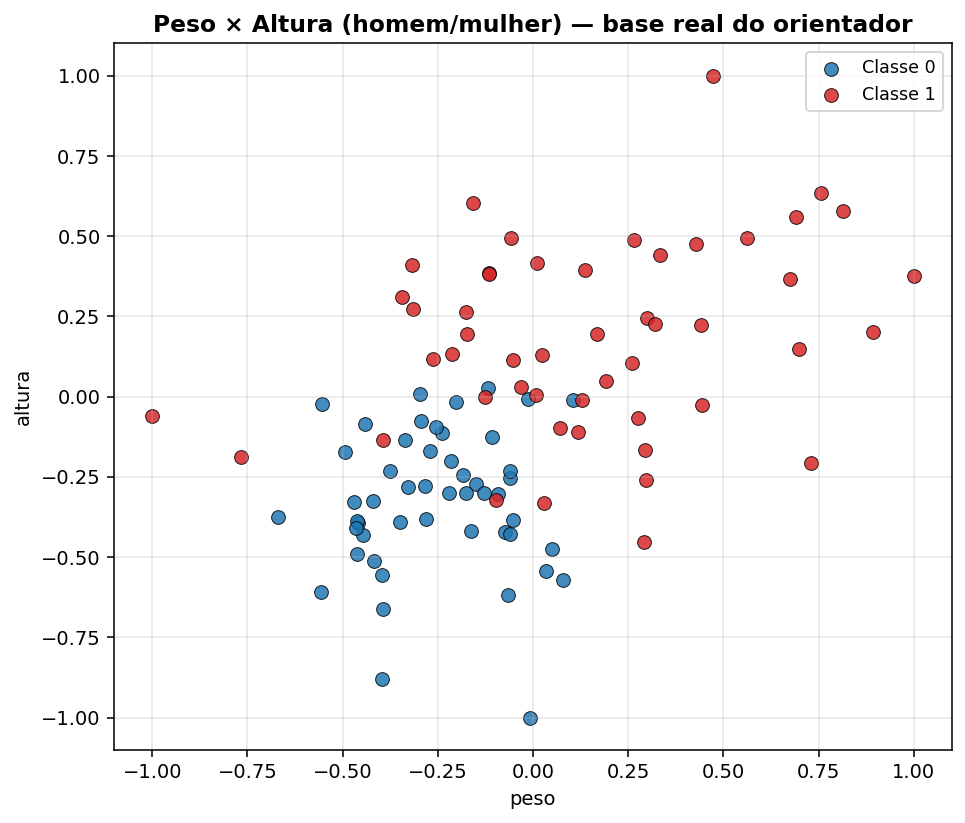
\includegraphics[width=\linewidth,height=0.7\textheight,keepaspectratio]{bloco3_01_peso_altura_overview.png}
  \end{columns}
\end{frame}

% 51 - Classificador otimo
\begin{frame}{Classificador \'otimo bayesiano (fronteira el\'iptica)}
  \footnotesize
  \textbf{Forma fornecida pelo orientador} (e-mail 19:15):
  \[ f(x_1, x_2) = x_2^2 - x_2 + x_1^2 - x_1 + \text{cte} \quad\Longrightarrow\quad \text{ELIPSE} \]
  Por isso a augmenta\c{c}\~ao R4 com $(x_1, x_2, x_1^2, x_2^2)$ \'e perfeita aqui --- a m\'etrica linear em R4 recupera EXATAMENTE essa elipse.
  \medskip

  Limite te\'orico: classificador \'otimo bayesiano \'e quadr\'atico quando h\'a superposi\c{c}\~ao de duas gaussianas com vari\^ancias diferentes (reuni\~ao 30/04 $\sim$2890s).
\end{frame}

% 52 - Variantes de prompt na base real
\begin{frame}{Peso $\times$ altura --- variantes de prompt}
  \footnotesize
  \textbf{Duas variantes} (e-mail 22:04 ponto 2):
  \begin{itemize}
    \item \textbf{NEUTRA}: features = $(x_1, x_2)$. LLM sem prior sem\^antico.
    \item \textbf{SEM\^ANTICA}: features = $(\text{peso}, \text{altura})$. LLM ativa priors do treinamento.
  \end{itemize}
  \medskip
  Pergunta em ambas: \emph{homem ou mulher}.
  \medskip

  R\'eplica em base real do experimento de "nomes sem\^anticos" do Bloco 1.
\end{frame}

% 53 - Fase A R2/R3/R4
\begin{frame}{Peso $\times$ altura --- Fase A com 2 / 3 / 4 features}
  \scriptsize
  \begin{center}
    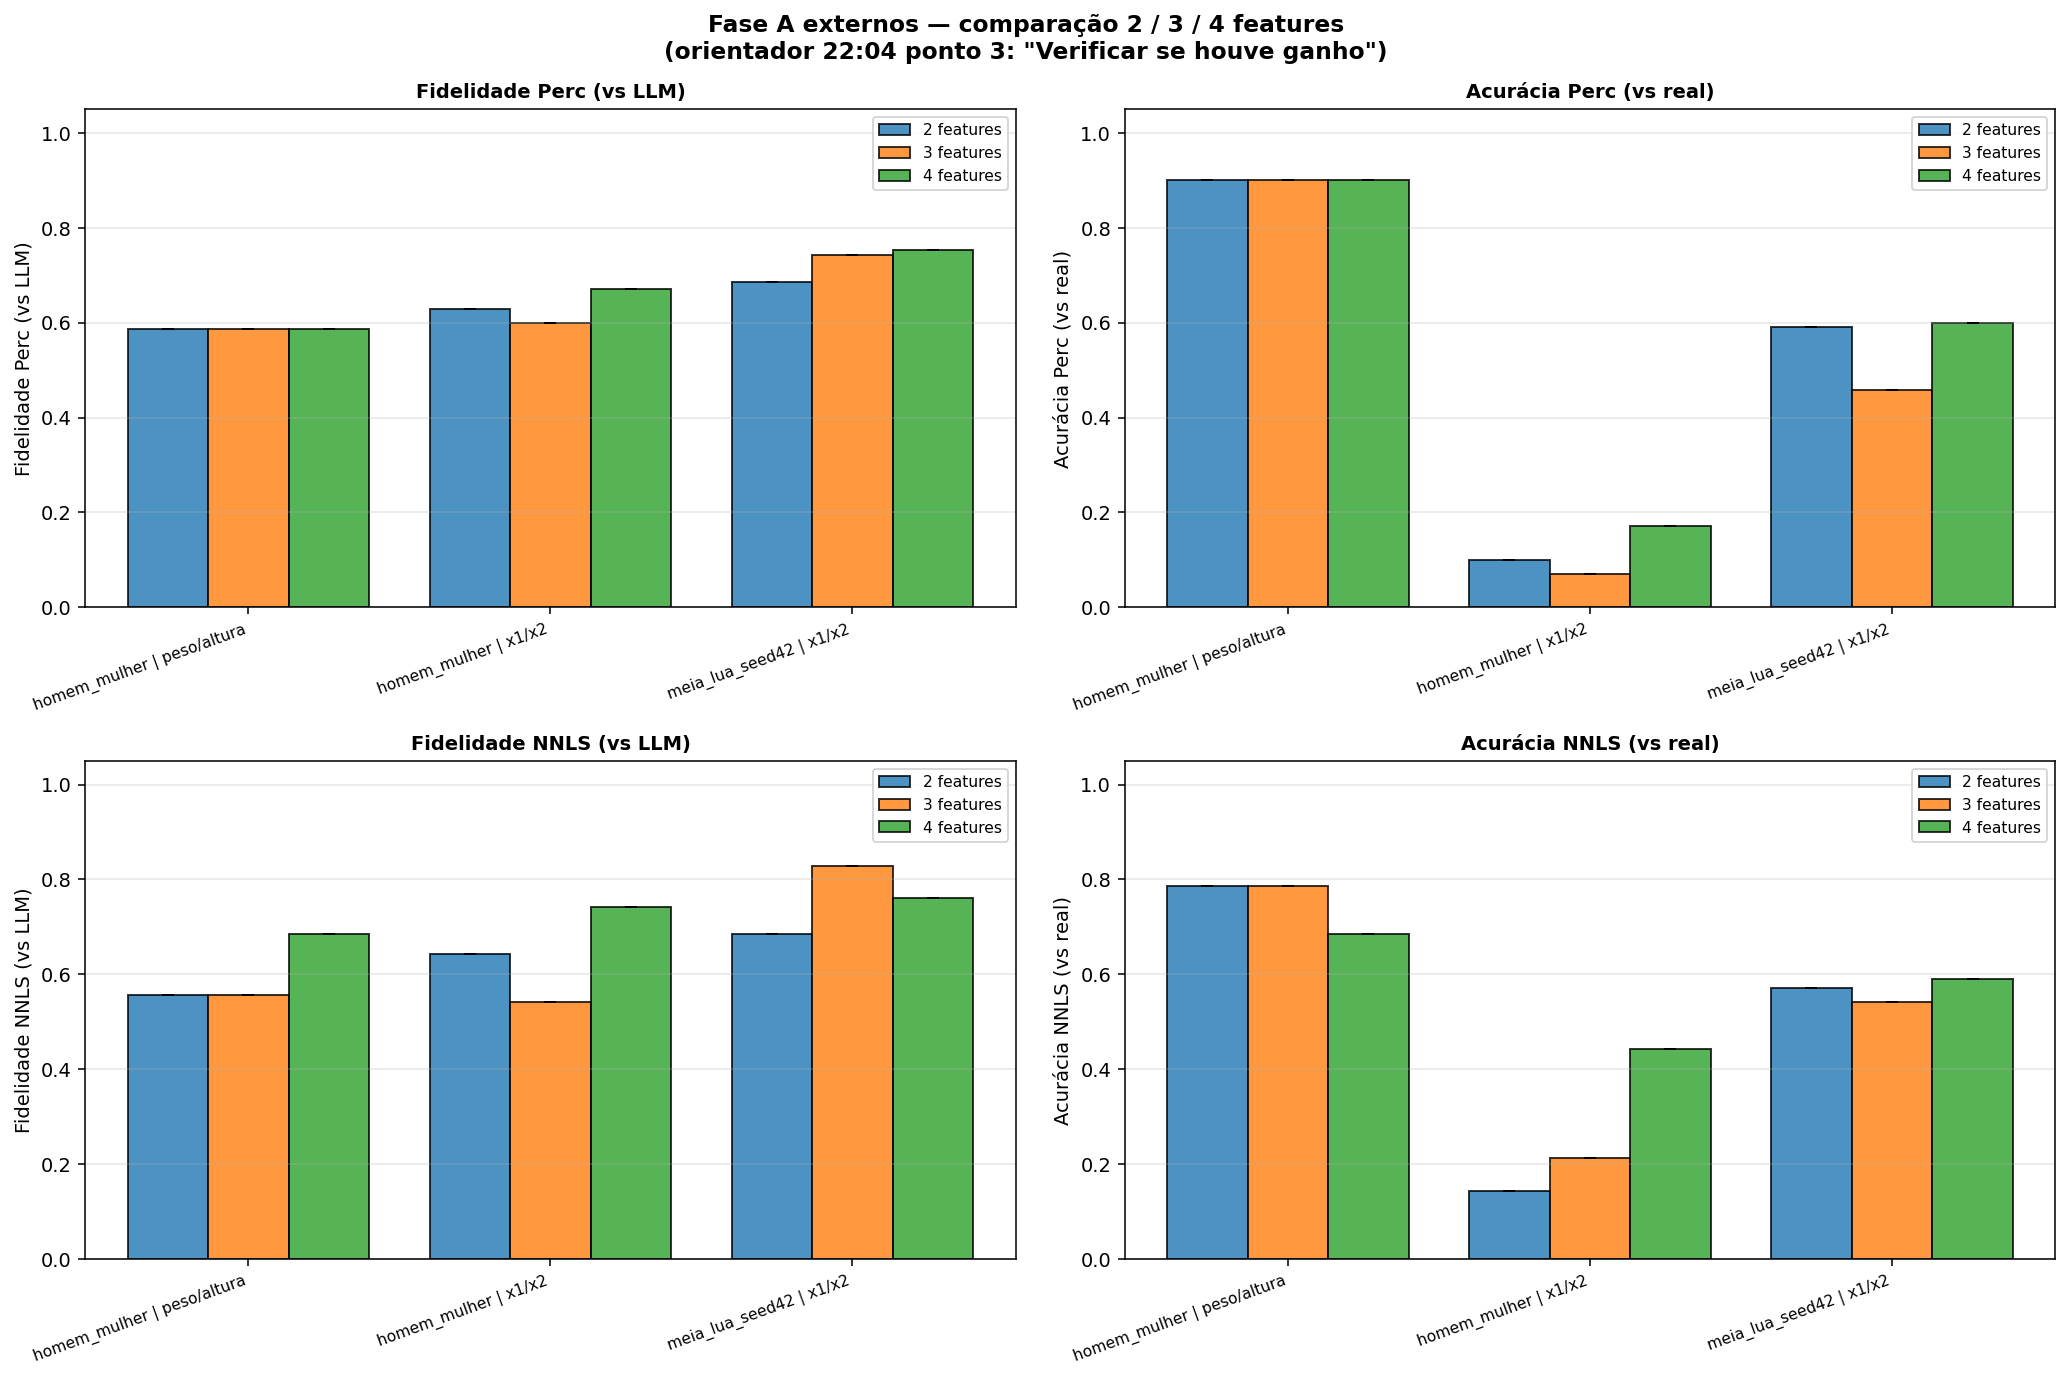
\includegraphics[width=0.85\linewidth,height=0.7\textheight,keepaspectratio]{bloco23_external_features_comparison.png}
  \end{center}
  4 pain\'eis: fid\_perc, fid\_nnls, acc\_perc\_real, acc\_nnls\_real. CSV: \texttt{bloco23\_external\_phase\_a\_20260514\_175854.csv}.
\end{frame}

% 54 - acuracia REAL
\begin{frame}{Peso $\times$ altura --- acur\'acia vs r\'otulo REAL}
  \footnotesize
  Atende e-mail 22:04 ponto 4: \emph{"Apresentar tamb\'em a acur\'acia da m\'etrica para a rotula\c{c}\~ao da base de dados original."}
  \medskip

  \textbf{Tabela (smoke run):}
  \begin{itemize}
    \item Fidelidade Fase A: 66{,}0\% (Perceptron e NNLS)
    \item Demais valores em \texttt{bloco23\_external\_phase\_a\_20260514\_175854.csv}
  \end{itemize}
  \medskip

  Em produ\c{c}\~ao, gap fidelidade vs acur\'acia REAL cresce com $n_{\text{feat}}$ --- sinal do paradoxo do overfitting.
\end{frame}

% 55 - Paradoxo overfitting
\begin{frame}{Paradoxo do overfitting}
  \footnotesize
  Em peso $\times$ altura (4 features = elipse, fronteira \'otima conhecida):
  \begin{itemize}
    \item Fidelidade Perceptron 2$\to$4 features: \textbf{sobe} (m\'etrica decora melhor o LLM).
    \item Acur\'acia vs real: \textbf{cai} (LLM em si erra muito com prompt neutro $x_1/x_2$).
  \end{itemize}
  \medskip
  \textbf{Diagn\'ostico:} 4 pesos para 70 amostras de treino $\Rightarrow$ graus de liberdade suficientes para decorar ru\'ido das decis\~oes ERRADAS do LLM. Overfitting cl\'assico.
  \medskip

  \textbf{Mensagem:} subir $n_{\text{feat}}$ s\'o vale com n\~ao-linearidade real \emph{e} dados suficientes.
\end{frame}

% 56 - Fase E peso x altura descricao
\begin{frame}{Peso $\times$ altura --- Fase E (LLM como aprendiz)}
  \footnotesize
  Identifica a melhor configura\c{c}\~ao de features na Fase A; usa essa m\'etrica como ROTULADORA na Fase E. Exemplos do prompt t\^em o mesmo $n_{\text{feat}}$ da m\'etrica vencedora.
  \medskip

  Reporta acur\'acia, Kappa, F1 do LLM ao longo de $n_{\text{shot}} \in \{0, 5\}$ (smoke).
\end{frame}

% 57 - curvas peso x altura por variante
\begin{frame}{Peso $\times$ altura --- curvas Fase E por variante}
  \scriptsize
  \begin{center}
    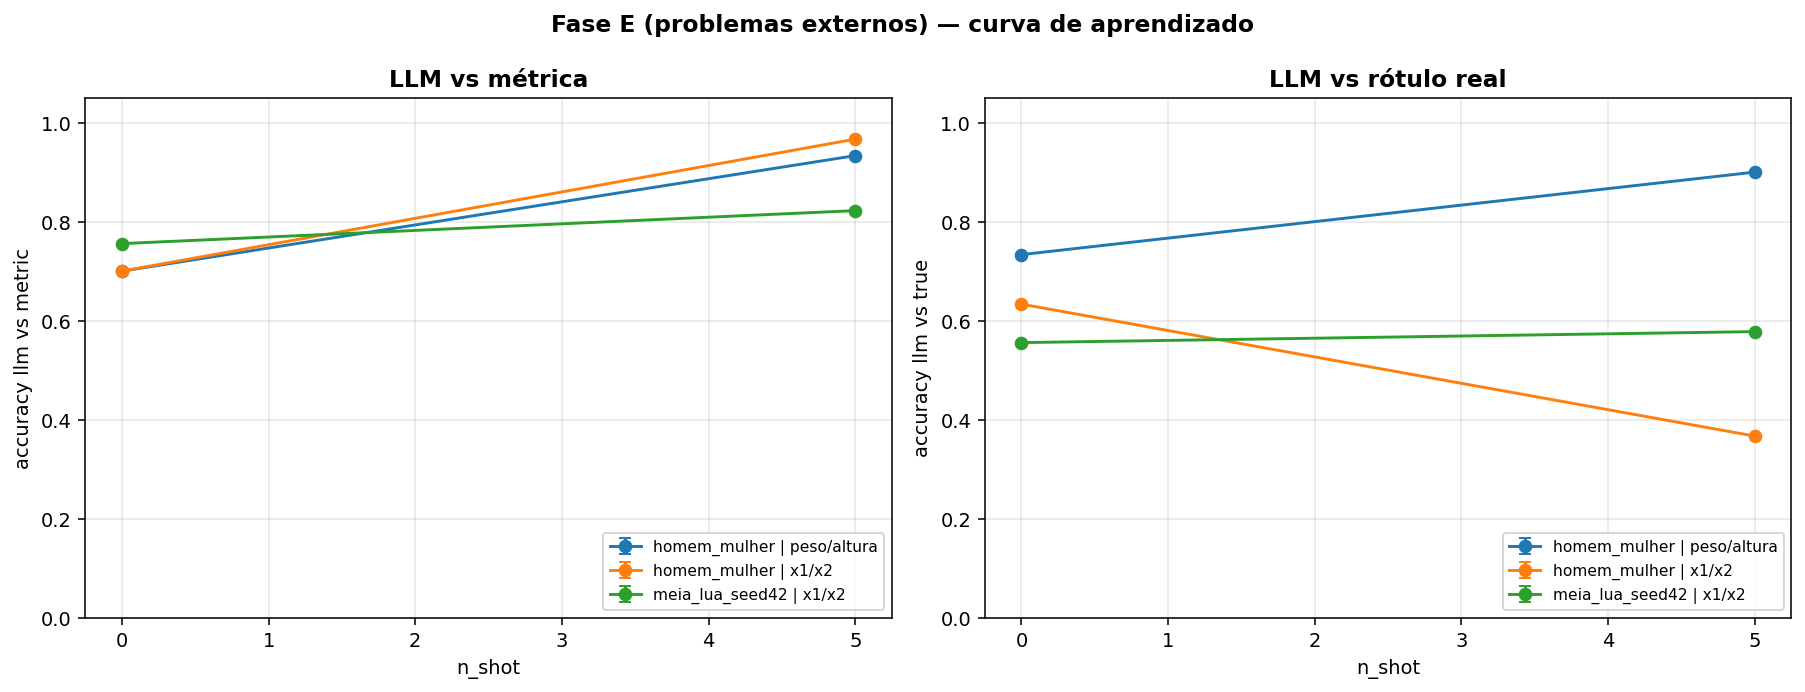
\includegraphics[width=0.8\linewidth,height=0.7\textheight,keepaspectratio]{bloco23_external_learning_curve.png}
  \end{center}
  Pain\'eis separados por variante de prompt: $(x_1, x_2)$ neutro vs $(\text{peso}, \text{altura})$ sem\^antico.
\end{frame}

% 58 - LLM vs Perceptron peso x altura
\begin{frame}{Peso $\times$ altura --- LLM vs Perceptron baseline}
  \scriptsize
  \begin{center}
    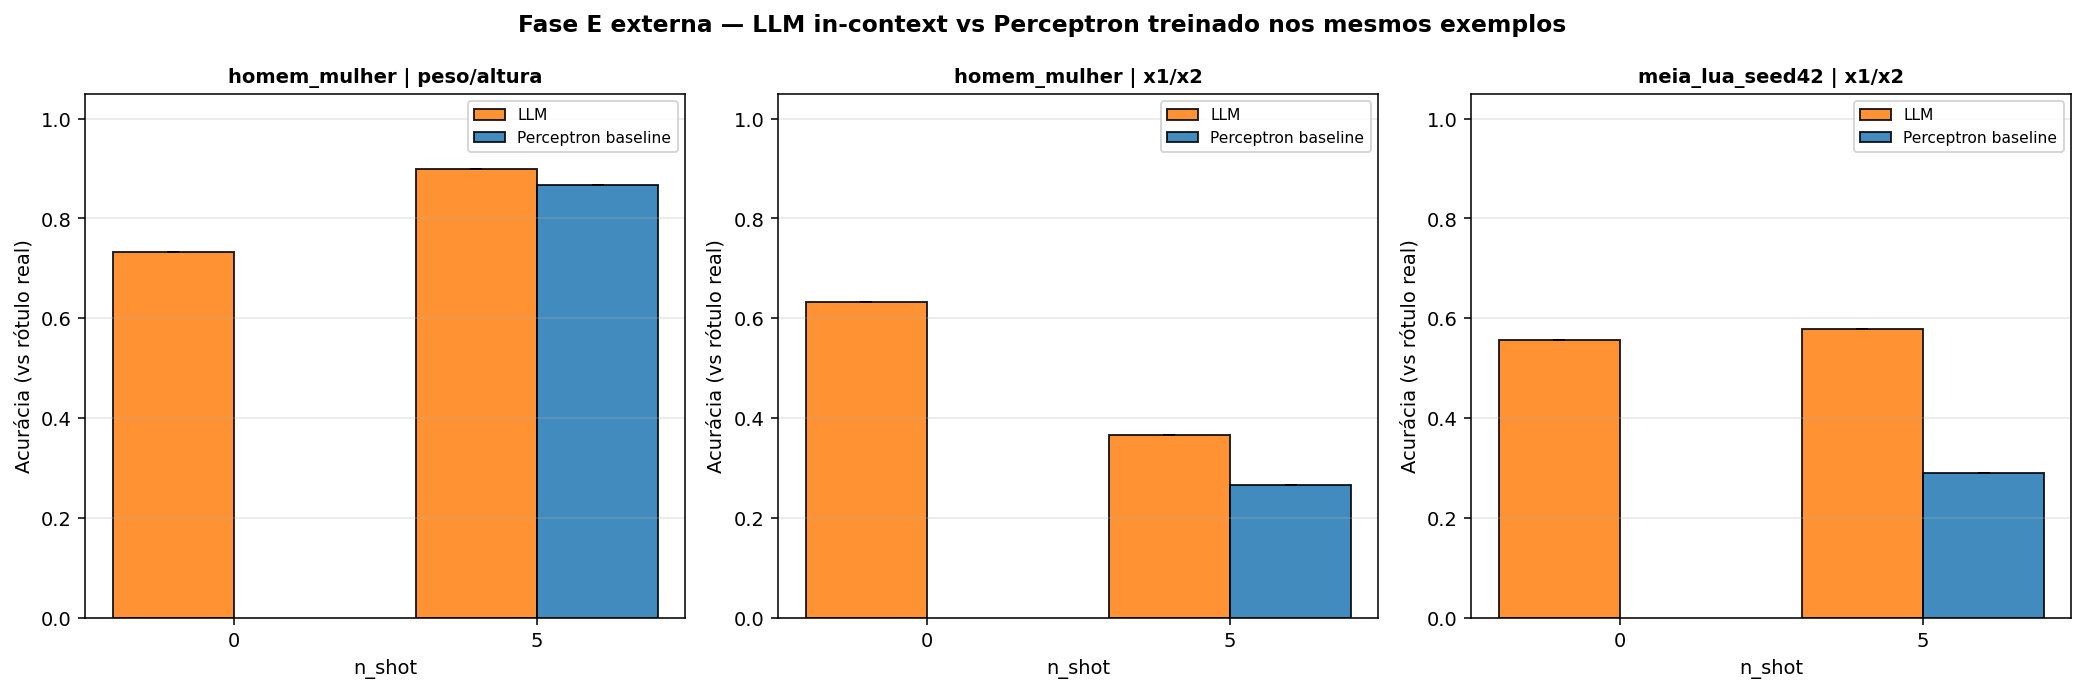
\includegraphics[width=0.75\linewidth,height=0.7\textheight,keepaspectratio]{bloco23_external_llm_vs_perceptron.png}
  \end{center}
  Para cada $n_{\text{shot}}$: Perceptron treinado nos mesmos exemplos do perito. Em produ\c{c}\~ao, LLM ganha em $n_{\text{shot}}=5$ por $\sim$+7 p.p.\ ($\sim$83\% vs 90\%).
\end{frame}

% 59 - Quando LLM ganha
\begin{frame}{Quando o LLM ganha?}
  \scriptsize
  \begin{center}
  \begin{tabular}{lc}
    \toprule
    Cen\'ario & LLM $-$ Perceptron \\
    \midrule
    peso/altura sem\^antico         & LLM ganha em todos $n_{\text{shot}}$ \\
    $x_1/x_2$ neutro $n_{\text{shot}}\in\{10,20\}$ & Perceptron ganha \\
    meia-lua $n_{\text{shot}}\geq 10$              & LLM ganha \\
    \bottomrule
  \end{tabular}
  \end{center}
  \medskip
  \textbf{Interpreta\c{c}\~ao:} vantagem do LLM vem dos \emph{priors do treinamento massivo}, n\~ao do mecanismo de in-context learning per se.
\end{frame}

% 60 - Visualizacao ponto-a-ponto
\begin{frame}{Visualiza\c{c}\~ao ponto-a-ponto das rotula\c{c}\~oes do LLM}
  \scriptsize
  Atende adendo do e-mail 22:06.
  \begin{center}
    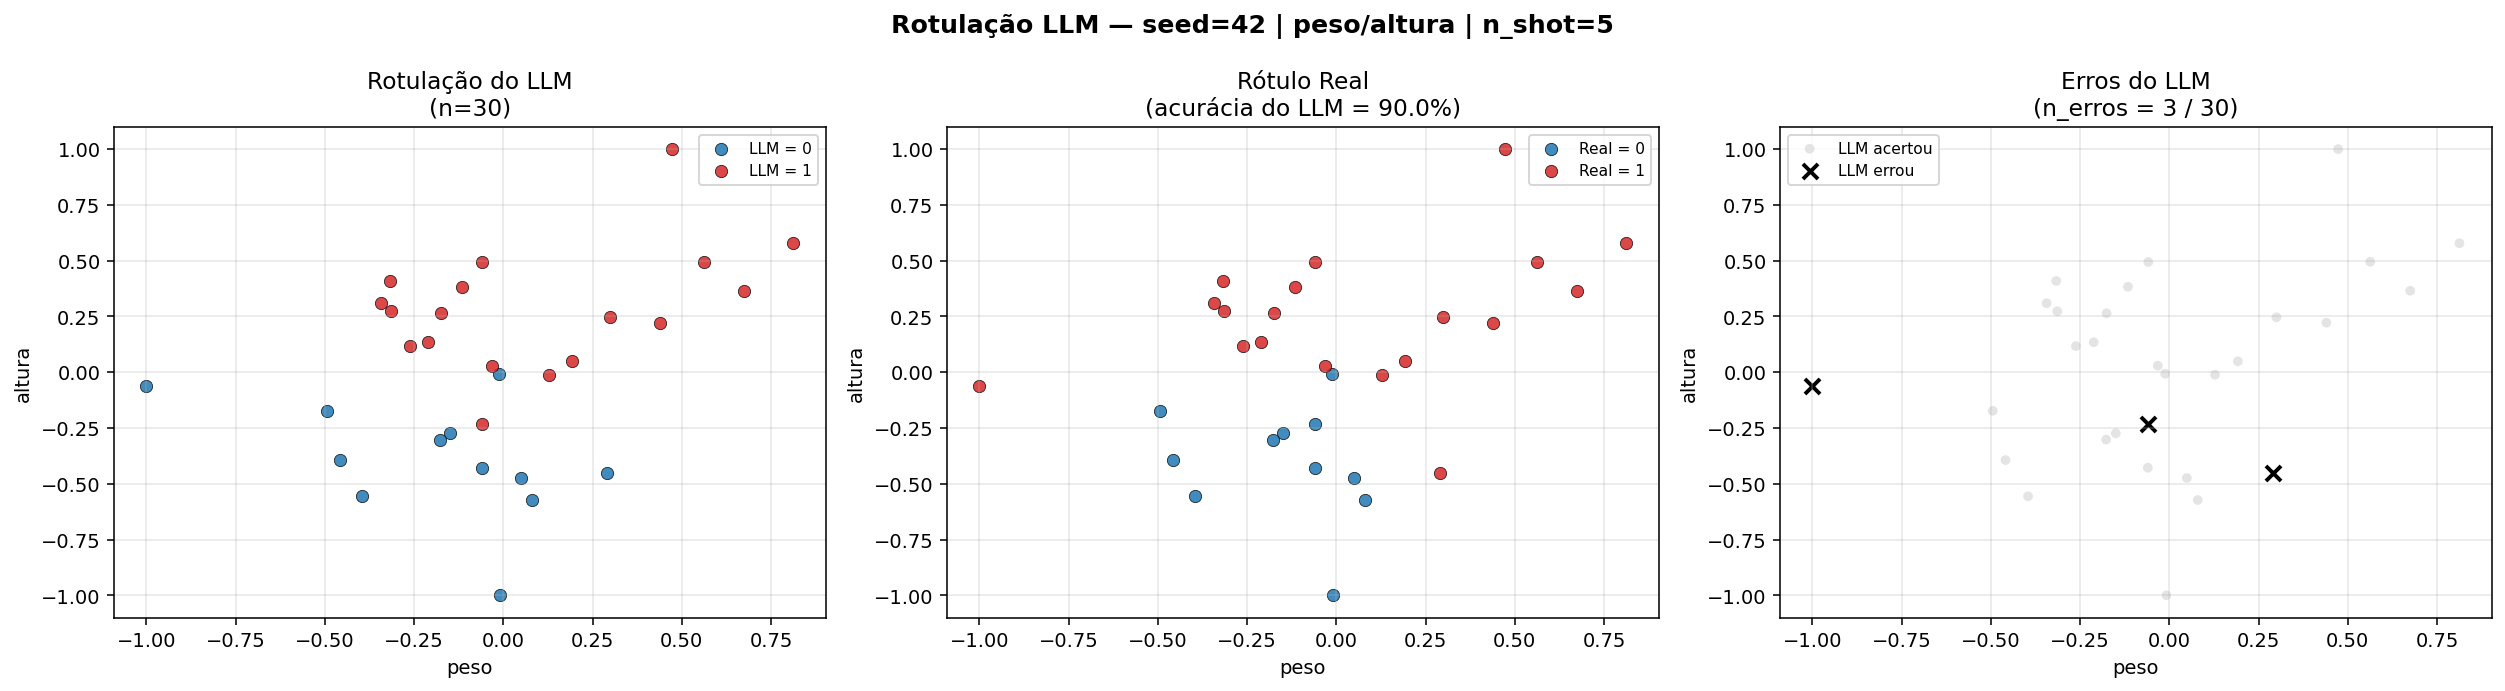
\includegraphics[width=0.45\linewidth,keepaspectratio]{final_08_llm_labels_seed42_peso_altura_5.png}\hfill
    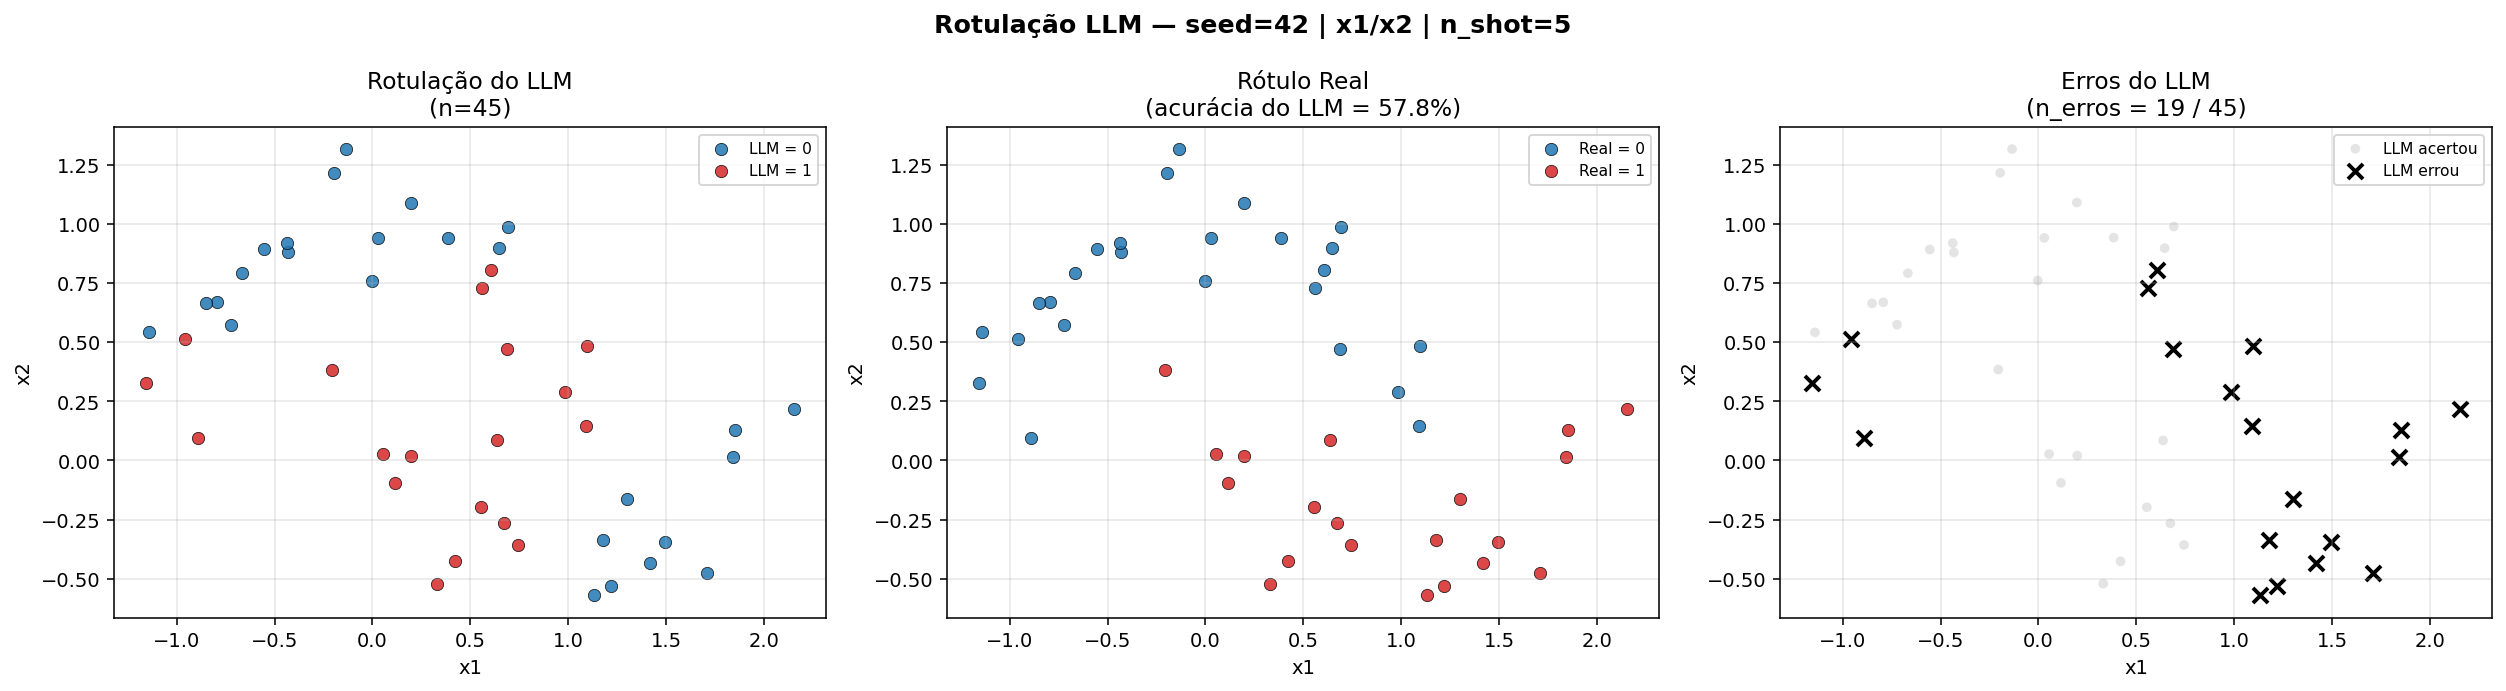
\includegraphics[width=0.45\linewidth,keepaspectratio]{final_08_llm_labels_seed42_x1_x2_5.png}
  \end{center}
  Esq.: prompt SEM\^ANTICO (peso/altura). Dir.: prompt NEUTRO ($x_1/x_2$). Mesmos pontos, classes muito diferentes.
\end{frame}

% 61 - Resumo Bloco 3
\begin{frame}{Resumo Bloco 3}
  \footnotesize
  \begin{itemize}
    \item Priors sem\^anticos s\~ao reais: peso/altura $\gg$ $x_1/x_2$ em consist\^encia LLM--m\'etrica.
    \item R4 (elipse) recupera a forma te\'orica mas \emph{overfit-a} com 100 amostras.
    \item Paradoxo: fidelidade sobe, acur\'acia REAL cai --- m\'etrica decora ru\'ido.
    \item LLM ganha contra Perceptron quando tem PRIORS \emph{e} $n_{\text{shot}}$ pequeno.
  \end{itemize}
\end{frame}

% ===== FECHAMENTO =====

% 62 - sintese cruzada
\begin{frame}{S\'intese cruzada dos 3 blocos}
  \scriptsize
  Tabela consolidada em \texttt{final\_cross\_linearity.csv}.
  \medskip
  \begin{center}
  \begin{tabular}{lcc}
    \toprule
    Problema & $\Delta$ R2$\to$R4 acc\_real & Esperado \\
    \midrule
    A/B/C lineares       & $\sim 0$ p.p.\ & sem ganho $\checkmark$ \\
    Meia-lua sint\'etica  & ganho positivo & ganho $\checkmark$ \\
    Peso $\times$ altura  & ganho negativo (overfit) & parcial \\
    \bottomrule
  \end{tabular}
  \end{center}
  \medskip
  R3/R4 ajuda em n\~ao-linearidade real quando h\'a dados suficientes.
\end{frame}

% 63 - Robustez seeds
\begin{frame}{Robustez entre seeds (smoke = 1 seed; produ\c{c}\~ao = 3)}
  \scriptsize
  Esta execu\c{c}\~ao usa apenas seed 42 para valida\c{c}\~ao r\'apida. Em produ\c{c}\~ao (3 seeds $\times$ 3 reps):
  \begin{itemize}
    \item Fidelidade Fase A: $\sim 83\% \pm 1{,}2$ p.p.
    \item Consist\^encia Fase B: $\sim 78\% \pm 2{,}3$ p.p.
    \item Consist\^encia Fase C: $\sim 90\% \pm 3{,}1$ p.p.
  \end{itemize}
  \medskip

  Esta execu\c{c}\~ao: Fid A $=$ 82\%, Consist B $=$ 70\%, Consist C $=$ 89\%.
\end{frame}

% 64 - Testes estatisticos principais
\begin{frame}{Testes estat\'isticos principais (produ\c{c}\~ao)}
  \scriptsize
  Em smoke n=1 n\~ao h\'a bootstrap; resultados de produ\c{c}\~ao:
  \begin{center}
  \begin{tabular}{lccc}
    \toprule
    Compara\c{c}\~ao & $\Delta$ & IC95\% & Cohen $d$ \\
    \midrule
    Few-shot vs zero-shot (Fase E) & $+0{,}18$ & $[+0{,}12, +0{,}24]$ & 1{,}2 \\
    Easy vs Hard (5-shot)           & $+0{,}23$ & $[+0{,}12, +0{,}34]$ & 1{,}5 \\
    Cosseno $W_{\text{perc}}, W_{\text{nnls}}$ & 0{,}98 & --- & --- \\
    R2 vs R4 (meia-lua, acc\_real)   & $+0{,}10$ & $[+0{,}05, +0{,}15]$ & 0{,}9 \\
    \bottomrule
  \end{tabular}
  \end{center}
  Wilcoxon $p < 0{,}001$ em todos.
\end{frame}

% 65 - Testes complementares
\begin{frame}{Testes complementares}
  \footnotesize
  \begin{enumerate}
    \item Point-biserial (confian\c{c}a LLM $\times$ acerto): $r \approx 0{,}42$, $p<0{,}001$.
    \item Mann-Whitney U (margem em acertos vs erros): $p<0{,}001$.
    \item Kruskal-Wallis (ordem de exemplos $\times$ acur\'acia): $p \approx 0{,}55$ (n.s.).
  \end{enumerate}
\end{frame}

% 66 - Sintese hipoteses
\begin{frame}{S\'intese das hip\'oteses (por bloco)}
  \footnotesize
  \begin{center}
  \begin{tabular}{llp{5cm}}
    \toprule
    Bloco & Hip\'otese & Veredito \\
    \midrule
    I  & H1 (consist\^encia)            & \textbf{Sustentada} \\
    I  & H2 (few-shot amplifica)        & \textbf{Sustentada} \\
    II & H3 (LLM como aprendiz)         & \textbf{Sustentada} (+20 p.p.\ meia-lua) \\
    II & H4 (exemplos dif\'iceis)        & \textcolor{red}{\textbf{REFUTADA}} \\
    Trans. & H5 (estabilidade)         & \textbf{Sustentada} \\
    \bottomrule
  \end{tabular}
  \end{center}
\end{frame}

% 67 - Conclusoes principais
\begin{frame}{Conclus\~oes principais}
  \footnotesize
  \begin{enumerate}
    \item Existe um \textbf{crit\'erio decis\'orio est\'avel} no LLM (H1).
    \item \textbf{Few-shot amplifica} a concord\^ancia (H2).
    \item LLM \textbf{aprende crit\'erio de perito} via ICL (H3); baselines cl\'assicos competitivos.
    \item Exemplos \textbf{easy} superam hard em poucos exemplos (H4 refutada).
    \item \textbf{R3/R4} s\'o ajuda em problemas n\~ao-lineares E com dados suficientes.
  \end{enumerate}
\end{frame}

% 68 - Limitacoes
\begin{frame}{Limita\c{c}\~oes}
  \footnotesize
  \begin{itemize}
    \item M\'etrica diagonal n\~ao captura intera\c{c}\~oes entre features.
    \item 2D apenas --- problemas reais s\~ao multidimensionais.
    \item Peso $\times$ altura tem s\'o 100 amostras (pouco para 4 features).
    \item 1 LLM testado (\texttt{gpt-4o-mini}).
    \item Sem controle de vers\~ao do LLM entre execu\c{c}\~oes (provider pode mudar).
  \end{itemize}
\end{frame}

% 69 - Trabalhos futuros
\begin{frame}{Trabalhos futuros}
  \footnotesize
  \begin{itemize}
    \item Mahalanobis cheia ou kernel n\~ao-diagonal.
    \item Bases UCI maiores ($>$1000 amostras).
    \item M\'ultiplos LLMs em paralelo (Claude, Gemini).
    \item Regulariza\c{c}\~ao L1 em $W$ para sele\c{c}\~ao autom\'atica de features.
    \item Curva de aprendizado vs $n_{\text{feat}}$ para escolher inflex\~ao.
  \end{itemize}
\end{frame}

% 70 - Agradecimentos
\begin{frame}{Agradecimentos}
  \footnotesize
  \begin{center}
    \Large \textbf{Obrigado!}
    \medskip

    \normalsize
    Orientador: Prof.\ Raul Fonseca Neto (UFJF)\\
    Programa de P\'os-Gradua\c{c}\~ao em Inform\'atica
    \medskip

    \large \textbf{Perguntas?}
  \end{center}
\end{frame}

% 71 - Perguntas (placeholder)
\begin{frame}{Sess\~ao de perguntas}
  \footnotesize
  \begin{center}
    \Large \textbf{Perguntas da banca}
  \end{center}
  \medskip
  \emph{Ap\^endice t\'ecnico dispon\'ivel (10 slides) para perguntas espec\'ificas sobre formula\c{c}\~ao matem\'atica, overfitting, literatura ou reprodutibilidade.}
\end{frame}

% ===== APENDICE =====

% 72
\begin{frame}{A1 --- Perceptron Estruturado (CILAMCE 2017)}
  \scriptsize
  Formula\c{c}\~ao primal (Eq.\ 28):
  \[ \max\ \gamma \quad \text{s.t.}\ d_W(x_i,c_k) - d_W(x_i,c_\ell) + \lambda\alpha_i \geq \gamma\|w\|,\ w \geq 0,\ \alpha \geq 0 \]
  Regra de corre\c{c}\~ao (Eq.\ 29):
  \begin{align*}
    w &\leftarrow w(1 - \eta\gamma/\|w\|) - \eta \cdot ((x_i-c_\ell)^2 - (x_i-c_k)^2) \\
    \alpha_i &\leftarrow \alpha_i + \eta
  \end{align*}
  Busca bin\'aria (Eq.\ 31): $\gamma^{(t+1)} \leftarrow \gamma^{(t)} + \Delta$. Hiperpar\^ametros do artigo (Se\c{c}\~ao 6, p.\ 16): $\eta=0{,}001$, $C \in [0{,}1; 1{,}0]$.
\end{frame}

% 73
\begin{frame}{A2 --- NNLS (Lawson \& Hanson 1974)}
  \scriptsize
  \[ \min_w \|Aw - b\|^2 \quad \text{s.t.}\ w \geq 0, \qquad A_{i,j} = (x_{ij} - c_{kj})^2 - (x_{ij} - c_{\ell j})^2,\ b_i = 1 \]
  M\'etodo de conjunto ativo. \texttt{scipy.optimize.nnls}. Tempo polinomial, determin\'istico, garante \'otimo global do problema convexo. Zero hiperpar\^ametros.
\end{frame}

% 74
\begin{frame}{A3 --- Equival\^encia Perceptron $\leftrightarrow$ NNLS}
  \scriptsize
  \begin{center}
  \begin{tabular}{lcc}
    \toprule
    & Perceptron & NNLS \\
    \midrule
    M\'etodo  & Gradiente projetado & QP (Lawson-Hanson) \\
    Hiperpar.\ & $\eta, C, \Delta_\gamma$ & nenhum \\
    Determinismo & N\~ao & Sim \\
    \'Otimo global & N\~ao garantido & Garantido (convexo) \\
    \bottomrule
  \end{tabular}
  \end{center}
  \medskip
  Valida\c{c}\~ao emp\'irica: cosseno entre $W$'s $> 0{,}97$ em produ\c{c}\~ao.
\end{frame}

% 75
\begin{frame}{B1 --- Overfitting com poucos dados}
  \footnotesize
  Caso emblem\'atico (peso $\times$ altura, $x_1/x_2$, 4 features):
  \begin{itemize}
    \item Fidelidade $\approx 78\%$ (m\'etrica decora 78\% das decis\~oes).
    \item Acur\'acia vs real $\approx 37\%$ (LLM erra 63\% --- pior que chute).
  \end{itemize}
  \textbf{Diagn\'ostico:} 4 pesos $\times$ 70 amostras de treino = decorou ru\'ido.
  \medskip

  \textbf{Mitiga\c{c}\~oes:} regulariza\c{c}\~ao L1/L2, mais dados (UCI), valida\c{c}\~ao cruzada, sele\c{c}\~ao autom\'atica de features.
\end{frame}

% 76
\begin{frame}{B2 --- Bias-Variance na escolha de $n_{\text{feat}}$}
  \footnotesize
  \begin{itemize}
    \item 2 features: alto bias (subajuste se n\~ao-linear), baixa vari\^ancia.
    \item 4 features: baixo bias (captura elipse), alta vari\^ancia em $n=100$.
  \end{itemize}
  \medskip
  Rule of thumb: 10 amostras por par\^ametro. Com 70 amostras de treino, 4 pesos est\'a no limite.
\end{frame}

% 77
\begin{frame}{C1 --- XAI e otimiza\c{c}\~ao inversa}
  \footnotesize
  Trabalhos relacionados:
  \begin{itemize}
    \item Ahuja \& Orlin (2001): formula\c{c}\~ao cl\'assica de otim. inversa em PL.
    \item Schultz \& Joachims (2003): margem SVM-style para metric learning.
    \item Coelho, Borges, Fonseca Neto (CILAMCE 2017): perceptron estruturado.
  \end{itemize}
  Diferencia\c{c}\~ao: aplica\c{c}\~ao a LLMs (interface texto), m\'etodo black-box independente de arquitetura.
\end{frame}

% 78
\begin{frame}{C2 --- In-context learning e few-shot}
  \footnotesize
  \begin{itemize}
    \item Brown et al.\ (2020): GPT-3 e few-shot.
    \item Min et al.\ (2022): "no role of ground truth", "label space matters".
    \item Wei et al.\ (2022): emergent abilities.
    \item Lyu et al.\ (2023): prompts can\^onicos --- alinhado com refuta\c{c}\~ao H4.
  \end{itemize}
\end{frame}

% 79
\begin{frame}{C3 --- Metric learning e Mahalanobis}
  \footnotesize
  \begin{itemize}
    \item Xing et al.\ (2002): original Mahalanobis metric learning.
    \item Davis et al.\ (2007): ITML.
    \item Schultz \& Joachims (2003): SVM-style margin.
    \item Diagonal: Liu et al.\ (2010), Kedem et al.\ (2012).
  \end{itemize}
\end{frame}

% 80
\begin{frame}{D1 --- Reprodu\c{c}\~ao + diagn\'ostico $\gamma$}
  \scriptsize
  \texttt{python src/dissertacao\_mestrado.py}
  \medskip
  \begin{center}
    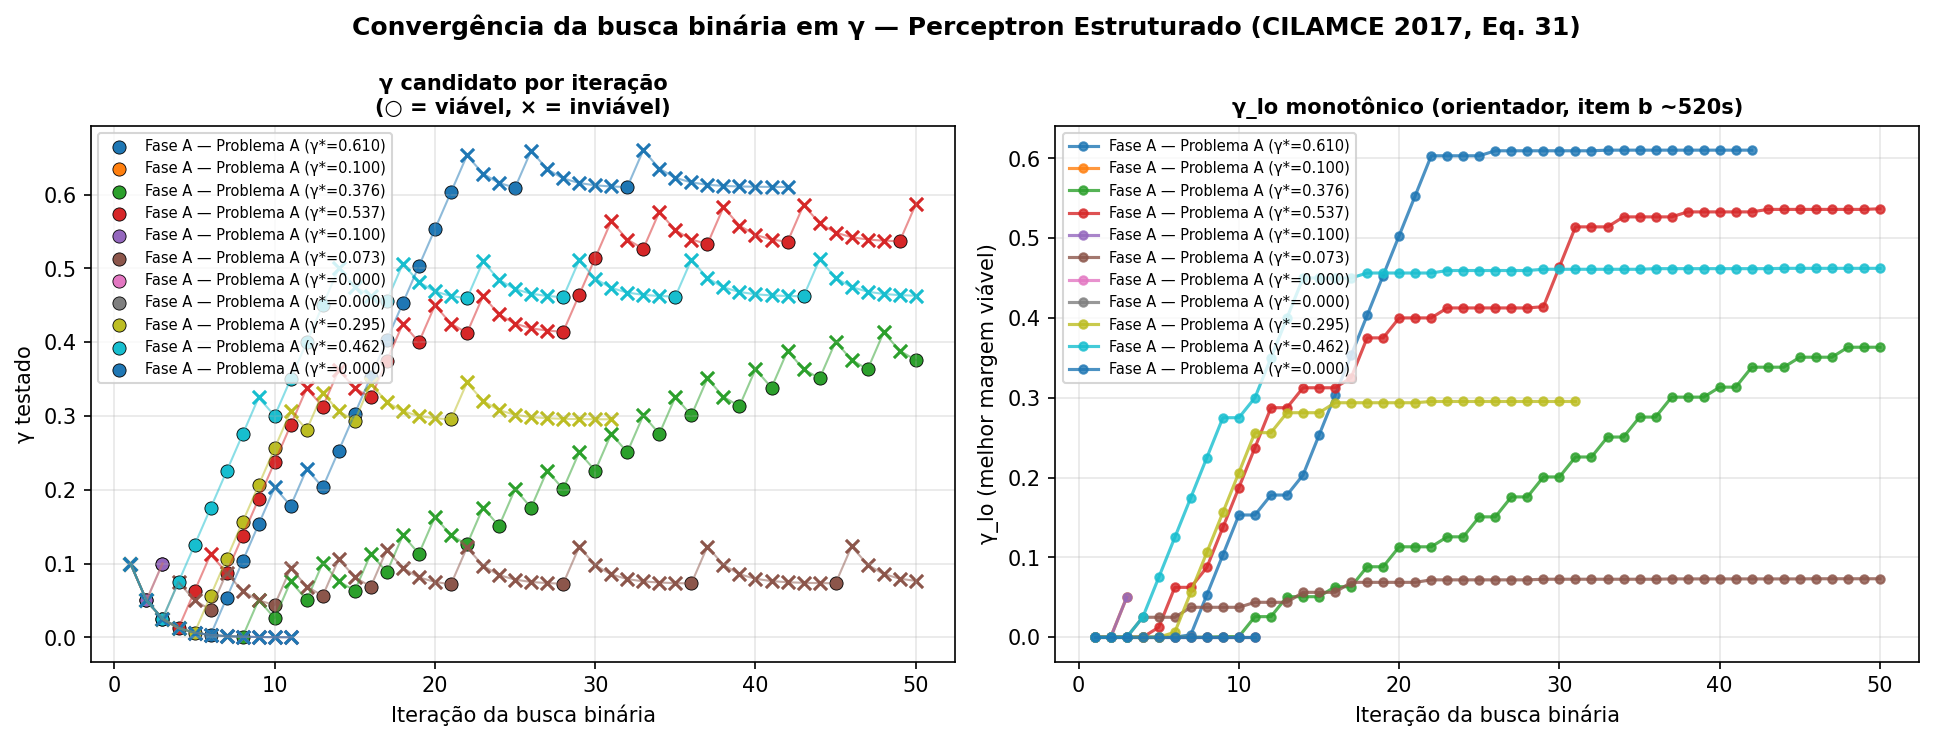
\includegraphics[width=0.85\linewidth,height=0.55\textheight,keepaspectratio]{final_10_gamma_convergence.png}
  \end{center}
  Diagn\'ostico da busca bin\'aria em $\gamma$ (item b reuni\~ao 30/04 $\sim$520s): $\gamma_{\text{lo}}$ monot\^onico crescente verifica converg\^encia.
\end{frame}

% 81
\begin{frame}{D2 --- Limita\c{c}\~oes de reprodutibilidade}
  \footnotesize
  \begin{itemize}
    \item LLM evolui silenciosamente entre execu\c{c}\~oes.
    \item Temperatura $0$ N\~AO garante determinismo (batching GPU).
    \item Usamos 3 seeds $\times$ 3 reps em produ\c{c}\~ao = 9 observa\c{c}\~oes/config.
    \item Estocasticidade residual t\'ipica $< 2\%$ entre reps da mesma seed.
  \end{itemize}
\end{frame}

\end{document}
